% Options for packages loaded elsewhere
\PassOptionsToPackage{unicode}{hyperref}
\PassOptionsToPackage{hyphens}{url}
\PassOptionsToPackage{dvipsnames,svgnames,x11names}{xcolor}
%
\documentclass[
  11pt,
  letterpaper,
]{scrreprt}

\usepackage{amsmath,amssymb}
\usepackage{iftex}
\ifPDFTeX
  \usepackage[T1]{fontenc}
  \usepackage[utf8]{inputenc}
  \usepackage{textcomp} % provide euro and other symbols
\else % if luatex or xetex
  \usepackage{unicode-math}
  \defaultfontfeatures{Scale=MatchLowercase}
  \defaultfontfeatures[\rmfamily]{Ligatures=TeX,Scale=1}
\fi
\usepackage{lmodern}
\ifPDFTeX\else  
    % xetex/luatex font selection
    \setmainfont[]{TeX Gyre Pagella}
\fi
% Use upquote if available, for straight quotes in verbatim environments
\IfFileExists{upquote.sty}{\usepackage{upquote}}{}
\IfFileExists{microtype.sty}{% use microtype if available
  \usepackage[]{microtype}
  \UseMicrotypeSet[protrusion]{basicmath} % disable protrusion for tt fonts
}{}
\makeatletter
\@ifundefined{KOMAClassName}{% if non-KOMA class
  \IfFileExists{parskip.sty}{%
    \usepackage{parskip}
  }{% else
    \setlength{\parindent}{0pt}
    \setlength{\parskip}{6pt plus 2pt minus 1pt}}
}{% if KOMA class
  \KOMAoptions{parskip=half}}
\makeatother
\usepackage{xcolor}
\usepackage{svg}
\setlength{\emergencystretch}{3em} % prevent overfull lines
\setcounter{secnumdepth}{5}
% Make \paragraph and \subparagraph free-standing
\makeatletter
\ifx\paragraph\undefined\else
  \let\oldparagraph\paragraph
  \renewcommand{\paragraph}{
    \@ifstar
      \xxxParagraphStar
      \xxxParagraphNoStar
  }
  \newcommand{\xxxParagraphStar}[1]{\oldparagraph*{#1}\mbox{}}
  \newcommand{\xxxParagraphNoStar}[1]{\oldparagraph{#1}\mbox{}}
\fi
\ifx\subparagraph\undefined\else
  \let\oldsubparagraph\subparagraph
  \renewcommand{\subparagraph}{
    \@ifstar
      \xxxSubParagraphStar
      \xxxSubParagraphNoStar
  }
  \newcommand{\xxxSubParagraphStar}[1]{\oldsubparagraph*{#1}\mbox{}}
  \newcommand{\xxxSubParagraphNoStar}[1]{\oldsubparagraph{#1}\mbox{}}
\fi
\makeatother


\providecommand{\tightlist}{%
  \setlength{\itemsep}{0pt}\setlength{\parskip}{0pt}}\usepackage{longtable,booktabs,array}
\usepackage{calc} % for calculating minipage widths
% Correct order of tables after \paragraph or \subparagraph
\usepackage{etoolbox}
\makeatletter
\patchcmd\longtable{\par}{\if@noskipsec\mbox{}\fi\par}{}{}
\makeatother
% Allow footnotes in longtable head/foot
\IfFileExists{footnotehyper.sty}{\usepackage{footnotehyper}}{\usepackage{footnote}}
\makesavenoteenv{longtable}
\usepackage{graphicx}
\makeatletter
\newsavebox\pandoc@box
\newcommand*\pandocbounded[1]{% scales image to fit in text height/width
  \sbox\pandoc@box{#1}%
  \Gscale@div\@tempa{\textheight}{\dimexpr\ht\pandoc@box+\dp\pandoc@box\relax}%
  \Gscale@div\@tempb{\linewidth}{\wd\pandoc@box}%
  \ifdim\@tempb\p@<\@tempa\p@\let\@tempa\@tempb\fi% select the smaller of both
  \ifdim\@tempa\p@<\p@\scalebox{\@tempa}{\usebox\pandoc@box}%
  \else\usebox{\pandoc@box}%
  \fi%
}
% Set default figure placement to htbp
\def\fps@figure{htbp}
\makeatother
% definitions for citeproc citations
\NewDocumentCommand\citeproctext{}{}
\NewDocumentCommand\citeproc{mm}{%
  \begingroup\def\citeproctext{#2}\cite{#1}\endgroup}
\makeatletter
 % allow citations to break across lines
 \let\@cite@ofmt\@firstofone
 % avoid brackets around text for \cite:
 \def\@biblabel#1{}
 \def\@cite#1#2{{#1\if@tempswa , #2\fi}}
\makeatother
\newlength{\cslhangindent}
\setlength{\cslhangindent}{1.5em}
\newlength{\csllabelwidth}
\setlength{\csllabelwidth}{3em}
\newenvironment{CSLReferences}[2] % #1 hanging-indent, #2 entry-spacing
 {\begin{list}{}{%
  \setlength{\itemindent}{0pt}
  \setlength{\leftmargin}{0pt}
  \setlength{\parsep}{0pt}
  % turn on hanging indent if param 1 is 1
  \ifodd #1
   \setlength{\leftmargin}{\cslhangindent}
   \setlength{\itemindent}{-1\cslhangindent}
  \fi
  % set entry spacing
  \setlength{\itemsep}{#2\baselineskip}}}
 {\end{list}}
\usepackage{calc}
\newcommand{\CSLBlock}[1]{\hfill\break\parbox[t]{\linewidth}{\strut\ignorespaces#1\strut}}
\newcommand{\CSLLeftMargin}[1]{\parbox[t]{\csllabelwidth}{\strut#1\strut}}
\newcommand{\CSLRightInline}[1]{\parbox[t]{\linewidth - \csllabelwidth}{\strut#1\strut}}
\newcommand{\CSLIndent}[1]{\hspace{\cslhangindent}#1}


% Wird für die Tabelle im Titelblatt der Experten verwendet:
% Array
\usepackage{array}
% Neue Definition für Tabelleneinträge
% linksbündig mit Breitenangabe
\newcolumntype{L}[1]{>{\raggedright\arraybackslash}p{#1}} 
% zentriert mit Breitenangabe
\newcolumntype{C}[1]{>{\centering\arraybackslash}p{#1}} 
% rechtsbündig mit Breitenangabe
\newcolumntype{R}[1]{>{\raggedleft\arraybackslash}p{#1}} 

\usepackage[a4paper, margin=3cm]{geometry}

% Titles take mainfont
\addtokomafont{disposition}{\rmfamily}





\usepackage{fvextra}
\DefineVerbatimEnvironment{Highlighting}{Verbatim}{breaklines,commandchars=\\\{\}}
\makeatletter
\@ifpackageloaded{bookmark}{}{\usepackage{bookmark}}
\makeatother
\makeatletter
\@ifpackageloaded{caption}{}{\usepackage{caption}}
\AtBeginDocument{%
\ifdefined\contentsname
  \renewcommand*\contentsname{Inhaltsverzeichnis}
\else
  \newcommand\contentsname{Inhaltsverzeichnis}
\fi
\ifdefined\listfigurename
  \renewcommand*\listfigurename{Abbildungsverzeichnis}
\else
  \newcommand\listfigurename{Abbildungsverzeichnis}
\fi
\ifdefined\listtablename
  \renewcommand*\listtablename{Tabellenverzeichnis}
\else
  \newcommand\listtablename{Tabellenverzeichnis}
\fi
\ifdefined\figurename
  \renewcommand*\figurename{Abbildung}
\else
  \newcommand\figurename{Abbildung}
\fi
\ifdefined\tablename
  \renewcommand*\tablename{Tabelle}
\else
  \newcommand\tablename{Tabelle}
\fi
}
\@ifpackageloaded{float}{}{\usepackage{float}}
\floatstyle{ruled}
\@ifundefined{c@chapter}{\newfloat{codelisting}{h}{lop}}{\newfloat{codelisting}{h}{lop}[chapter]}
\floatname{codelisting}{Listing}
\newcommand*\listoflistings{\listof{codelisting}{Listingverzeichnis}}
\makeatother
\makeatletter
\makeatother
\makeatletter
\@ifpackageloaded{caption}{}{\usepackage{caption}}
\@ifpackageloaded{subcaption}{}{\usepackage{subcaption}}
\makeatother
\makeatletter
\@ifpackageloaded{tcolorbox}{}{\usepackage[skins,breakable]{tcolorbox}}
\makeatother
\makeatletter
\@ifundefined{shadecolor}{\definecolor{shadecolor}{rgb}{.97, .97, .97}}{}
\makeatother
\makeatletter
\@ifundefined{codebgcolor}{\definecolor{codebgcolor}{HTML}{F5F5F5}}{}
\makeatother
\makeatletter
\ifdefined\Shaded\renewenvironment{Shaded}{\begin{tcolorbox}[enhanced, boxrule=0pt, frame hidden, breakable, colback={codebgcolor}, sharp corners]}{\end{tcolorbox}}\fi
\makeatother

\ifLuaTeX
\usepackage[bidi=basic]{babel}
\else
\usepackage[bidi=default]{babel}
\fi
\babelprovide[main,import]{ngerman}
\ifPDFTeX
\else
\babelfont{rm}[]{TeX Gyre Pagella}
\fi
% get rid of language-specific shorthands (see #6817):
\let\LanguageShortHands\languageshorthands
\def\languageshorthands#1{}
\ifLuaTeX
  \usepackage[german]{selnolig} % disable illegal ligatures
\fi
\usepackage{bookmark}

\IfFileExists{xurl.sty}{\usepackage{xurl}}{} % add URL line breaks if available
\urlstyle{same} % disable monospaced font for URLs
\hypersetup{
  pdftitle={Tragverhalten von Stahlbetontragwerken},
  pdfauthor={Pascal Gitz},
  pdflang={de},
  colorlinks=true,
  linkcolor={Black},
  filecolor={Maroon},
  citecolor={Blue},
  urlcolor={Blue},
  pdfcreator={LaTeX via pandoc}}


% TITELBLATT, VERSIONSTABELLE UND SELBSTSTÄNDIGKEITSERKLÄRUNG
%--------------------------------------------------------------------------------------------------------------------


\titlehead{
\includegraphics[height=0.5cm]{../imgs/logos/logo-mse}\hfill
\includegraphics[height=0.5cm]{../imgs/logos/logo-hslu-en-col} \\ }
\subject{MASTER OF SCIENCE IN ENGINEERING\\Masterthesis}
\title{Tragverhalten von Stahlbetontragwerken}

\subtitle
{Modellvorstellungen zur nichtlinearen Verformungsberechnung}

%\thanks{
%Version 1.0
%\hfill \today
%\hfill Hun}


\date{\large Horw, Freitag, 17. Januar 2025}
\author{Pascal Gitz}

\publishers{
	\begin{table}[H]
		\centering
		\begin{tabular}{L{2cm} L{6cm}}
			Advisor: & Prof. FH, Dr. Daniel Heinzmann \\
			Experte: & Dr. Thomas Jäger \\
		\end{tabular}
	\end{table}
}
\begin{document}
\maketitle


Hiermit erkläre ich, dass ich die vorliegende Arbeit selbstständig angefertigt und keine anderen als die angegebenen Hilfsmittel verwendet habe. Sämtliche verwendeten Textausschnitte, Zitate oder Inhalte anderer Verfasser wurden ausdrücklich als solche gekennzeichnet.\\%
%
\\%
%
Horw, 17. Januar 2025 \hfill Pascal Gitz%

\vfill
%\begin{tabular}[h]{llcr} 
    %*Version 2.0 & - Definitives Exemplar & \today & MK \\ 
    %*Version 1.0 & - Prüfungsexemplar & 22. Januar 2021 & MK \\ 
%\end{tabular}\\

% Version 2.0 - Definitives Exemplar \hfill \today \quad \quad \quad \quad \quad MK\\
Version 1.0 - Prüfungsexemplar \hfill 17. Januar 2015 \quad \quad \quad \quad \quad PG\\
Version 0.9 - Entwurf \hfill 10. Januar 2025 \quad \quad \quad \quad \quad PG\\

\newpage

\chapter*{Kurzfassung}

\RecustomVerbatimEnvironment{verbatim}{Verbatim}{
  showspaces = false,
  showtabs = false,
  breaksymbolleft={},
  breaklines
  % Note: setting commandchars=\\\{\} here will cause an error 
}

\renewcommand*\contentsname{Inhaltsverzeichnis}
{
\hypersetup{linkcolor=}
\setcounter{tocdepth}{1}
\tableofcontents
}
\listoffigures

\bookmarksetup{startatroot}

\chapter{Einleitung}\label{einleitung}

Bereits 1935 wurden in der damaligen SIA-Norm 112 Anforderungen an die
Durchbiegung von Stahlbetonbauteilen definiert. Seitdem hat sich die
Gebrauchstauglichkeit, insbesondere die Verformung von Tragwerken, zu
einer zentralen Grösse im Bemessungsablauf entwickelt. Trotz dieser
essenziellen Rolle werden Verformungen im Stahlbetonbau in der heutigen
Baupraxis jedoch häufig nur durch vereinfachte Abschätzungen bewertet.

Solche vereinfachten Ansätze bergen erhebliche Nachteile. Sie können
dazu führen, dass potenzielle Optimierungen übersehen werden, was sich
direkt auf den Materialverbrauch auswirkt. Ein unnötig erhöhter
Materialverbrauch beeinflusst nicht nur die Wirtschaftlichkeit des
Tragwerks negativ, sondern belastet auch dessen Ökobilanz.

Im Gegensatz dazu hat sich in der Forschung die Nutzung nichtlinearer
Finite-Elemente-Methoden (NLFEM) als präzises und effektives Werkzeug
zur Verformungsberechnung etabliert. Programme wie Ansys, Abaqus oder
Atena bieten hohe Genauigkeit und Flexibilität. Diese Werkzeuge stossen
in der praktischen Anwendung jedoch auf zahlreiche Hindernisse: Die
Lizenzkosten sind hoch, die Bestimmung der Vielzahl an Eingabeparametern
erfordert vertieftes Fachwissen und Aufwand, und die Ergebnisse sind oft
schwer zu interpretieren. Darüber hinaus erlauben die
benutzerfreundlichen Eingabemasken dieser Softwares eine rasche
Modellierung komplexer Probleme ohne Verständnis der Hintergründe. Dies
führt oft zu unzureichend begründeten Aussagen.

Die vorliegende Arbeit hat das Ziel, eine praxisorientierte Methode zur
präzisen Berechnung von Verformungen in Stahlbetontragwerken zu
entwickeln. Der Schwerpunkt liegt auf der Kombination von Genauigkeit
und Anwendbarkeit im Berufsalltag, wobei insbesondere die
Nachvollziehbarkeit und Interpretation der Resultate eine zentrale Rolle
spielen.

Im Fokus der Arbeit steht die Modellbildung für die Anwendung bei
Platten- und Stabtragwerken. Dabei wird ausschliesslich das
Biegetragverhalten betrachtet. Zudem werden sämtliche Berechnungen mit
der FE-Software AxisVM-X7 durchgeführt.

Im ersten Kapitel wird die Modellvorstellung aufgezeigt, welche mit
einer Grosszahl an in der Schweiz verbreiteten Statiksoftwares
angewendet werden kann. Es wird lediglich auf die generellen Aspekte des
Modells eingegangen. Danach wird die Anwendung des Modells an einem
zweidimensionalen Stabsystem illustriert und anschliessend auf einen
dreidimensionalen Trägerrost übertragen. Nach der erfolgreichen
Beschreibung dreidimensionaler Systeme wird das Modell auf ein
theoretisches Plattentragwerk angewendet. Den Höhepunkt der Arbeit
bildet die Anwendung des Modells an einem konkreten Versuchsbeispiel.
Abschliessend wird ein Fazit über die erzielten Ergebnisse gezogen und
ein Ausblick auf mögliche zukünftige Forschungsthemen gegeben.

\bookmarksetup{startatroot}

\chapter{Allgemeine Modellbildung}\label{allgemeine-modellbildung}

Um einen Überblick über die Modellbildung zu erhalten wird mit einem
Gedankenexperiment gestartet. Dazu dient das statische System in der
Abbildung~\ref{fig-allg_stat_system} als Grundlage. Es beschreibt einen
einfachen Balken mit einer konstanten Streckenlast belastet. Der Balken
wird mit starren Stäben modelliert, welche mit Drehfedern gekoppelt
sind. In den Drehfedern ist eine linear-elastische
Momenten-Verdrehungs-Beziehung um die globale Y-Achse hinterlegt.

\begin{figure}[H]

\centering{

\pandocbounded{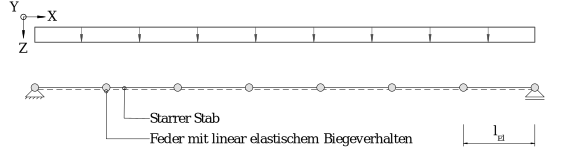
\includegraphics[keepaspectratio]{index_files/mediabag/../imgs/allg_stat_system.pdf}}

}

\caption{\label{fig-allg_stat_system}Beispielsystem eines einfachen
Balkens}

\end{figure}%

Durch die Streckenlast folgt eine Biegeverformung wie in der
Abbildung~\ref{fig-allg_stat_system_def1} gezeigt. Die Stäbe erfahren
eine Starrkörperrotation. Vergleicht man die
Abbildung~\ref{fig-allg_stat_system_def1} mit der
Abbildung~\ref{fig-allg_stat_system_def2}, so ist ersichtlich, dass dies
nicht dem Polygon 4. Grades der analytischen Biegelinie für einen
einfachen Balken entspricht, als numerische Näherung zu dieser jedoch
anwendbar ist.

\begin{figure}[H]

\centering{

\pandocbounded{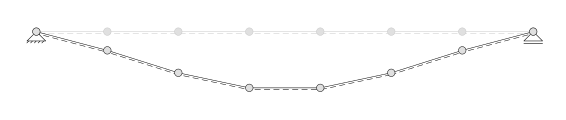
\includegraphics[keepaspectratio]{index_files/mediabag/../imgs/allg_stat_system_def1.pdf}}

}

\caption{\label{fig-allg_stat_system_def1}Bieglinie des einfachen
Balkens mit linear elastischen Federn}

\end{figure}%

Die Modellvorstellung mit linear-elastischen
Momenten-Verdrehungs-Beziehungen weist in erster Linie keinen Mehrwert
zu einer Modellierung mit einem einzelnen Stab auf.

\begin{figure}[H]

\centering{

\pandocbounded{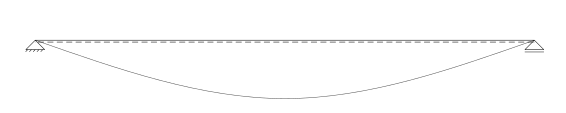
\includegraphics[keepaspectratio]{index_files/mediabag/../imgs/allg_stat_system_def2.pdf}}

}

\caption{\label{fig-allg_stat_system_def2}Analytische Biegelinie des
einfachen Balkens}

\end{figure}%

Der Vorteil dieses Ansatzes liegt darin, dass den Federn anstelle der
elastischen Beziehung, auch nicht-lineare Federbeziehungen hinterlegt
werden können. Dadurch können nicht-lineare Biegelinien numerisch
approximiert werden. Die Erweiterung des Modells ist schematisch in der
Abbildung~\ref{fig-allg_gedankenexp} illustriert.

\begin{figure}[H]

\centering{

\pandocbounded{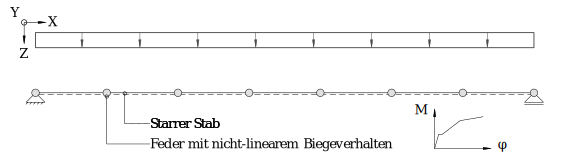
\includegraphics[keepaspectratio]{index_files/mediabag/../imgs/allg_gedankenexp.pdf}}

}

\caption{\label{fig-allg_gedankenexp}Einfacher Balken mit nicht-linearen
Federeigenschaften}

\end{figure}%

Mit dem angepassten System resultiert der qualitative Verlauf der
Biegelinie gemäss der Abbildung~\ref{fig-allg_stat_system_def_nl}. Es
ist ersichtlich, dass sich das System in den Randbereichen steifer
verhält als in der Feldmitte. Beziehungsweise ist das System bei
niedrigeren Biegemomenten steifer.

\begin{figure}[H]

\centering{

\pandocbounded{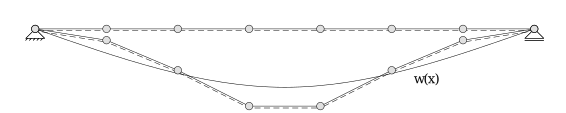
\includegraphics[keepaspectratio]{index_files/mediabag/../imgs/allg_stat_system_def_nl.pdf}}

}

\caption{\label{fig-allg_stat_system_def_nl}Bieglinie des einfachen
Balkens mit nicht-linearen Federn, ergänzt mit elastischer Biegelinie}

\end{figure}%

Das Gedankenexperiment lässt sich mit der Kernaussage abschliessen, dass
das System an sich nicht komplex ist. Die Qualität der gewünschten
Resultate jedoch einzig von der Bestimmung der Federsteifigkeiten
abhängt.

\section{Berechnungsschema}\label{berechnungsschema}

Die Modellbildung kann mit dem Ablaufschema gemäss der
Abbildung~\ref{fig-allg_schema} verallgemeinert werden. Diese ist
grundsätzlich Software unabhängig. Die FE-Software muss lediglich in der
Lage sein, nichtlineare Federsteifigkeiten berechnen zu können.

\begin{figure}[H]

\centering{

\pandocbounded{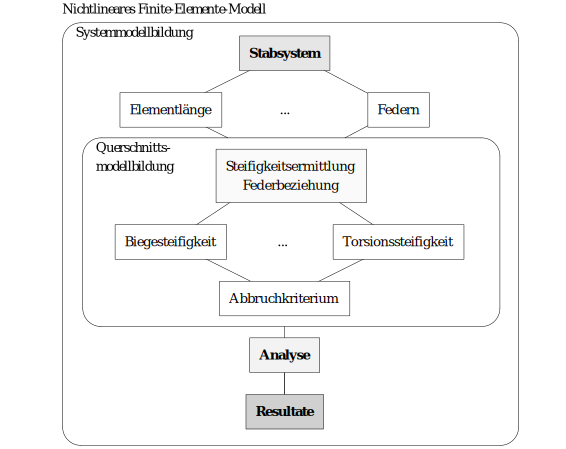
\includegraphics[keepaspectratio]{index_files/mediabag/../imgs/allg_schema.pdf}}

}

\caption{\label{fig-allg_schema}Modellierungsschema}

\end{figure}%

Dabei wird zwischen dem gesamten statischen System, betitelt mit
Systemmodellbildung, und der Steifigkeitsermittlung, sowie der
Definition des Abbruchkriteriums, bezeichnet als
Querschnittsmodellbildung, unterschieden.

\section{Systemmodellbildung}\label{systemmodellbildung}

Die Systemmodellbildung wurde mit dem einleitenden Gedankenexperiment
illustriert. In folgendem Abschnitt wird auf modellspezifische
Einzelheiten eingegangen. Das Ziel ist es das Modellverhalten zu
erläutern. Auf die Abbruchkriterien, Steifigkeitsermittlungen, sprich
Querschnittsmodellbildung wird in den folgenden Anwendungsfällen
eingegangen.

\subsection{Elementlänge}\label{elementluxe4nge}

Die Elementlänge definiert die Länge der starren Stäbe, gemessen von
Feder zu Feder. Dargestellt ist die Elementlänge in der
Abbildung~\ref{fig-allg_stat_system}.

Dabei stellt sich die zentrale Frage, wie gross die Elementlänge zu
wählen ist. Aus der Abbildung~\ref{fig-allg_stat_system_def1} wird
ersichtlich, dass durch eine Minimierung der Elementlänge \(l_{El}\),
sich das Biegeverhalten des Systems der analytischen Lösung annähert.
Somit gilt, die Elementlänge ist so gross wie möglich, so klein wie
nötig zu wählen.

Grundsätzlich ist die Elementlänge anhand einer Sensitivitätsanalyse zu
bestimmen. Dabei sollten Modelle mit der Variation der Elementlänge
berechnet werden und dadurch den Einfluss der Elementlänge bestimmt
werden.

Betrachtet man das Biegetragverhalten, so ist naheliegend, dass bei
grossen Biegemomentengradienten eine kleine Elementlänge zu präziseren
Resultaten führt.

\subsection{Federn}\label{federn}

Die Feder verbindet die starren Stäbe, wie in der
Abbildung~\ref{fig-allg_stat_system} gezeigt. Zunächst wird das
Verhalten der Feder illustriert. Verbleibt man beim Gedankenexperiment
bei den Biegeverformungen, so integriert die Drehfeder die
Biegekrümmungen zu einer Biegeverdrehung. Die Grenzen der Integration
werden über eine Einzugslänge definiert. Die Einzugslänge ist dabei
definiert durch die Hälfte der Distanz bis zum nächsten Gelenk.

\begin{figure}[H]

\centering{

\pandocbounded{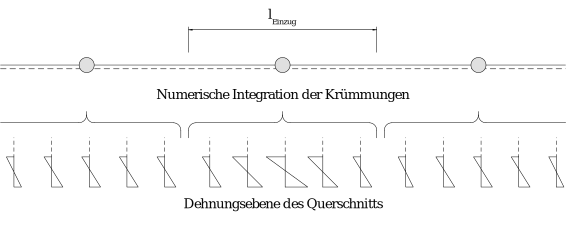
\includegraphics[keepaspectratio]{index_files/mediabag/../imgs/allg_feder.pdf}}

}

\caption{\label{fig-allg_feder}Numerische Integration der Krümmungen
mittels den Feder}

\end{figure}%

Generell lassen sich den Federn entsprechend den Freiheitsgraden
Beziehungen hinterlegen. Im zweidimensionalen Raum entspricht dies drei
Beziehungen, im dreidimensionalen Raum erweitert sich dies zu deren
sechs.

Gelenkdefinitionen im zweidimensionalen Raum:

\begin{equation}\phantomsection\label{eq-zweidim_gelenkfunktionen}{
F_x(u_z),F_z(u_z),M_y(\varphi_y)
}\end{equation}

Gelenkdefinitionen im dreidimensionalen Raum:

\begin{equation}\phantomsection\label{eq-dreidim_gelenkfunktionen}{
F_x(u_x),F_y(u_y),F_z(u_z),M_x(\varphi_x),M_y(\varphi_y),M_z(\varphi_z)
}\end{equation}

Dabei steht \(u_i\) für die Verformung, \(F_i\) für die Kraft, \(M_i\)
für das Biegemoment und \(\varphi_i\) für die Verdrehung und der Index
\(i\) für die entsprechende Richtung. Dies verdeutlicht, dass mit der
richtigen Wahl der Federbeziehungen das nicht-lineare Querkraft-,
Normalkraft- und Biegeverhalten modelliert werden kann. Die
Schwierigkeit liegt jedoch offensichtlich in der richtigen Wahl der
Federbeziehungen.

Modelliert wird in AxisVM-X7 nicht mit einer Feder, sondern mit einem
Stabgelenk. Das Stabgelenk ist im Gegensatz zur Feder unendlich klein,
was die Präzision des Systems verbessert. Zudem reduziert sich der
Modellierungsaufwand. Die Federn werden fortan als Stabgelenke
bezeichnet.

Des Weiteren wird eine Modellierungsstrategie gewählt bei der an jedem
Stab ein Anfang- und ein Endgelenk modelliert wird. Dies bringt den
Vorteil, dass die Einzugslängen sich für Randgelenke, bei Auflagern
beispielsweise, nicht unterscheiden. Illustriert ist dies in der
Abbildung~\ref{fig-allg_doppelgelenk}.

\begin{figure}[H]

\centering{

\pandocbounded{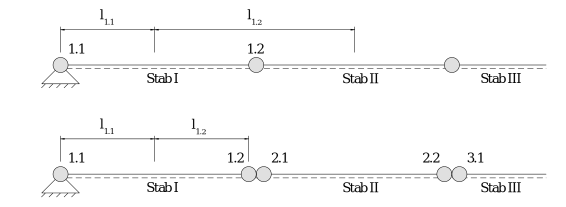
\includegraphics[keepaspectratio]{index_files/mediabag/../imgs/allg_doppelgelenk.pdf}}

}

\caption{\label{fig-allg_doppelgelenk}Modellierungsstrategie der
Stabanfang- und Endgelenke}

\end{figure}%

\subsection{Analyse}\label{analyse}

Auf einen vertieften Beschrieb des Lösungsalgorithmus des nicht-linearen
Systems wird verzichtet. In AxisVM-X7 ist der Newton-Rhapson-Algorithmus
implementiert zur iterativen Lösung des Systems.

Als Nutzer ist die Tatsache wertvoll, dass eine nicht-lineare Berechnung
in Lastinkrementen funktioniert. Es wird ein definierter Anteil der Last
auf das System gebracht, die Steifigkeit der Gelenke aus den
Zustandslinien der Schnittgrössen ermittelt und versucht die Differenz
zwischen den inneren Kräften und den Einwirkungen zu minimieren.

\subsection{Resultate}\label{resultate}

Nach der nicht-linearen Analyse lassen sich eine Vielzahl von Resultaten
ausgeben. Die starren Stäbe weisen die üblichen Schnittkräfte auf.
Lagerreaktion lassen sich darstellen. Zudem besteht die Möglichkeit zur
Darstellung der relativen Gelenkrotation der Stabgelenke. Die Definition
der relativen Gelenkrotation \(\theta_R\) ist in der
Abbildung~\ref{fig-allg_relative_gelenkrot} aufgezeigt.

\begin{figure}[H]

\centering{

\pandocbounded{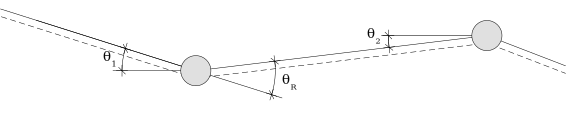
\includegraphics[keepaspectratio]{index_files/mediabag/../imgs/allg_relative_gelenkrot.pdf}}

}

\caption{\label{fig-allg_relative_gelenkrot}Relative Gelenkrotation am
verformten System}

\end{figure}%

Diese ist von besonderem Interesse, da daraus die Steifigkeit des
Gelenks abgelesen werden kann. Somit kann für jedes Gelenk die Position
in der Momenten-Verdrehungs-Beziehung ermittelt werden und eine Aussage
auf den Zustand gegeben werden.

\section{Querschnittsmodellbildung}\label{querschnittsmodellbildung}

\subsection{Stabquerschnitt}\label{stabquerschnitt}

Die Querschnittsmodellbildung ist für einen Stabquerschnitt und ein
Plattenquerschnitt gesondert zu betrachten.

\subsubsection{Biegesteifigkeit}\label{biegesteifigkeit}

Generell kann die Biegesteifigkeit anhand einer
Momenten-Krümmungs-Beziehung beschrieben werden. Dazu sind für den
Betonstahl und den Beton Spannungs-Dehnungs-Beziehungen zu modellieren.
Anhand dieser kann der Querschnitt bei steigender Krümmung, dargestellt
in der Abbildung~\ref{fig-allg_qs_analyse}, untersucht werden.

\begin{figure}[H]

\centering{

\pandocbounded{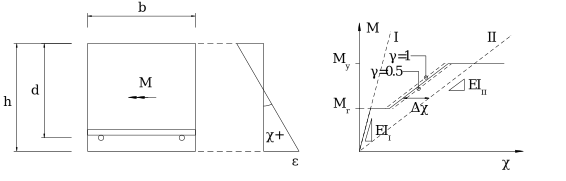
\includegraphics[keepaspectratio]{index_files/mediabag/../imgs/allg_qs_analyse.pdf}}

}

\caption{\label{fig-allg_qs_analyse}Querschnittsanalyse des
Beispielquerschnitts, Dehnungsebenen}

\end{figure}%

Die Gleichung~\ref{eq-zweidim_gelenkfunktionen} verdeutlicht, dass eine
Momenten-Verdrehungs-Beziehung gefordert ist. Wie die
Abbildung~\ref{fig-allg_feder} zeigt, entspricht die Verdrehung der
Integration der Krümmung über die Einzugslänge. Folglich lässt sich die
Momenten-Verdrehungs-Beziehung durch Multiplikation der Krümmung mit der
Einzugslänge ermitteln.

\begin{equation}\phantomsection\label{eq-chi_to_phi_y}{
M_y(\varphi_y) = M_y(\chi_y \cdot l_{Einzug})
}\end{equation}

Hält man sich an die Modellierungsstrategie, gemäss der
Abbildung~\ref{fig-allg_doppelgelenk}, so ist die Einzugslänge durch die
Gleichung~\ref{eq-einzug_doppelgelenk} definiert.

\begin{equation}\phantomsection\label{eq-einzug_doppelgelenk}{
l_{Einzug} = \frac{l_{El}}{2}
}\end{equation}

Es ist selbstverständlich, dass die Momenten-Verdrehungs-Beziehung nur
für den analysierten Querschnitt gilt. Bei einer Querschnittsänderung
ist eine angepasste Momenten-Verdrehungs-Beziehung zu bestimmen.

\subsection{Plattenquerschnitt}\label{plattenquerschnitt}

Die Querschnittsmodellbildung lässt sich allgemein an einem
Plattenausschnitt beschreiben. Dazu ist der Querschnitt gemäss der
Abbildung~\ref{fig-allg_qs_mikro} gewählt. Der Streifen der
Stahlbetonplatte weist eine Streifenbreite \(b_w\) und eine Höhe \(h\)
auf.

\begin{figure}[H]

\centering{

\pandocbounded{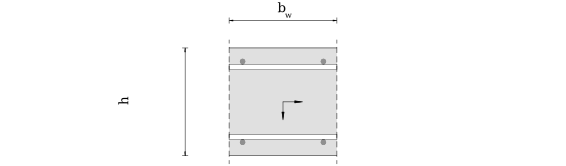
\includegraphics[keepaspectratio]{index_files/mediabag/../imgs/allg_qs_mikro.pdf}}

}

\caption{\label{fig-allg_qs_mikro}Beispielquerschnitt der allgemeinen
Querschnittsmodellbildung}

\end{figure}%

Grundüberlegung der Transformation eines Plattenelements auf ein
Balkenelement. In der Abbildung~\ref{fig-allg_platte_zu_balken_sg} ist
ein Plattenelement und ein Balkenelement zu sehen. Das Ziel ist es die
Steifigkeit am Plattenelement in der X-Richtung zu bestimmen und auf ein
Balkenelement zu übertragen. Die Schnittflächen sind dabei grau
hinterlegt.

\begin{figure}[H]

\centering{

\pandocbounded{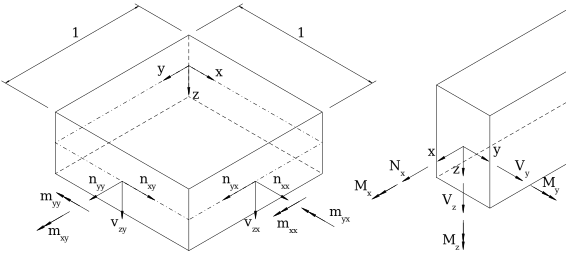
\includegraphics[keepaspectratio]{index_files/mediabag/../imgs/allg_platte_zu_balken_sg.pdf}}

}

\caption{\label{fig-allg_platte_zu_balken_sg}Schnittgrössen am
Plattenelement links, Schnittgrössen am Balkenelement rechts}

\end{figure}%

Dabei sind die Spannungen beim Plattenelement gemäss der
Abbildung~\ref{fig-allg_platte_spannungen} definiert.

\begin{figure}[H]

\centering{

\pandocbounded{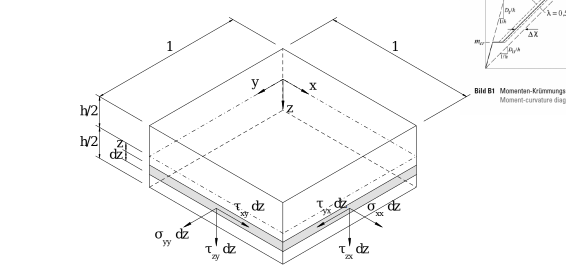
\includegraphics[keepaspectratio]{index_files/mediabag/../imgs/allg_platte_spannungen.pdf}}

}

\caption{\label{fig-allg_platte_spannungen}Spannungen am Plattenelement}

\end{figure}%

Die kinematischen Grössen des Plattenelements zeigt die
Abbildung~\ref{fig-allg_platte_kin}.

\begin{figure}[H]

\centering{

\pandocbounded{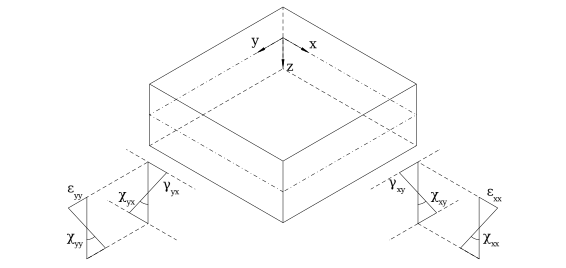
\includegraphics[keepaspectratio]{index_files/mediabag/../imgs/allg_platte_kin.pdf}}

}

\caption{\label{fig-allg_platte_kin}Kinematische Grössen am
Plattenelement}

\end{figure}%

Die Normalspannungen des Balkenelements sind in der
Abbildung~\ref{fig-allg_balken_normal} gezeigt.

\begin{figure}[H]

\centering{

\pandocbounded{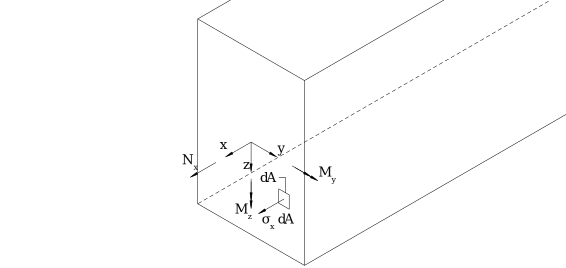
\includegraphics[keepaspectratio]{index_files/mediabag/../imgs/allg_balken_normal.pdf}}

}

\caption{\label{fig-allg_balken_normal}Normalspannungen am Balken}

\end{figure}%

Die Schubspannungen des Balkenelements sind in der
Abbildung~\ref{fig-allg_balken_normal} gezeigt.

\begin{figure}[H]

\centering{

\pandocbounded{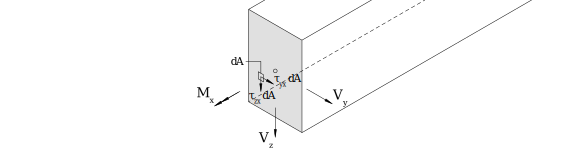
\includegraphics[keepaspectratio]{index_files/mediabag/../imgs/allg_balken_schub.pdf}}

}

\caption{\label{fig-allg_balken_schub}Schubspannungen am Balken}

\end{figure}%

Die kinematischen Grössen des Plattenelements zeigt die
Abbildung~\ref{fig-allg_balken_kin}.

\begin{figure}[H]

\centering{

\pandocbounded{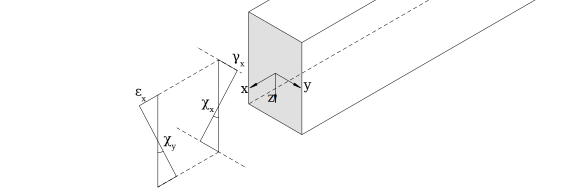
\includegraphics[keepaspectratio]{index_files/mediabag/../imgs/allg_balken_kin.pdf}}

}

\caption{\label{fig-allg_balken_kin}Kinematische Grössen am Balken}

\end{figure}%

\subsubsection{Biegesteifigkeit}\label{biegesteifigkeit-1}

Betrachtet man die Spannungen am Plattenelement, übt Gleichgewicht an
diesem, so folgt die für das Biegemoment an der grau hinterlegten
Fläche, die Beziehung gemäss der Gleichung~\ref{eq-sg_platte_normal}.
\begin{equation}\phantomsection\label{eq-sg_platte_normal}{
\begin{aligned}
&m_{xx} = \int_{-h/2}^{h/2} z \cdot \sigma_{xx}  dz \quad
% &m_{yy} = \int_{-h/2}^{h/2} \sigma_{yy} \cdot z dz \quad
% &m_{xy} = \int_{-h/2}^{h/2} \tau_{xy} \cdot z dz \quad
\end{aligned}
}\end{equation}

\begin{equation}\phantomsection\label{eq-sg_normal_balken}{
\begin{aligned}
% &N_x = \int_A \sigma_x dA \quad
&M_y = \int_A z \cdot \sigma_x dA \quad
% &M_z = \int_A y \cdot \sigma_x dA
\end{aligned}
}\end{equation}

Vergleicht aus der Gleichung~\ref{eq-sg_platte_normal} und
Gleichung~\ref{eq-sg_normal_balken} die Biegemomente \(m_{xx}\) und
\(M_y\) so ist deren Definition analog. Daraus folgt, dass die
Biegesteifigkeit von Plattenelementen direkt übertragbar ist. Es folgt
die Transformationsbeziehung gemäss der
Gleichung~\ref{eq-transformation_biegung}. Diese ist analog der
Gleichung~\ref{eq-chi_to_phi_y} für einen Querschnitt der Breite \(b_w\)

\begin{equation}\phantomsection\label{eq-transformation_biegung}{
M_y(\varphi_y) = b_w \cdot m_{xy}(\chi_{xy}\cdot l_{Einzug})
}\end{equation}

\subsubsection{Torsionssteifigkeit}\label{torsionssteifigkeit}

\begin{equation}\phantomsection\label{eq-sg_platte_drill}{
\begin{aligned}
&m_{xy} = \int_{-h/2}^{h/2} z \cdot \tau_{xy}  dz \quad
\end{aligned}
}\end{equation}

\begin{equation}\phantomsection\label{eq-sg_schub_balken}{
\begin{aligned}
% &V_y = \int_A \tau_yx dA \quad
% &V_z = \int_A \tau_zx dA \quad
&M_x = T = \int_A \left(z \cdot \tau_{yx} - y \cdot \tau_{zx}\right) dA
\end{aligned}
}\end{equation}

Dabei stellt man fest, dass das Torsionsmoment \(M_x\) und das
Drillmoment \(m_{xy}\) unterschiedlich definiert sind. Es fehlen die
vertikal gerichteten Schubspannungen im Plattenelement.

Der Einfluss dieser Tatsache lässt sich an einem einfachen Beispiel
illustrieren. Betrachtet man einen unendlich schmalen Streifen
\(t << b\), dargestellt in der
Abbildung~\ref{fig-allg_torsion_balken_vs_platte}.

\begin{figure}[H]

\centering{

\pandocbounded{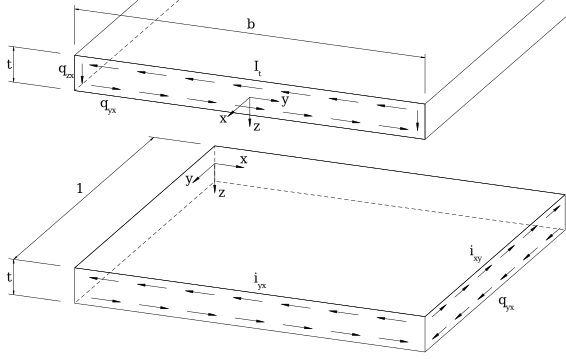
\includegraphics[keepaspectratio]{index_files/mediabag/../imgs/allg_torsion_balken_vs_platte.pdf}}

}

\caption{\label{fig-allg_torsion_balken_vs_platte}Torsionsträgheitsmoment
für einen unendlich schmalen Streifen, darunter für ein unendlich
schmales Plattenelement, nachgezeichnet nach
{[}\citeproc{ref-blaauwendraad_plates_2010}{1}{]}}

\end{figure}%

\begin{equation}\phantomsection\label{eq-torsion_streifen}{
\begin{aligned}
I_t = \frac{bt^3}{3} \quad 
i_{xy} = \frac{t^3}{6}
\end{aligned}
}\end{equation}

Das Torsionsträgheitsmoment des Balkenelements \(I_t\) und das auf die
Einheitslänge bezogene Torsionsträgheitsmoment des Plattenelements in
X-Richtung \(i_{xy}\) unterscheiden sich um den Faktor 2. Der Faktor 2
ist zudem konstant. Dies lässt sich erklären, dass sich beim
Balkenquerschnitt der Schubfluss in Y Richtung zu gleichen Teilen am
Torsionsmoment beteiligt, wie der in X gerichtete Schubfluss. Der
vertikale Schubfluss verläuft zwar nur über die Querschnittshöhe \(t\),
besitzt jedoch den deutlich grösseren Hebelarm, während der horizontale
Schubfluss über die gesamte Breite \(b\) verläuft, mit einem jedoch
deutlich kleineren Hebelarm. Die Gleichung~\ref{eq-schubfluss_balken}
beschreibt diese Tatsache.

\begin{equation}\phantomsection\label{eq-schubfluss_balken}{
M_{x,vert} = q_{zx} \cdot t \cdot b/2 = M_{x,horiz} = q_{yx} \cdot b \cdot t/2 = M_x / 2
}\end{equation}

Die Quintessenz ist somit, dass eine am Plattenelement hergeleitete
Drillsteifigkeit mit dem Faktor 2 zu multiplizieren ist um die
gleichwertige Torsionssteifigkeit am Balken zu erhalten. Beschrieben ist
diese Tatsache ebenfalls in
{[}\citeproc{ref-blaauwendraad_plates_2010}{1}{]} Seite 389.

Transformieren lässt sich die Momenten-Krümmungs-Beziehung des
Plattenelements in die des Balkenelements mit der
Gleichung~\ref{eq-transformation_drill}.

\begin{equation}\phantomsection\label{eq-transformation_drill}{
M_x(\varphi_x) = b_w \cdot m_{xy}(\chi_{xy}\cdot l_{Einzug}) \cdot 2
}\end{equation}

\paragraph{Ungerissene
Drillsteifigkeit}\label{ungerissene-drillsteifigkeit}

Mit dem vorangegangen Beschrieb ist die Transformation der
Drillsteifigkeit auf die Torsionssteifigkeit geklärt. Nun gilt es die
Drillsteifigkeit am Plattenelement zu bestimmen.

Betrachtet man die kinematischen Grössen in
Abbildung~\ref{fig-allg_platte_kin}, so lässt sich die Beziehung
zwischen Biegemoment und Krümmung aufstellen. Dies ist für ein
homogenes, isotropes Plattenelement in der
Gleichung~\ref{eq-ung_drillsteifigkeit} gezeigt.

\begin{equation}\phantomsection\label{eq-drillmoment_von_kruemmung}{
m_{xy} = G i_{xy} \cdot \chi_{xy}
}\end{equation}

\begin{equation}\phantomsection\label{eq-schubmodul}{
G = \frac{E}{2(1-\nu)}
}\end{equation}

\begin{equation}\phantomsection\label{eq-traegheitsmoment_platte}{
i_{xy} = \frac{h^3}{6}
}\end{equation}

\begin{equation}\phantomsection\label{eq-ung_drillsteifigkeit}{
G i_{xy} = \frac{h^3 E}{12(1-\nu)}
}\end{equation}

Das Rissmoment lässt sich bestimmen durch die Substitution der
Schubspannung mit der Betonzugfestigkeit. Dazu folgt das Rissmoment
entsprechend einer Biegeanalyse

\begin{equation}\phantomsection\label{eq-rissdrillmoment}{
m_{xy,r} = f_{ct} \cdot \frac{h^2}{6}
}\end{equation}

\paragraph{Gerissene Drillsteifigkeit}\label{gerissene-drillsteifigkeit}

Die gerissene Drillsteifigkeit wird mittels dem klassischen
Sandwichmodell bestimmt. Das klassische Sandwichmodell ist in
{[}\citeproc{ref-heinzmann_stringer-tafelmodelle_2012}{2}{]}
beschrieben. Mittels diesem ist das Plattenelement in ein Kern und zwei
Deckel zu unterteilen. Den Deckeln sind die Biege- und Drillmomente
zugeordnet, dem Kern die Querkraft.

\begin{figure}[H]

\centering{

\pandocbounded{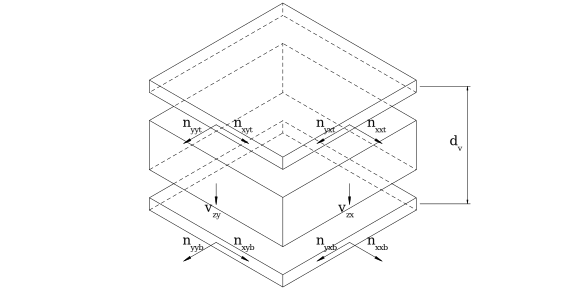
\includegraphics[keepaspectratio]{index_files/mediabag/../imgs/allg_sandwich.pdf}}

}

\caption{\label{fig-allg_sandwich}klassiches Sandwichmodell}

\end{figure}%

Dabei sind die Biegemomente als Kräftepaar auf die Deckel aufgeteilt.

Betrachtet man die Drillmomente gesondert, so stellt sich ein Schubfluss
entlang der Deckel ein. Die Deckel sind als Scheiben unter reiner
Schubbeanspruchung zu betrachten.

\begin{figure}[H]

\centering{

\pandocbounded{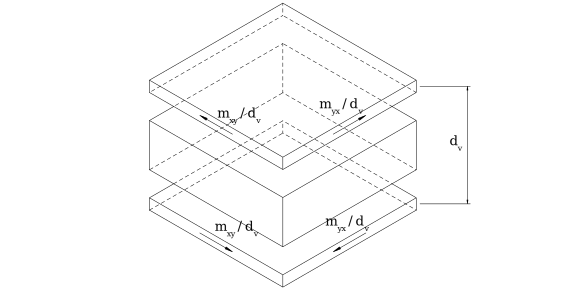
\includegraphics[keepaspectratio]{index_files/mediabag/../imgs/allg_drill_deckel.pdf}}

}

\caption{\label{fig-allg_drill_deckel}Aufteilung der Drillmomente auf
die Deckel gemäss dem klassischen Sandwichmodell}

\end{figure}%

\begin{figure}[H]

\centering{

\pandocbounded{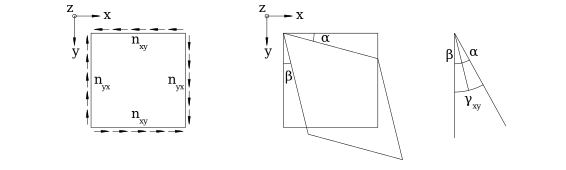
\includegraphics[keepaspectratio]{index_files/mediabag/../imgs/allg_scheibe_schubfluss.pdf}}

}

\caption{\label{fig-allg_scheibe_schubfluss}Scheibe unter reinem Schub,
rechts im Verzerrungszustand}

\end{figure}%

\begin{equation}\phantomsection\label{eq-schubfluss_scheibe}{
n_{xy} = \frac{m_{xy}}{d_v} = n_{yx} = \frac{m_{yx}}{d_v}
}\end{equation}

\begin{equation}\phantomsection\label{eq-schubspannung_scheibe}{
\tau_{xy} = \frac{n_{xy}}{t}
}\end{equation}

\(t\) Deckelstärke

\begin{figure}[H]

\centering{

\pandocbounded{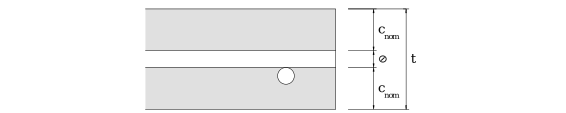
\includegraphics[keepaspectratio]{index_files/mediabag/../imgs/allg_sandwich_deckelstaerke.pdf}}

}

\caption{\label{fig-allg_sandwich_deckelstaerke}Definition der
Deckelstärke}

\end{figure}%

Die Schiebung einer gerissenen Scheibe lässt sich anhand des klassischen
Druckfeldmodells bestimmen. Dieses ist ebenfalls in
{[}\citeproc{ref-heinzmann_stringer-tafelmodelle_2012}{2}{]}
beschrieben.

\begin{equation}\phantomsection\label{eq-schiebung_klass_druckfeldmodell}{
\gamma_{xy} = 2 \frac{\tau_{xy}}{E_s}\cdot \left(\sqrt{\frac{(1+n\rho_x)(1+n\rho_y)}{\rho_x \rho_y}+n} \right)
}\end{equation}

Mit der Gleichung~\ref{eq-schiebung_klass_druckfeldmodell} lässt sich
die Schiebung einer gerissenen Scheibe beschreiben. Diese ist Abhängig
von der Bewehrung des Deckels und kann für den oberen und unteren Deckel
gesondert betrachtet werden.

\begin{figure}[H]

\centering{

\pandocbounded{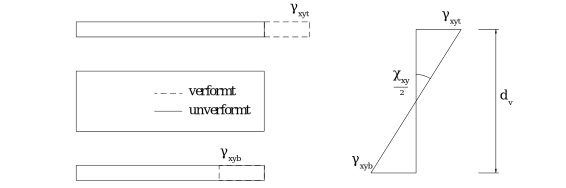
\includegraphics[keepaspectratio]{index_files/mediabag/../imgs/allg_sandwich_kruemmung.pdf}}

}

\caption{\label{fig-allg_sandwich_kruemmung}Ansicht des Sandwichmodells,
resultierende Dehnungsebene durch die Schiebung des oberen und unteren
Deckels}

\end{figure}%

\begin{equation}\phantomsection\label{eq-kruemmung_sandwich}{
\chi_{xy} = \frac{\gamma_{xyt}+ \gamma_{xyb}}{d_v}
}\end{equation}

Abschliessend kann die Momenten-Verdrehungs-Beziehung mit der
Gleichung~\ref{eq-transformation_drill} bestimmt werden.

\bookmarksetup{startatroot}

\chapter{Anwendung Zweifeldträger}\label{sec-zweifeldtraeger}

Im vorangegangen Kapitel wurde vertieft auf die Systemmodellbildung
eingegangen. Sowie wurde diese allgemein formuliert. Dabei wurde die
Querschnittsmodellbildung aussenvor gelassen.

Das Ziel dieses Kapitel ist es an einem konkreten Beispiel die
Systemmodellbildung aufzuzeigen, sowie speziell auf die
Querschnittsmodellbildung einzugehen.

Das Beispiel dazu wurde aus den Vorlesungsunterlagen
{[}\citeproc{ref-jager_stahlbeton_2009}{3}{]} entnommen. Für die
detaillierte analytische Berechnungen ist der
Anhang~\ref{sec-zweifeldtraeger_anhang} zu konsultieren. Sowie ist die
numerische Näherung mit der beschriebenen Modellbildung aufgezeigt. Hier
werden die wichtigsten Erkenntnisse zusammengefasst beschrieben.

\section{Aufgabenbeschrieb}\label{aufgabenbeschrieb}

Zunächst wird auf die Grundlagen des Beispiels eingegangen. Die
Abbildung~\ref{fig-jag_system} zeigt ein statisches System eines
Zweifeldträgers mit den entsprechenden Abmessungen. Der Zweifeldträger
wird mit einer konstanten Streckenlast \(q\) belastet.

\begin{figure}[H]

\centering{

\pandocbounded{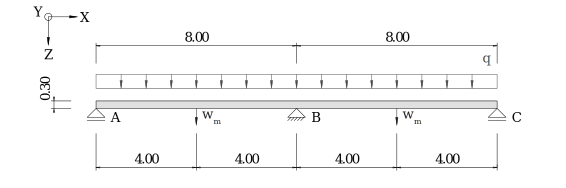
\includegraphics[keepaspectratio]{index_files/mediabag/../imgs/jag_system.pdf}}

}

\caption{\label{fig-jag_system}Statisches system des Zweifeldträgers}

\end{figure}%

Der dazugehörige Querschnitt ist in der
Abbildung~\ref{fig-jag_system_qs} dargestellt. Dargestellt ist die
Biegebewehrung mit entsprechendem Durchmesser.

\begin{figure}[H]

\centering{

\pandocbounded{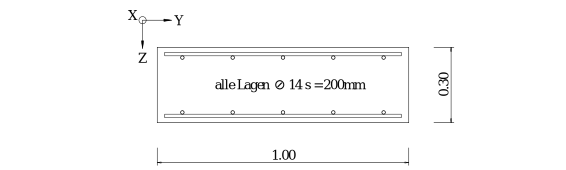
\includegraphics[keepaspectratio]{index_files/mediabag/../imgs/jag_system_qs.pdf}}

}

\caption{\label{fig-jag_system_qs}Querschnitt des Zweifeldträgers}

\end{figure}%

Das übergeordnete Ziel ist es das Last-Verformungs-Verhalten (An der
Stelle des Verformungsvektors \(w_m\), gemäss der
Abbildung~\ref{fig-jag_system}) des Tragwerks für zwei unterschiedlich
duktile Betonstähle zu berechnen. Sprich damit den Einfluss der
Duktilität auf das Tragverhalten zu zeigen.

\subsection{Materialeigenschaften}\label{materialeigenschaften}

Die Betonstähle werden durch die Spannungs-Dehnungs-Diagramme, gemäss
der Abbildung~\ref{fig-jag_stress_strain_b500a} definiert. Es wird ein
bilinearer Verlauf für den B500A und ein trilinearer Verlauf für den
B500C angesetzt.

\begin{figure}[H]

\centering{

\pandocbounded{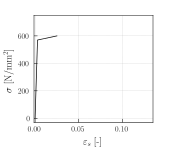
\includegraphics[keepaspectratio]{index_files/mediabag/../imgs/jag_stress_strain_b500a.pdf}}

}

\caption{\label{fig-jag_stress_strain_b500a}Spannungs-Dehnungs-Beziehungen
des Betonstahls B500A}

\end{figure}%

\begin{figure}[H]

\centering{

\pandocbounded{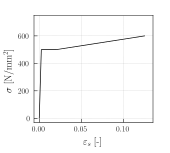
\includegraphics[keepaspectratio]{index_files/mediabag/../imgs/jag_stress_strain_b500c.pdf}}

}

\caption{\label{fig-jag_stress_strain_b500c}Spannungs-Dehnungs-Beziehungen
des Betonstahls B500C}

\end{figure}%

Spannungs-Dehnungs-Diagramme der beiden Betonstähle

\section{Analytische Lösung}\label{analytische-luxf6sung}

Die analytische Lösung erweist sich als umfangreich. Deshalb ist die
detaillierte Berechnung in den Anhang~\ref{sec-zweifeldtraeger_anhang}
verschoben. Das Vorgehen wird dennoch beschrieben.

Betrachtet man das System, dargestellt in der
Abbildung~\ref{fig-jag_system}, unter steigender Belastung, so ist
naheliegend, dass sich über dem Mittelauflager zuerst ein plastisches
Gelenk bildet. Falls genügend Rotationsvermögen vorhanden ist, bildet
sich in Feldmitte ebenfalls ein plastisches Gelenk. Aufgezeigt ist der
Mechanismus in der Abbildung~\ref{fig-jag_mechanismus}.

\begin{figure}[H]

\centering{

\pandocbounded{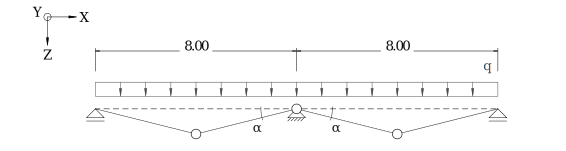
\includegraphics[keepaspectratio]{index_files/mediabag/../imgs/jag_mechanismus.pdf}}

}

\caption{\label{fig-jag_mechanismus}Mechanismus des Zweifeldträgers mit
eingezeichnetem Verdrehungswinkel}

\end{figure}%

Eine zentrale Grösse ist folglich das Rotationsvermögen der plastischen
Gelenke. Um dieses abzuschätzen wird ein Zugglied analysiert. Für den
Zustand des Fliessens der Bewehrung und den Zustand beim Erreichen der
Zugfestigkeit wird eine mittlere Dehnung über das Zugglied ermittelt.
Mit der Dehnungsdifferenz dieser Zustände lässt sich das
Rotationsvermögen bestimmen.

Gefolgt wird die Grenzzustandbetrachtung des Zugglieds von der
eigentlichen Systemanalyse. Es sind Zustände gewählt welche sich
signifikant auf die Last-Verformungs-Kurve auswirken. Dabei wird für
jeden Zustand die erforderliche Belastung \(q\) ermittelt. Die
zugehörige Verformung \(w_m\) wird unter der Berücksichtigung einer
konstanten gerissenen Biegesteifigkeit \(EI_{II}\) bestimmt. Zudem wird
bei den plastischen Gelenken jeweils der Rotationsbedarf mit dem
Rotationsvermögen verglichen.

\section{NLFE-Modell}\label{nlfe-modell}

\subsection{Systemmodellbildung}\label{systemmodellbildung-1}

Das System ist in biegestarre Stäbe unterteilt und mit Stabanfang- und
Endgelenken versehen. Wie in Abbildung~\ref{fig-allg_doppelgelenk}
gezeigt, wird die Modellierungsstrategie mit Stabanfang- und Endgelenken
verfolgt.

\begin{figure}[H]

\centering{

\pandocbounded{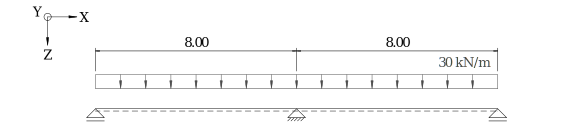
\includegraphics[keepaspectratio]{index_files/mediabag/../imgs/jag_makrosystem.pdf}}

}

\caption{\label{fig-jag_makrosystem}Statisches System mit schematischer
Stabunterteilung}

\end{figure}%

Die Abbildung~\ref{fig-jag_makrosystem} zeigt das System mit den
Doppelgelenken. Die effektive Stabeinteilung ist nicht dargestellt.

Das System ist für beide Stähle mit einer Streckenlast von 30 kN/m
belastet. Diese ist deutlich grösser gewählt als die analytisch
ermittelte.

\begin{figure}[H]

\centering{

\pandocbounded{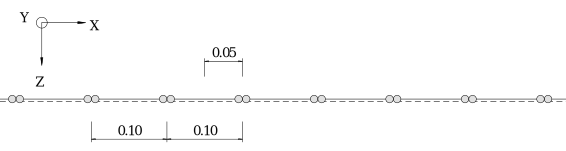
\includegraphics[keepaspectratio]{index_files/mediabag/../imgs/jag_makro_detail.pdf}}

}

\caption{\label{fig-jag_makro_detail}Detailansicht des statischen
Modells}

\end{figure}%

\subsection{Querschnittsmodellbildung}\label{querschnittsmodellbildung-1}

\subsubsection{Biegesteifigkeit}\label{biegesteifigkeit-2}

Es wird ausschliesslich das Biegeverhalten untersucht. Dazu wird eine
Querschnittsanalyse durchgeführt. Der Querschnitt ist bei steigender
Krümmung zu untersuchen. Mittels den Gleichgewichstbedingungen kann das
Biegemoment für die entsprechende Krümmung bestimmt werden. Dies führt
zu einer Momenten-Krümmungs-Beziehung.

Konkret ist in diesem Beispiel das Fliessmoment und der Biegewiderstand
vereinfacht an den folgenden Querschnitten bestimmt worden. Gezeigt in
der Abbildung~\ref{fig-jag_qs_fliessen} und
Abbildung~\ref{fig-jag_qs_widerstand}. Dabei erreicht der Stahl die
Fliessspannung, der Beton wird als vollständig plastifiziert angenommen.

\begin{figure}[H]

\centering{

\pandocbounded{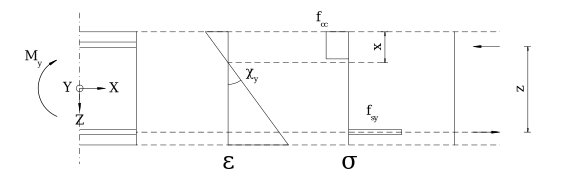
\includegraphics[keepaspectratio]{index_files/mediabag/../imgs/jag_qs_fliessen.pdf}}

}

\caption{\label{fig-jag_qs_fliessen}Querschnittsanalyse zur Bestimmung
des Fliessmoments und der Fliesskrümmung, Stahl erreicht Fliessgrenze,
Beton ist völlig plastifiziert}

\end{figure}%

Bei der Bestimmung der Bruchkrümmung fliesst das Zuggurtmodell mit ein.
Im Anhang~\ref{sec-zweifeldtraeger_anhang} ist die Berücksichtigung dazu
umfangreich aufgezeigt. Die Grundüberlegung liegt dabei, dass sich der
Beton ebenfalls am Spannungsabtrag beteiligt über die Verbundwirkung des
Betonstahls zum Beton. Dazu wird basierend auf dem Zuggurtmodell ein
Zugglied untersucht, speziell dessen Dehnungszustands. Anhand diesem
wird eine mittlere Dehnung ermittelt. Mit dieser mittleren Dehnung ist
hier die Bruchkrümmung ermittelt.

\begin{figure}[H]

\centering{

\pandocbounded{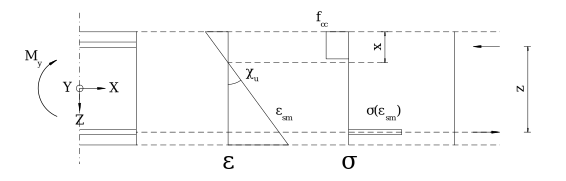
\includegraphics[keepaspectratio]{index_files/mediabag/../imgs/jag_qs_widerstand.pdf}}

}

\caption{\label{fig-jag_qs_widerstand}Querschnittsanalyse zur Bestimmung
des Biegewiderstands und der Bruchkrümmung, Stahl erreicht die Spannung
entsprechend der mittleren Dehnung des Zugglieds, Beton ist völlig
plastifiziert}

\end{figure}%

Die Krümmung gilt es mit der Einzugslänge, illustriert in der
Abbildung~\ref{fig-allg_feder}, zu multiplizieren um die Verdrehung zu
erhalten.

\subsubsection{Abbruchkriterium}\label{abbruchkriterium}

Es wird ein Abbruchkriterium definiert gemäss der Modellvorstellung in
Abbildung~\ref{fig-jag_plast_rot}. Dabei muss die Summe der relativen
Gelenkrotationen der Gelenke innerhalb der Länge des plastischen Gelenks
kleiner als das Rotationsvermögen sein.

\begin{equation}\phantomsection\label{eq-abbruchkriterium}{
\varphi_{max} \geq \sum_{i=1}^n \varphi_i
}\end{equation}

Dabei ist zwingend der ideal-plastische Verlauf am Ende der
Momenten-Verdrehungs-Beziehung zu hinterlegen, da einzelne Gelenke
innerhalb der plastischen Länge die Bruchverdrehung deutlich
überschreiten können. In der Summe diese jedoch kleiner als das
Rotationsvermögen sein müssen.

Die Abbildung~\ref{fig-jag_abbruchkrit} illustriert die plastische
Gelenklänge für das System.

\begin{figure}[H]

\centering{

\pandocbounded{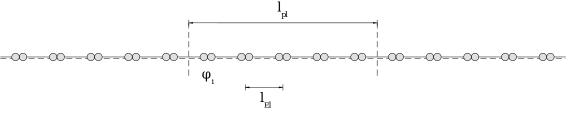
\includegraphics[keepaspectratio]{index_files/mediabag/../imgs/jag_abbruchkrit.pdf}}

}

\caption{\label{fig-jag_abbruchkrit}Definition des Abbruchkriteriums,
Gelenke innerhalb der Länge des plastischen Gelenks}

\end{figure}%

\subsection{Resultate}\label{resultate-1}

Das Anwendungsbeispiel wird mit den Berechnungsresultaten abgeschlossen.
Dazu ist das gesuchte Last-Verformungs-Diagramm in der
Abbildung~\ref{fig-jag_q_w} gezeigt. Aufgezeigt ist die analytische
Lösung und die numerische mittels dem nicht-linearen FE-Modell.

\begin{figure}[H]

\centering{

\pandocbounded{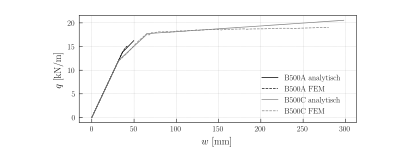
\includegraphics[keepaspectratio]{index_files/mediabag/../imgs/jag_q_w.pdf}}

}

\caption{\label{fig-jag_q_w}Last-Feldmittendurchbiegung-Diagramm für
beide Betonstähle, analytisch gelöst und mit der FEM-Lösung
nachgerechnet}

\end{figure}%

Die Verläufe für den kaltverformten Betonstahl B500A sind
deckungsgleich. Lediglich kleine Differenzen bei der prognostizierten
Traglast. Die analytische Lösung beschreibt eine um 5 \% höhere
Traglast. Da das FE-Modell lediglich eine Näherung beschreibt ist dieses
Resultat zufriedenstellend.

Die Verläufe für den naturharten Stahl B500C zeigen gleichbleibendes
Verhalten bis zu einer Verformung von 145mm. Exakt an diesem Punkt
erreicht das Gelenkpaar beim Auflager die Bruchkrümmung \(\varphi_u\).
Ab dann folgt im FE-Modell der ideal-plastische Bereich. Dies spiegelt
sich im Last-Verformungs-Verhalten wieder.

An diesem Verhalten lässt sich das Abbruchkriterium verdeutlichen. Wären
in den Momenten-Verdrehungs-Beziehungen keine ideal-plastischen Verläufe
hinterlegt, so läge die prognostizierte Verformung beim Erreichen der
Traglast lediglich bei 50\% der Verformung der analytischen Lösung.

Insgesamt weichen die numerischen Näherung weniger als 8\% von der
analytischen Lösung ab.

\subsubsection{Kaltverformter Stahl}\label{kaltverformter-stahl}

\begin{figure}[H]

\centering{

\pandocbounded{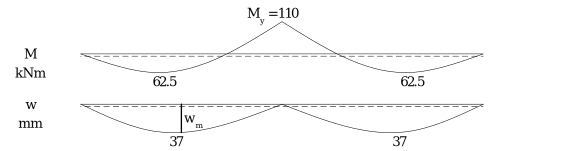
\includegraphics[keepaspectratio]{index_files/mediabag/../imgs/jag_b500a_lpa_0494.pdf}}

}

\caption{\label{fig-jag_b500a_lpa_0494}Resultate für den Lastfaktor
0.494}

\end{figure}%

\begin{figure}[H]

\centering{

\pandocbounded{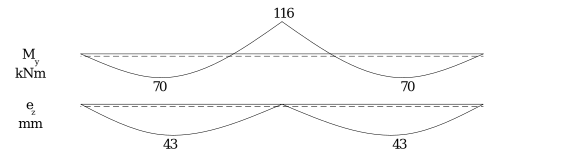
\includegraphics[keepaspectratio]{index_files/mediabag/../imgs/jag_b500a_lpa_0504.pdf}}

}

\caption{\label{fig-jag_b500a_lpa_0504}Resultate für den Lastfaktor
0.504}

\end{figure}%

Die relativen Gelenkrotationen in der Summe über die plastische Länge
entsprechen dem plastischen Rotationsvermögen.

\begin{figure}[H]

\centering{

\pandocbounded{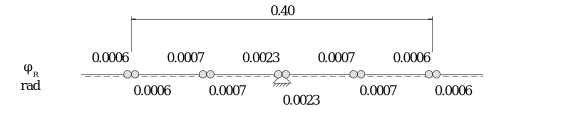
\includegraphics[keepaspectratio]{index_files/mediabag/../imgs/jag_b500a_lpa_0504_rot.pdf}}

}

\caption{\label{fig-jag_b500a_lpa_0504_rot}Relative Gelenkrotation für
den Lastfaktor 0.504}

\end{figure}%

\subsubsection{Naturharter Stahl}\label{naturharter-stahl}

\begin{figure}[H]

\centering{

\pandocbounded{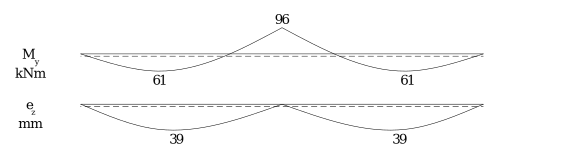
\includegraphics[keepaspectratio]{index_files/mediabag/../imgs/jag_b500c_lpa_0433.pdf}}

}

\caption{\label{fig-jag_b500c_lpa_0433}Resultate für den Lastfaktor
0.433}

\end{figure}%

\begin{figure}[H]

\centering{

\pandocbounded{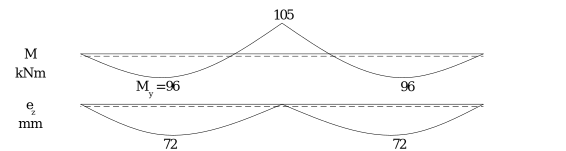
\includegraphics[keepaspectratio]{index_files/mediabag/../imgs/jag_b500c_lpa_0597.pdf}}

}

\caption{\label{fig-jag_b500c_lpa_0597}Resultate für den Lastfaktor
0.597}

\end{figure}%

\begin{figure}[H]

\centering{

\pandocbounded{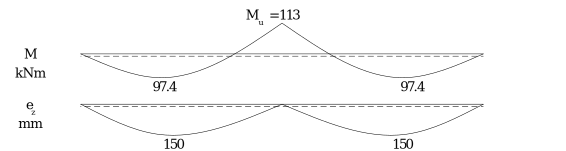
\includegraphics[keepaspectratio]{index_files/mediabag/../imgs/jag_b500c_lpa_0619.pdf}}

}

\caption{\label{fig-jag_b500c_lpa_0619}Resultate für den Lastfaktor
0.619}

\end{figure}%

\begin{figure}[H]

\centering{

\pandocbounded{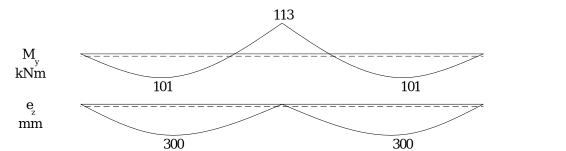
\includegraphics[keepaspectratio]{index_files/mediabag/../imgs/jag_b500c_lpa_0634.pdf}}

}

\caption{\label{fig-jag_b500c_lpa_0634}Resultate für den Lastfaktor
0.634}

\end{figure}%

Die relativen Gelenkrotationen in der Summe über die plastische Länge
entsprechen dem plastischen Rotationsvermögen.

\begin{figure}[H]

\centering{

\pandocbounded{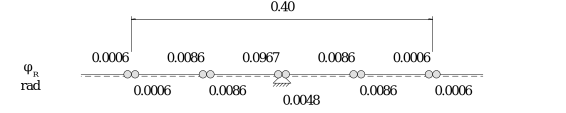
\includegraphics[keepaspectratio]{index_files/mediabag/../imgs/jag_b500c_lpa_0634_rot.pdf}}

}

\caption{\label{fig-jag_b500c_lpa_0634_rot}Relative Gelenkrotation für
den Lastfaktor 0.634}

\end{figure}%

\section{Fazit}\label{fazit}

Die dargestellen Resultate zeigen, dass sich die analytische Lösung
zuverlässig annähern lässt. Das Modell zeigt, dass die aufwändige
analytische Lösung, speziell die Systemanalye mit wenig
Modellierungsaufwand ersetzt werden kann. Zudem ist aufgezeigt, dass die
Steifigkeitsermittlung basierend auf den analytischen Modellen
problemlos in das FE-Modell integriert werden. Dies erhöht die
Nachvollziehbarkeit des Modells beträchtlich, da der Ingenieur die
Modellsteifigkeit direkt steuert und über meist bekannte Ansätze
berechnen kann.

\bookmarksetup{startatroot}

\chapter{Anwendung torsionsweicher
Trägerrost}\label{anwendung-torsionsweicher-truxe4gerrost}

Das vorangegangene Kapitel zeigt die Anwendung der Modellbildung an
einem zweidimensionalen Stabtragwerk. Mit dem Anwendungsbeispiel des
torsionsweichen Trägerrosts wird das Ziel verfolgt, ein
dreidimensionales System mit dem Stabsystem abzubilden.

\section{Aufgabenbeschrieb}\label{aufgabenbeschrieb-1}

Das folgende Beispiel stammt aus
{[}\citeproc{ref-marti_baustatik_2014}{4}{]}. In der
Abbildung~\ref{fig-trm_uebersicht} ist der Grundriss des Trägerrosts
dargestellt. Es handelt sich um insgesamt 16 torsionsweiche Stäbe,
welche an den Enden eingespannt sind.

\begin{figure}[H]

\centering{

\pandocbounded{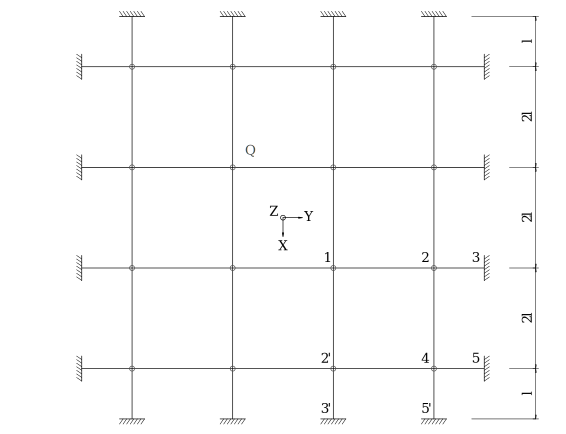
\includegraphics[keepaspectratio]{index_files/mediabag/../imgs/trm_uebersicht.pdf}}

}

\caption{\label{fig-trm_uebersicht}Grundriss des torsionsweichen
Trägerrosts, neugezeichnet nach
{[}\citeproc{ref-marti_baustatik_2014}{4}{]}}

\end{figure}%

Im Beispiel wird eine analytische Lösung zur Traglast aufgezeigt. Das
Ziel ist es, mittels dem nicht-linearen FE-Modell eine numerische Lösung
des unteren Grenzwerts der Traglast zu erhalten.

\section{Analytische Lösung}\label{analytische-luxf6sung-1}

Die Analytische Lösung basiert auf dem Traglastverfahren. Mittels einem
zulässigen Mechanismus wird ein oberer Grenzwert der Traglast
hergeleitet. In der Abbildung~\ref{fig-trm_schnitt} sind zwei Stäbe
dargestellt. Aus symmetriegründen lässt sich der obere Grenzwert des
gesamten Trägerrosts anhand dieser Darstellung ermitteln.

\begin{figure}[H]

\centering{

\pandocbounded{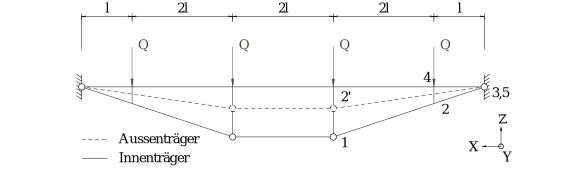
\includegraphics[keepaspectratio]{index_files/mediabag/../imgs/trm_schnitt.pdf}}

}

\caption{\label{fig-trm_schnitt}Schnitt des torsionsweichen Trägerrosts,
mit dem angenommenen Mechanismus für den Innen- und Aussenträger}

\end{figure}%

Die äussere Arbeit \(W_a\) des dargestellten Systems in
Abbildung~\ref{fig-trm_schnitt} beträgt dabei für die am Rand gelegenen
Stäbe (Punkte 2'45):

\[
W_{a,2'45} = 4 \cdot \left( Q \cdot \frac{1}{3} + Q \cdot \frac{1}{9} \right)
\]

Und für die Innenträger:

\[
W_{a,123} = 4 \cdot \left( Q \cdot 1 + Q \cdot \frac{1}{3} \right)
\]

Sowie beträgt die innere Arbeit:

\[
W_i = 8 \cdot \left(M_u' + M_u\right) \cdot \left(\frac{1}{3l} +\frac{1}{9l}\right)
\]

Durch das abschliessende Gleichsetzen der Arbeiten und das Lösen nach
\(Q\) folgt der obere Grenzwert der Traglast zu:

\[
Q = \frac{M_u + M_u'}{2 \cdot l}
\]

Die Plastizitätskontrolle ist in der Abbildung~\ref{fig-trm_schnitt_my}
und Abbildung~\ref{fig-trm_schnitt_vz} gezeigt. Dabei wird eine
Lastverteilung von je einer Hälfte \(Q\) in \(x\) und \(y\) Richtung
angenommen. Welche sich nach vollständigen Umlagern der Biegemomente
einstellt.

\begin{figure}[H]

\centering{

\pandocbounded{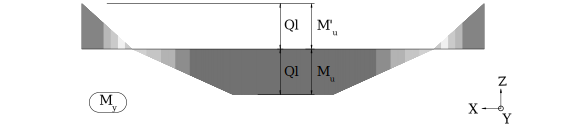
\includegraphics[keepaspectratio]{index_files/mediabag/../imgs/trm_schnitt_my.pdf}}

}

\caption{\label{fig-trm_schnitt_my}Plastizitätskontrolle anhand der
Schnittgrössen der Biegemomente}

\end{figure}%

\begin{figure}[H]

\centering{

\pandocbounded{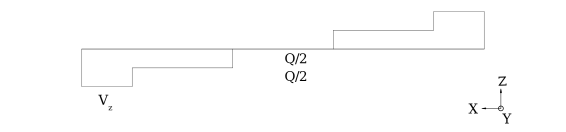
\includegraphics[keepaspectratio]{index_files/mediabag/../imgs/trm_schnitt_vz.pdf}}

}

\caption{\label{fig-trm_schnitt_vz}Plastizitätskontrolle anhand der
Schnittgrössen der Querkräfte}

\end{figure}%

Aus der Plastizitätskontrolle geht heraus, dass der Biegewiderstand
nirgends überschritten wird, somit deckt sich der untere und obere
Grenzwert der Traglast, sprich die Traglast \(Q_u\) wurde gefunden.

\[
Q_u = \frac{M_u + M_u'}{2 \cdot l}
\]

\section{NLFE-Modell}\label{nlfe-modell-1}

Abschliessend wird die analytische Lösung mit der numerischen Lösung
verglichen. Dabei wird das nicht-lineare FE-Modell erstellt. Zunächst
sind die Variablen mit numerischen Werten zu substituieren:

\[
\begin{aligned}
l& = 1.0 \ \mathrm{m} \quad & M_{u}& = 100 \ \mathrm{kN} \cdot \mathrm{m} \quad & {M}'_{u}& = 100 \ \mathrm{kN} \cdot \mathrm{m} \end{aligned}
\]

Die geforderte Traglast des Systems liegt gemäss der analytischen Lösung
für die gewählten Werte bei:

\[
\begin{aligned}
Q_{u}& = \frac{M_{u} + {M}'_{u}}{2 \cdot l} = 100.0 \ \mathrm{kN} \end{aligned}
\]

Die Modellierte Einzellast beträgt.

\[
\begin{aligned}
Q& = 120 \ \mathrm{kN} \quad &  \quad &  
 \end{aligned}
\]

\subsection{Makromodellbildung}\label{makromodellbildung}

Der Trägerrost wurde mittels dem Federmodell nachmodelliert. Dabei sind
biegestarre, jedoch torsionsweiche Stäbe mittels Stabendgelenken
gekoppelt. Dargestellt in der Abbildung~\ref{fig-trm_geom}.

\begin{figure}[H]

\centering{

\pandocbounded{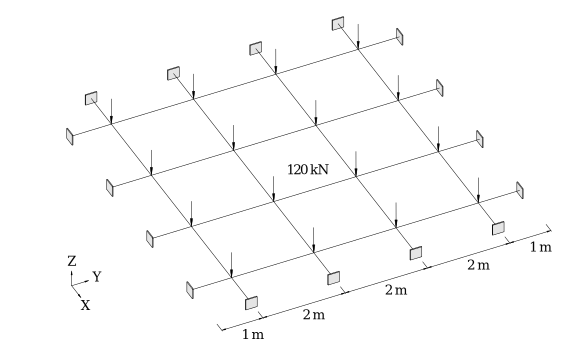
\includegraphics[keepaspectratio]{index_files/mediabag/../imgs/trm_system.pdf}}

}

\caption{\label{fig-trm_geom}Statisches Modell in AxisVM des
Trägerrosts}

\end{figure}%

\begin{figure}[H]

\centering{

\pandocbounded{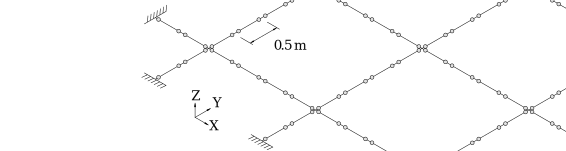
\includegraphics[keepaspectratio]{index_files/mediabag/../imgs/trm_detail_system.pdf}}

}

\caption{\label{fig-trm_detail_system}Detailausschnitt des Trägerrosts
mit Gelenken und vermasster Elementlänge}

\end{figure}%

\subsection{Mikromodellbildung}\label{mikromodellbildung}

\subsubsection{Biegeverhalten}\label{biegeverhalten}

\begin{figure}[H]

\centering{

\pandocbounded{\includegraphics[keepaspectratio]{index_files/mediabag/../imgs/trm_gelenkdef.pdf}}

}

\caption{\label{fig-trm_gelenkdef}Ideal-plastisches
Momenten-Verdrehungs-Verhalten der Gelenke}

\end{figure}%

Den Gelenken wurde die Defintion gemäss
Abbildung~\ref{fig-trm_gelenkdef} hinterlegt. Dabei wurde der
Biegewiderstand in positiver und negativer Dimension angesetzt, ab dem
Erreichen des Biegewiderstands fliesst das Gelenk. Dies führt dazu, dass
sich die Biegemomente umlagern, sprich der Biegewiderstand auch in
Trägermitte erreicht werden kann.

\subsubsection{Abbruchkriterium}\label{abbruchkriterium-1}

Nicht-Konvergenz

\subsection{Resultate}\label{resultate-2}

Bei der Traglastermittlung des Systems ist das Rotationsvermögen des
Systems von keiner bedeutung. Die Traglast stellt sich bei einer
vollständigen Umlagerung sämtlicher Biegemomente ein. Die folgenden
Abbildungen zeigen die Verteilung der Biegemomente und der Querkräfte im
Trägerrost, ermittelt mit dem NLFE-Modell.

Die ersten Gelenke bei den innenliegenden Stäbe bilden sich bei
folgender Last.

\[
\begin{aligned}
Q_{1}& = Q \cdot 0.493 = 59.16 \ \mathrm{kN} \quad &  \quad &  
 \end{aligned}
\]

Dazu ist in der Abbildung~\ref{fig-trm_1} die Zustandslinien der
Biegemomente gezeigt.

\begin{figure}[H]

\centering{

\pandocbounded{\includesvg[keepaspectratio]{../imgs/trm_1.svg}}

}

\caption{\label{fig-trm_1}Biegemomente des Trägerrosts, erste plastische
Gelenke entstehen bei der Lagerung der Innenträger}

\end{figure}%

Bei den Aussenträgern bilden sich plastische Gelenke bei folgender
Laststufe.

\[
\begin{aligned}
Q_{2}& = Q \cdot 0.758 = 90.96 \ \mathrm{kN} \quad &  \quad &  
 \end{aligned}
\]

Die folgenden beiden Abbildungen zeigen die Zustandslinien der
Biegemomente und der Querkräfte. Der Biegewiderstand ist bei sämtlichen
Auflagernpunkten erreicht.

\begin{figure}[H]

\centering{

\pandocbounded{\includesvg[keepaspectratio]{../imgs/../imgs/trm_2.svg}}

}

\caption{\label{fig-trm_2}Biegemomente des Trägerrosts, plastische
Gelenke entstehen bei der Lagerung der Aussenträger}

\end{figure}%

Die Bildung des Fliessgelenks im Feld bei den Innenträgern liegt nahe
bei der vorherigen Laststufe.

\[
\begin{aligned}
Q_{3}& = Q \cdot 0.781 = 93.72 \ \mathrm{kN} \quad &  \quad &  
 \end{aligned}
\]

Die Zustandslinien dazu sind folgend gezeigt. Es zeigt sich, dass in
Feldmitte der Biegewiderstand erreicht ist.

\begin{figure}[H]

\centering{

\pandocbounded{\includesvg[keepaspectratio]{../imgs/trm_3.svg}}

}

\caption{\label{fig-trm_3}Biegemomente des Trägerrosts, plastische
Gelenke entstehen im Feld der Innenträger}

\end{figure}%

Abschliessend gibt es ein Konvergenzproblem bei folgender Laststufe.

\[
\begin{aligned}
Q_{4}& = Q \cdot 0.832 = 99.84 \ \mathrm{kN} \quad &  \quad &  
 \end{aligned}
\]

Die Zustandslinien der Biegemomente zeigen ein Erreichen des
Biegewiderstands im Feld der Aussenträger. Die Traglast ist erreicht.

\begin{figure}[H]

\centering{

\pandocbounded{\includesvg[keepaspectratio]{../imgs/trm_4.svg}}

}

\caption{\label{fig-trm_4}Querkräfte des Trägerrosts, plastische Gelenke
entstehen im Feld der Aussenträger}

\end{figure}%

\section{Fazit}\label{fazit-1}

\begin{itemize}
\tightlist
\item
\end{itemize}

\bookmarksetup{startatroot}

\chapter{Anwendung Quadratplatte}\label{anwendung-quadratplatte}

Die vorgängige Anwendung des torsionsweichen Trägerrostes hat gezeigt,
dass sich der untere Grenzwert Traglast zuverlässig mithilfe des
NLFE-Modells (nichtlineares Finite-Elemente-Modell) bestimmen lässt. Der
Modellierungsaufwand bleibt dabei gering, da das verwendete Mikromodell
lediglich ein ideal-plastisches Biegeverhalten abbildet.

In diesem Kapitel mit Trägerrost Traglast einer Platte. Schritt von
Trägerrost zu Plattentragwerk bedeutet Berücksichtigung Drillmomente.
Die Randbedingungen der Platte sind so gewählt, dass der obere und der
untere Grenzwert zusammenfallen.

\section{Aufgabenbeschrieb}\label{aufgabenbeschrieb-2}

Die Abbildung~\ref{fig-quad_aufgabenstellung} zeigt eine Quadratplatte
mit einer konstanten Flächenlast belastet. Die Platte ist an allen
Rändern gelenkig gelagert.

\begin{figure}[H]

\centering{

\pandocbounded{\includegraphics[keepaspectratio]{index_files/mediabag/../imgs/quad_aufgabenstellung.pdf}}

}

\caption{\label{fig-quad_aufgabenstellung}Quadratplatte mit
gleichmässiger Flächenlast. Dazu sind Masslinien und Auflager gezeigt}

\end{figure}%

Das Ziel ist es die Traglast des Systems analytisch zu bestimmen.
Abschliessend ist dies mit der Lösung des NLFE-Modells zu vergleichen.
Der Biegewiderstand der Platte entspricht:

\[
\begin{aligned}
m_{u}& = 100.0 \ \frac{\mathrm{kNm}}{\mathrm{m}} \quad &  \quad &  
 \end{aligned}
\]

\section{Analytische Lösung}\label{analytische-luxf6sung-2}

Der obere Grenzwert der analytischen Lösung basiert auf der
Fliessgelenklinienmethode. Die Fliessgelenke sind über die Fliessfigur
in Abbildung~\ref{fig-quad_fliessfigur_norm} bestimmt. Die Fliessfigur
zeigt eine Interaktion zwischen Biege- und Drillmomenten. Der maximale
Drillmomentenwiderstand beschreibt die
Gleichung~\ref{eq-drill_fliessgelenk}.

\begin{equation}\phantomsection\label{eq-drill_fliessgelenk}{
m_{xy,max} = \frac{1}{2} \sqrt{(m_x + m'_x) (m_y + m'_y)}
}\end{equation}

Anhand eines gewählten Mechanismus kann über das Gleichsetzen der
inneren und äusseren Arbeit der obere Grenzwert der Traglast bestimmt
werden.In {[}\citeproc{ref-marti_baustatik_2014}{4}{]} ist die Methode
detailliert beschrieben.

\begin{figure}[H]

\centering{

\pandocbounded{\includegraphics[keepaspectratio]{index_files/mediabag/../imgs/quad_fliessfigur_norm.pdf}}

}

\caption{\label{fig-quad_fliessfigur_norm}Fliessfigur der
Fliessgelenklinienmethode im \(m_x , m_y, m_{xy}\)-Raum}

\end{figure}%

Das Kapitel 25.5.3 aus {[}\citeproc{ref-marti_baustatik_2014}{4}{]}
zeigt die Bestimmung der Traglast einer einfach gelagerten
Rechteckplatte. Der Mechanismus, sprich die Anordnung der
Fliessgelenklinien in der Platte, zeigt die
Abbildung~\ref{fig-quad_rechteck_allg}.

\begin{figure}[H]

\centering{

\pandocbounded{\includegraphics[keepaspectratio]{index_files/mediabag/../imgs/quad_rechteck_allg.pdf}}

}

\caption{\label{fig-quad_rechteck_allg}Fliessgelenklinien eine einfach
gelagerten Rechteckplatte, neugezeichnet nach
{[}\citeproc{ref-marti_baustatik_2014}{4}{]}}

\end{figure}%

Mittels den Momentenansätzen, beschrieben in
{[}\citeproc{ref-marti_baustatik_2014}{4}{]}, lassen sich die
Gleichgewichtsbedingungen und die statischen Randbedingungen erfüllen,
einen unteren Grenzwert der Traglast ermitteln.

Die Anwendung beider Methoden auf die Rechteckplatte liefert die
folgende Eingrenzung der Traglast:

\[
8(1+ \beta + \beta^2) \leq \frac{q_u b^2}{m_u} \leq \frac{24}{(\sqrt{3+\beta^2} - \beta)^2}
\]

dabei entspricht \(\beta\) dem Verhältnis der Seitenlängen:

\[
\beta = \frac{b}{a}
\]

Für die Quadratplatte ist \(a = b\) anzusetzen. Dies führt zu dem
Mechanismus gemäss der
Abbildung~\ref{fig-quad_quadrat_fliessgelenklinien}.

\begin{figure}[H]

\centering{

\pandocbounded{\includegraphics[keepaspectratio]{index_files/mediabag/../imgs/quad_quadrat_fliessgelenklinien.pdf}}

}

\caption{\label{fig-quad_quadrat_fliessgelenklinien}Fliessgelenklinien
der einfach gelagerten Quadratplatte}

\end{figure}%

Die folgende Beziehung beschreibt die Eingrenzung der Traglast der
einfach gelagerten Quadratplatte.

\[
\frac{24 m_u}{a^2} \leq q_u \leq \frac{24 m_u}{a^2} 
\]

Es ist ersichtlich, dass die Grenzen zusammenfallen. Die Traglast ist
somit eindeutig bestimmt. Mit den gewählten Abmessungen und dem
Biegewiderstand folgt die Traglast zu:

\[
\begin{aligned}
a& = 10 \ \mathrm{m} \quad & q_{u}& = \frac{24 \cdot m_{u}}{a^{2}} = 24.0 \ \frac{\mathrm{kN}}{\mathrm{m}^{2}} \end{aligned}
\]

\section{NLFE-Modell}\label{nlfe-modell-2}

Nach der Bestimmung der analytischen Traglast zeigt der folgende
Abschnitt die Modellbildung des nicht-linearen FE-Modells. Es ist
zwischen Makro- und Mikromdellbildung unterschieden.

\subsection{Makromodellbildung}\label{makromodellbildung-1}

Das System, sprich das Makromodell ist in der \textbf{?@fig-quad\_makro}
gezeigt. Gezeigt sind der Trägerrost, Stabanfang- und Endgelenke,
Auflager und Knotenlasten. Die Gelenke sind gemäss der
Modellierungsstrategie angeordnet. Die Elementlänge entspricht:

\[
\begin{aligned}
l_{El}& = 1.0 \ \mathrm{m} \end{aligned}
\]

Knotenlasten durch die Flächenlast in Abhängigkeit der Einzugsfläche
bestimmt. Bei den Randknoten ist die Hälfte anzusetzen.

\[
\begin{aligned}
Q& = 50 \ \mathrm{kN} \quad &  \quad &  
 \end{aligned}
\]

Die Knotenlast ist grosszügig grösser als die Traglast gewählt. Aufgrund
des gewählten Abbruchkriteriums stellt sich ein Lastfaktor ein. Mit
diesem Lastfaktor lässt sich die Traglast bestimmen. Wichtig ist
lediglich die Lastaufteilung.

\begin{figure}[H]

\centering{

\pandocbounded{\includesvg[keepaspectratio]{../imgs/quad_system.svg}}

}

\caption{\label{fig-quad_system}Trägerrostmodell}

\end{figure}%

\begin{figure}[H]

\centering{

\pandocbounded{\includesvg[keepaspectratio]{../imgs/quad_lasten.svg}}

}

\caption{\label{fig-quad_lasten}Detailausschnitt eines Ecks,
Knotenlasten und Knotenlager sind dargestellt}

\end{figure}%

\subsection{Mikromodellbildung}\label{mikromodellbildung-1}

Die Mikromodellbildung unterscheidet zwischen dem Biegeverhalten und dem
Torsionsverhalten.

\subsubsection{Biegeverhalten}\label{biegeverhalten-1}

Das Biegeverhalten ist mit einer Momenten-Verdrehungs-Beziehung
definiert. Der Biegewiderstand des Stabs beträgt:

\[
\begin{aligned}
M_{u}& = m_{u} \cdot l_{El} = 100.0 \ \mathrm{kNm} \end{aligned}
\]

Die Momenten-Verdrehungs-Beziehung zeigt die
Abbildung~\ref{fig-quad_gelenkdef_biegung}. Das ideal-plastische
Verhalten beschreibt ein ideal weiches Verhalten beim Erreichen des
Biegewiderstands.

\begin{figure}[H]

\centering{

\pandocbounded{\includegraphics[keepaspectratio]{index_files/mediabag/../imgs/trm_gelenkdef.pdf}}

}

\caption{\label{fig-quad_gelenkdef_biegung}ideal-plastisches
Momenten-Verdrehungs-Verhalten}

\end{figure}%

Das Verhalten ist gemäss der Gleichung~\ref{eq-dreidim_gelenkfunktionen}
der Biegung um die lokale Y-Achse des Stabs zuzuordnen. Zudem lässt sich
das Verhalten lediglich numerisch annähern. Es verbleibt eine elastische
und eine plastische Steifigkeit. Die letztere ist minimal zu wählen.

\subsubsection{Torsionsverhalten}\label{torsionsverhalten}

Das Torsionsverhalten des Stabs beschreibt das Drillverhalten des
Plattenelements. Eine anzustrebende Interaktion zwischen Biegung und
Drillung lässt sich nicht modellieren. Vereinfacht ist das
Torsionsverhalten gleich dem Biegeverhalten modelliert.

Gemäss der Gleichung~\ref{eq-dreidim_gelenkfunktionen} ist in lokaler
X-Richtung ein Momenten-Verdrehungs-Verhalten gemäss der
Abbildung~\ref{fig-quad_gelenkdef_biegung} hinterlegt. Der
Torsionswiderstand beträgt dabei:

\[
\begin{aligned}
M_{u xy}& = M_{u} = 100.0 \ \mathrm{kNm} \end{aligned}
\]

Das modellierte Verhalten lässt sich an der Fliessfigur illustrieren.
Die Abbildung~\ref{fig-quad_fliessfigur_axis} zeigt die Fliessfigur des
Trägerrosts. Die Darstellung ist schematisch für sich unterscheidende
positive und negative Biegewiderstände. Grau hinterlegt ist die
Fliessfigur der Fliessgelenklinienmethode.

\begin{figure}[H]

\centering{

\pandocbounded{\includegraphics[keepaspectratio]{index_files/mediabag/../imgs/quad_fliessfigur_axis.pdf}}

}

\caption{\label{fig-quad_fliessfigur_axis}Fliessfigur des Trägerrosts im
\(m_x , m_y, m_{xy}\)-Raum}

\end{figure}%

Die Darstellung verdeutlicht, dass bei hohen Biegemomenten und zugleich
grosser Torsionsbeanspruchung das Tragverhalten überschätzt überschätzt
wird im Vergleich mit der Fliessgelenklinienmethode.

\subsubsection{Abbruchkriterium}\label{abbruchkriterium-2}

Abschliessend ist das Abbruchkriterium zu definieren. Die Berechnung ist
abzubrechen, sobald keine Konvergenz mehr eintritt. Ab einer gewissen
Anzahl an Fliessgelenken lässt sich die Last nicht mehr steigern. Es
stellt sich ein asymptotischer Verlauf im Last-Verformungs-Diagramm ein.
Dargestellt ist ein schematisches Verhalten in der
Abbildung~\ref{fig-quad_abbruch}.

\begin{figure}[H]

\centering{

\pandocbounded{\includegraphics[keepaspectratio]{index_files/mediabag/../imgs/quad_abbruch.pdf}}

}

\caption{\label{fig-quad_abbruch}Last-Verformungs-Verhalten des Systems
bei der Ermittlung der Traglast, schematisch dargestellt}

\end{figure}%

\subsection{Resultate}\label{resultate-3}

Das Last-Verformungs-Verhalten in der Abbildung~\ref{fig-quad_Q_w} zeigt
das Systemverhalten. Es zeigt einen asymptotischen Verlauf beim
Erreichen der Traglast. Die Verformung ist nicht aussagekräftig. Diese
ist abhängig von der gewählten elastischen Steifigkeit.

\begin{figure}[H]

\centering{

\pandocbounded{\includegraphics[keepaspectratio]{index_files/mediabag/../imgs/quad_Q_w.pdf}}

}

\caption{\label{fig-quad_Q_w}Last-Verformungs-Verhalten des Systems.
Asymptotischer Verlauf bei 25 kN}

\end{figure}%

Der Konvergenzabbruch stellt sich bei folgendem Lastparameter ein:

\[
\begin{aligned}
Lpa& = 0.505 \quad &  \quad &  
 \end{aligned}
\]

Bezogen auf die Knotenlast folgt:

\[
\begin{aligned}
Q_{u}& = Lpa \cdot Q = 25.25 \ \mathrm{kN} \quad &  \quad &  
 \end{aligned}
\]

Und abschliessend verteilt auf die Lasteinzugsfläche folgt:

\[
\begin{aligned}
A_{Einzug}& = l_{El}^{2} = 1.0 \ \mathrm{m}^{2} \quad & q_{u NLFE}& = \frac{Q_{u}}{A_{Einzug}} = 25.25 \ \frac{\mathrm{kN}}{\mathrm{m}^{2}} \quad &  
 \end{aligned}
\]

Die Zustandslinien der Biegemomente direkt aus AxisVM-X7 ist in der
gezeigt. Die Darstellung zeigt die sich bildenden plastischen Gelenke in
rot.

Vergleicht man die analytische Lösung der Traglast mit dem numerischen
unteren Grenzwert, so zeigt sich eine Abweichung von 5\%.

\[
\begin{aligned}
\eta_{q u}& = \frac{q_{u NLFE}}{q_{u}} = 105.21 \ \mathrm{\%} \quad &  \quad &  
 \end{aligned}
\]

Dabei ist hervorzuheben, dass die numerische Lösung eine grössere
Traglast als der obere Grenzwert der analytischen Lösung liefert. Dies
ist auf zwei Beweggründe zurückzuführen. Zunächst handelt es sich um
eine Näherung. Die Elementlänge ist relativ gross gewählt. Des Weiteren
sind die Systeme unterschiedlich. Der untere Grenzwert des Trägerrosts
wäre mit dem oberen Grenzwert des Trägerrost zu vergleichen, nicht mit
dessen des Plattentragwerks. Somit verletzt die Lösung keineswegs die
Grundsätze der Grenzwerte des Traglastverfahrens.

\begin{figure}[H]

\centering{

\pandocbounded{\includesvg[keepaspectratio]{../imgs/quad_1.svg}}

}

\caption{\label{fig-quad_1}Verlauf der Biegemomente bei der Laststufe
xx}

\end{figure}%

\begin{figure}[H]

\centering{

\pandocbounded{\includesvg[keepaspectratio]{../imgs/quad_4.svg}}

}

\caption{\label{fig-quad_4}Verlauf der Torsionsmomente bei der Laststufe
xx}

\end{figure}%

\begin{figure}[H]

\centering{

\pandocbounded{\includesvg[keepaspectratio]{../imgs/quad_2.svg}}

}

\caption{\label{fig-quad_2}Verlauf der Biegemomente bei der Laststufe
xx}

\end{figure}%

\begin{figure}[H]

\centering{

\pandocbounded{\includesvg[keepaspectratio]{../imgs/quad_5.svg}}

}

\caption{\label{fig-quad_5}Verlauf der Torsionsmomente bei der Laststufe
xx}

\end{figure}%

\begin{figure}[H]

\centering{

\pandocbounded{\includesvg[keepaspectratio]{../imgs/quad_3.svg}}

}

\caption{\label{fig-quad_3}Verlauf der Biegemomente bei der Laststufe
xx}

\end{figure}%

\begin{figure}[H]

\centering{

\pandocbounded{\includesvg[keepaspectratio]{../imgs/quad_6.svg}}

}

\caption{\label{fig-quad_6}Verlauf der Torsionsmomente bei der Laststufe
xx}

\end{figure}%

\section{Fazit}\label{fazit-2}

\bookmarksetup{startatroot}

\chapter{Versuchsnachrechnung
Zweifeldplatte}\label{versuchsnachrechnung-zweifeldplatte}

Die Anwendung an der Quadratplatte hat gezeigt, dass mit dem Trägerrost
das Tragverhalten von Plattentragwerken abgebildet werden kann, sofern
das Drilltragverhalten modelliert wird. Die Versuchsnachrechnung einer
Zweifeldplatte erweitert die Anwendung des Modells auf ein reales
Beispiel. Das Ziel ist es das Last-Verformungs-Verhalten und die
Traglast der Zweifeldplatte mit dem NLFE-Modell abzubilden.

Das Kapitel zeigt den Versuchsbeschrieb, Die Makro- und
Mikromodellbildung und die Resultate. In der Mikromodellbildung ist die
Ermittlung des Biegetragverhaltens und des Torsionstragverhaltens
gezeigt, sowie das Abbruchkriterium. Als Abschluss des Kapitels dient
ein Fazit.

\section{Versuchsbeschrieb}\label{versuchsbeschrieb}

Die Zweifeldplatte entstammt aus
{[}\citeproc{ref-thoma_plattenversuche_2010}{5}{]}. Es handelt sich um
eine einfach gelagerte Platte. Belastet ist diese mit Zugstangen,
verankert im Aufspannboden an Hydraulikzylindern, in den jeweiligen
Feldbereichen. Eine Darstellung des Versuchsaufbaus zeigt die
Abbildung~\ref{fig-tho_aufbau_iso}.

\begin{figure}[H]

\centering{

\pandocbounded{\includegraphics[keepaspectratio]{index_files/mediabag/../imgs/tho_aufbau_iso.pdf}}

}

\caption{\label{fig-tho_aufbau_iso}Isometrische Ansicht des
Versuchsaufbaus, dargestellt sind die Platte, die Lagerung, die
Krafteinleitung mittels den Zugstangen, ein Ringbalken unterhalb der
Lagerung und Mauerwerkswände als Auflager der Ringbalken}

\end{figure}%

Der Grundriss und die Längsansicht zeigt die
Abbildung~\ref{fig-tho_aufbau_gr}. Diese zeigt die Position der
Gleitlager, die Position der Zugstangen und die Hauptabmessungen der
Platte.

\begin{figure}[H]

\centering{

\pandocbounded{\includegraphics[keepaspectratio]{index_files/mediabag/../imgs/tho_aufbau_gr.pdf}}

}

\caption{\label{fig-tho_aufbau_gr}Grundriss und Längsansicht,
Lasteineinleitung, Lagerposition und die Plattenabmessungen sind
vermasst}

\end{figure}%

Zum Monitoring des Körpers sind Wegaufnehmer unterhalb der Platte
platziert worden. Die Anordnung ist in der
Abbildung~\ref{fig-tho_messung_gr} gezeigt. Es wurde nach dem Einbringen
des Körpers eine Nullmessung durchgeführt. Die gemessenen Verformungen
entsprechen somit ausschliesslich der Deformation des Körpers durch die
Belastung mit den Hydraulikzylindern.

\begin{figure}[H]

\centering{

\pandocbounded{\includegraphics[keepaspectratio]{index_files/mediabag/../imgs/tho_messung_gr.pdf}}

}

\caption{\label{fig-tho_messung_gr}Position der Wegaufnehmer, vermasst
auf Lagerachsen}

\end{figure}%

Der Versuch wurde bis zum Bruch gefahren. Nach dem Einbringen der Platte
wurde die Last gleichmässig belastet, die Hydraulikzylinder wiesen bei
sämtlichen Laststufen die jeweils gleiche Lastintensität auf. Der Bruch
trat durch das Zerreissen der oberen Längsbewehrung im mittleren
Auflagerberich ein.

\subsection{Berechnungsgrössen}\label{berechnungsgruxf6ssen}

Im Folgenden sind die Berechnungsgrössen zum Betonstahl, Beton und der
Geometrie aufgelistet. Diese sind allesamt aus dem Versuchsbericht
{[}\citeproc{ref-thoma_plattenversuche_2010}{5}{]}.

\subsubsection{Betonstahl}\label{betonstahl}

Die Platte ist kreuzweise mit einer Biegebewehrung mit Durchmesser 10 mm
und einer 150 mm Teilung versehen. Dies gilt für die obere und untere
Bewehrung. Am Rand sind Abschlussbügel verlegt. Zudem ist über dem
Mittelauflager eine Querkraftbewehrung eingelegt. Die
Abbildung~\ref{fig-tho_biegebewehrung_iso} zeigt lediglich die
Biegebewehrung.

\begin{figure}[H]

\centering{

\pandocbounded{\includegraphics[keepaspectratio]{index_files/mediabag/../imgs/tho_biegebewehrung_iso.pdf}}

}

\caption{\label{fig-tho_biegebewehrung_iso}Biegebewehrung der Platte}

\end{figure}%

Daraus lassen sich die folgenden Parameter der Biegebewehrung ableiten:

\[
\begin{aligned}
\oslash_{s}& = 10 \ \mathrm{mm} \quad & s& = 150 \ \mathrm{mm} \quad & a_{s}& = \frac{\oslash_{s}^{2} \cdot \pi}{4 \cdot s} = 523.6 \ \frac{\mathrm{mm}^{2}}{\mathrm{m}} \end{aligned}
\]

Die Eigenschaften des Betonstahls sind experimentell mit Zugversuchen
bestimmt worden. Dabei sind Angaben zu der Zugfestigkeit, Fliessgrenze,
Elastizitätsmodul, Fliessdehnung und Bruchdehnung aus dem Bericht
entnommen:

\[
\begin{aligned}
f_{su}& = 558.6 \ \frac{\mathrm{N}}{\mathrm{mm}^{2}} \quad & f_{sy}& = 445.6 \ \frac{\mathrm{N}}{\mathrm{mm}^{2}} \quad & E_{s}& = 196.5 \ \frac{\mathrm{kN}}{\mathrm{mm}^{2}} \\ 
\varepsilon_{sy}& = \frac{f_{sy}}{E_{s}} = 2.27 \ \mathrm{‰} \quad & \varepsilon_{su}& = 80.8 \ \mathrm{‰} \quad &  
 \end{aligned}
\]

\subsubsection{Beton}\label{beton}

Ebenso wurde der verwendete Beton experimentell untersucht. Im Bericht
sind Angaben zu der Zylinderdruckfestigkeit und dem Elastizitätsmodul
beschrieben.

\[
\begin{aligned}
f_{cc}& = 28.61 \ \frac{\mathrm{N}}{\mathrm{mm}^{2}} \quad & E_{c}& = 22.9 \ \frac{\mathrm{kN}}{\mathrm{mm}^{2}} \quad &  
 \end{aligned}
\]

Basierend auf empirischen Ansätzen lässt sich eine Bauteilfestigkeit und
die Betonzugfestigkeit bestimmen. Zudem ist die Annahme der
Betonbruchstauchung aufgezeigt.

\[
\begin{aligned}
f_{c}& = 2.7 \cdot f_{cc}^{\frac{2}{3}} = 25.26 \ \frac{\mathrm{N}}{\mathrm{mm}^{2}} \quad & f_{ct}& = 0.3 \cdot f_{cc}^{\frac{2}{3}} = 2.81 \ \frac{\mathrm{N}}{\mathrm{mm}^{2}} \quad & \varepsilon_{cu}& = 5.0 \ \mathrm{‰} \end{aligned}
\]

\subsubsection{Geometrie}\label{geometrie}

Die Plattenstärke und die Bewehrungsüberdeckung sind die folgenden:

\[
\begin{aligned}
h& = 200 \ \mathrm{mm} \quad & c_{nom}& = 20 \ \mathrm{mm} \quad &  
 \end{aligned}
\]

\subsection{Versuchsergebnisse}\label{versuchsergebnisse}

Aus dem Versuchsbericht geht eine Traglast und ein
Last-Verformungs-Diagramm hervor. Die Traglast beträgt 978 kN pro Feld.
Dies entspricht der Summe der einzelnen Hydraulikzylindern pro Feld.
Folglich beträgt die Traglast pro Zylinder:

\[
\begin{aligned}
Q_{u}& = \frac{978}{12} = 81.5 \ \mathrm{kN} \quad &  \quad &  
 \end{aligned}
\]

Das Last-Verformungs-Diagramm zeigt die Abbildung~\ref{fig-tho_res_V10}.
Auf der Ordinate ist die Summe der Einzelkräfte pro Feld aufgezeigt und
auf der Abszisse die Verformung der Feldmitte. Die exakte Position der
Messung \(V10\) ist in der Abbildung~\ref{fig-tho_res_V10} gezeigt.

\begin{figure}[H]

\centering{

\pandocbounded{\includegraphics[keepaspectratio]{index_files/mediabag/../imgs/tho_res_V10.pdf}}

}

\caption{\label{fig-tho_res_V10}Kraft-Verformungs-Diagramm an der Stelle
\(V10\), entnommen aus dem Versuchsbericht}

\end{figure}%

\section{NLFE-Modell}\label{nlfe-modell-3}

Dieser Abschnitt beschreibt die Modellbildung des nicht-linearen
FE-Modells abschliessend. Im Vergleich mit der Anwendung an der
Quadratplatte zeigt hier die Mikromodellbildung eine Herleitung einer
ungerissenen und gerissenen Torsionssteifigkeit.

\subsection{Makromodellbildung}\label{makromodellbildung-2}

Die Abbildung~\ref{fig-tho_rost_iso} zeigt den Trägerrost mit den
Auflagern, den Doppelgelenken, den starren Stäben, sowie sind an den
Positionen der Zugstangen Einzellasten eingeführt. Die Abbildung ist
lediglich schematisch, da eine deutlich feinere Elementlänge gewählt
ist, als dargestellt.

\begin{figure}[H]

\centering{

\pandocbounded{\includegraphics[keepaspectratio]{index_files/mediabag/../imgs/tho_rost_iso.pdf}}

}

\caption{\label{fig-tho_rost_iso}Trägerrostmodell der Zweifeldplatte mit
Einzellasten und Auflagern. Die Teilung des Rosts ist lediglich
schematisch dargestellt.}

\end{figure}%

Die Elementlänge ist die folgende. Diese ist so gewählt, dass die
Position der asymmetrisch angeordneten Einzellasten auf die Knoten zu
liegen kommt. Zudem gibt es keine Längenunterschiede der Stäbe im
Bereich des Mittelauflagers. Bei einer durchwegs gleichen Rostteilung
sind die Gelenkbeziehungen für sämtliche Stabend- und Anfangsgelenke
identisch. Dies reduziert den Modellierungsaufwand und vermindert
Modellierungsfehler.

\[
\begin{aligned}
l_{El}& = 0.1 \ \mathrm{m} \quad &  \quad &  
 \end{aligned}
\]

Die Knotenlast ist grosszügig grösser als die Traglast gewählt.

\[
\begin{aligned}
Q_{NLFE}& = 100 \ \mathrm{kN} \quad &  \quad &  
 \end{aligned}
\]

\subsection{Mikromodellbildung}\label{mikromodellbildung-2}

Die Mikromodellbildung zeigt zunächst die Vereinfachung der
Materialeigenschaften. Danach folgt die Ermittlung des Biegeverhaltens
und abschliessend die Beschreibung des Torsionsverhalten.

\subsubsection{Baustoffe}\label{baustoffe}

Die Modellierung der Baustoffe beinhaltet die
Spannungs-Dehnungs-Beziehung für den Betonstahl und für den Beton. Die
Abbildung~\ref{fig-tho_stress_strain_b500b} zeigt das Verhalten für den
Betonstahl B500B. Grau hinterlegt ist der Spannungs-Dehnungs-Verlauf aus
den Zugproben. Der gewählte bilineare Verlauf zeigt deutliche
Abweichungen zum experimentell ermittelten Verlauf im plastischen
Bereich. Der Berechnungsaufwand mit einem bilinearen Verlauf ist
händisch jedoch gut handhabbar.

\begin{figure}[H]

\centering{

\pandocbounded{\includegraphics[keepaspectratio]{index_files/mediabag/../imgs/tho_stress_strain_b500b.pdf}}

}

\caption{\label{fig-tho_stress_strain_b500b}Spannungs-Dehnungs-Diagramm
des Betonstahls B500B mit grau hinterlegten Versuchsdaten und die
Idealisierung eines bilinearen Verlaufs}

\end{figure}%

Für den Beton gilt die Darstellung in
Abbildung~\ref{fig-tho_stress_strain_c}. Das
Spannungs-Dehnungs-Verhalten des Betons zeigt ein linear elastisches
ideal plastisches Verhalten. Zudem zeigt die Darstellung die
Berücksichtigung der Betonzugfestigkeit.

\begin{figure}[H]

\centering{

\pandocbounded{\includegraphics[keepaspectratio]{index_files/mediabag/../imgs/tho_stress_strain_c.pdf}}

}

\caption{\label{fig-tho_stress_strain_c}Spannungs-Dehnungs-Diagramm des
Betons, linear elastischer - ideal plastischer Verlauf}

\end{figure}%

\subsubsection{Biegeverhalten}\label{biegeverhalten-2}

Das Biegeverhalten ist definiert durch eine
Momenten-Verdrehungs-Beziehung. Diese ist auf Grundlage der
Momenten-Krümmungs-Beziehung zu ermitteln. Basierend auf den Modellen
der Baustoffe kann der Querschnitt bei steigender Krümmung untersucht
werden. Dies führt zu einem Momenten-Krümmungs-Diagramm. Der zu
untersuchende Querschnitt ist in der Abbildung~\ref{fig-tho_qs} gezeigt.

\begin{figure}[H]

\centering{

\pandocbounded{\includegraphics[keepaspectratio]{index_files/mediabag/../imgs/tho_qs.pdf}}

}

\caption{\label{fig-tho_qs}Plattenquerschnitt eines einzelnen Stabs}

\end{figure}%

Dabei gilt es eine Bauteilbreite \(b_w\) zu bestimmen. Aufgrund der
gleichen Teilung des Trägerrosts in globaler X und Y Richtung entspricht
die Bauteilbreite des Querschnitts der Elementlänge.

\[
\begin{aligned}
b_{w}& = l_{El} = 0.1 \ \mathrm{m} \quad &  \quad &  
 \end{aligned}
\]

Der definierte Querschnitt ist bei steigender Krümmung zu untersuchen.
Eine Approximation des Verhaltens wird nun aufgezeigt. Dazu betrachtet
man zunächst den Zustand vor dem Reissen des Betons. Dargestellt ist
dieser in der \textbf{?@fig-tho\_qs\_mr}

\begin{figure}[H]

{\centering \pandocbounded{\includegraphics[keepaspectratio]{index_files/mediabag/../imgs/tho_qs_mr.pdf}}

}

\caption{Querschnittsanalyse beim Reissen des Betons, Beton erreicht
Zugfestigkeit, Betonstahlspannung ist vernachlässigt}

\end{figure}%

Mittels Gleichgewicht der Kräfte lässt sich der Hebelarm der inneren
Kräfte bestimmen, die Betondruckkraft, das Rissmoment und die
entsprechende Krümmung.

\[
\begin{aligned}
z& = \frac{2 \cdot h}{3} = 133.33 \ \mathrm{mm} \quad & F_{c}& = \frac{b_{w} \cdot f_{ct} \cdot h}{4} = 14.03 \ \mathrm{kN} \\ 
M_{r}& = F_{c} \cdot z = 1.87 \ \mathrm{kNm} \quad & \chi_{r}& = \frac{2 \cdot f_{ct}}{E_{c} \cdot h} = 1.23 \ \frac{1}{\mathrm{km}} \end{aligned}
\]

Das Fliessen der Bewehrung zeigt den zweiten aussagekräftigen Punkt im
Momenten-Krümmungs-Diagramm. Die Querschnittsanalyse dazu zeigt die
Abbildung~\ref{fig-tho_qs_my}.

\begin{figure}[H]

\centering{

\pandocbounded{\includegraphics[keepaspectratio]{index_files/mediabag/../imgs/tho_qs_my.pdf}}

}

\caption{\label{fig-tho_qs_my}Querschnittsanalyse beim Fliessen der
Bewehrung, der Beton ist völlig elastisch}

\end{figure}%

Mit der Querschnittsfläche der Bewehrung lässt sich die Druckzonenhöhe
bestimmen.

\[
\begin{aligned}
A_{s}& = a_{s} \cdot b_{w} = 52.36 \ \mathrm{mm}^{2} \quad & x& = \frac{A_{s} \cdot f_{sy}}{f_{c} \cdot b_{w} \cdot 1 \cdot \frac{1}{2}} = 18.48 \ \mathrm{mm} \end{aligned}
\]

Zudem gilt es zu kontrollieren, ob sich der Beton im elastischen Zustand
befindet. Dazu kann anhand der statischen Höhe und der Stahldehnung die
Betondehnung und Betonspannung bestimmt werden.

\[
\begin{aligned}
{d}'& = h - c_{nom} - \frac{\oslash_{s}}{2} = 175.0 \ \mathrm{mm} \quad & \varepsilon_{c}& = \frac{f_{sy} \cdot x}{E_{s} \cdot \left({d}' - x\right)} = 0.27 \ \mathrm{‰} \\ 
\sigma_{c}& = \varepsilon_{c} \cdot E_{c} = 6.13 \ \frac{\mathrm{N}}{\mathrm{mm}^{2}} \quad & f_{c}& = 2.7 \cdot f_{cc}^{\frac{2}{3}} = 25.26 \ \frac{\mathrm{N}}{\mathrm{mm}^{2}} \end{aligned}
\]

Die Spannung bei der Randfaser ist deutlich kleiner als die
Druckfestigkeit. Die Hypothese, dass der Beton vollständig elastisch
ist, ist bewiesen.

\[
\begin{aligned}
z& = {d}' - \frac{x}{3} = 168.84 \ \mathrm{mm} \quad & F_{s}& = A_{s} \cdot f_{sy} = 23.33 \ \mathrm{kN} \\ 
M_{y}& = F_{s} \cdot z = 3.94 \ \mathrm{kNm} \quad & \chi_{y}& = \frac{\varepsilon_{sy}}{{d}' - x} = 14.49 \ \frac{1}{\mathrm{km}} \end{aligned}
\]

Abschliessend lässt sich der Biegewiderstand bestimmen. Dem Beton wird
ein vollständiges Plastifizieren vorausgesetzt. Dabei wird die
Betonstahldehnung iterativ bestimmt, bis die Betondehnung der
Betonbruchdehnung entspricht. Die Abbildung~\ref{fig-tho_qs_mu} zeigt
den Querschnitt, die Dehnungsebene und die Spannungen des Zustands.

\begin{figure}[H]

\centering{

\pandocbounded{\includegraphics[keepaspectratio]{index_files/mediabag/../imgs/tho_qs_mu.pdf}}

}

\caption{\label{fig-tho_qs_mu}Querschnittsanalyse, der Beton ist
vollständig plastifiziert}

\end{figure}%

Mit der gewählten Dehnung lässt sich die Betonstahlspannung bestimmen.
Diese ist kleiner als die Zugfestigkeit des Betonstahls.

\[
\begin{aligned}
\varepsilon_{s}& = 62.5 \ \mathrm{‰} \quad & \sigma_{s}& = 532.27 \ \frac{\mathrm{N}}{\mathrm{mm}^{2}} \quad & f_{su}& = 558.6 \ \frac{\mathrm{N}}{\mathrm{mm}^{2}} \end{aligned}
\]

Mit der gewählten Stahldehnung stellt sich die folgende Druckzone und
die Betonstauchung ein. Die Betonstauchung ist annähernd gleich der
Betonbruchstauchung.

\[
\begin{aligned}
x& = \frac{A_{s} \cdot \sigma_{s}}{f_{c} \cdot b_{w} \cdot 0.85} = 12.98 \ \mathrm{mm} \quad & \varepsilon_{c}& = \frac{\varepsilon_{s} \cdot x}{{d}' - x} = 5.01 \ \mathrm{‰} \quad & \varepsilon_{cu}& = 5.0 \ \mathrm{‰} \end{aligned}
\]

Der Biegewiderstand ist somit begrenzt durch ein Betondruckversagen. Der
entsprechende Widerstand und die entsprechende Bruchkrümmung lassen sich
ermitteln.

\[
\begin{aligned}
z& = {d}' - 0.425 \cdot x = 169.48 \ \mathrm{mm} \quad & F_{s}& = A_{s} \cdot \sigma_{s} = 27.87 \ \mathrm{kN} \\ 
M_{u}& = F_{s} \cdot z = 4.72 \ \mathrm{kNm} \quad & \chi_{u}& = \frac{\varepsilon_{s}}{{d}' - x} = 385.76 \ \frac{1}{\mathrm{km}} \end{aligned}
\]

\paragraph{Zugversteifung}\label{zugversteifung}

Ein Mitwirken des Betons zwischen den Rissen kann mittels dem
Zuggurtmodell berücksichtigt werden. In
{[}\citeproc{ref-spathelf_gebrauchstauglichkeit_2022}{6}{]} ist der
Ansatz nach Marti beschrieben um die Zugversteifung auf der Ebene der
Momenten-Krümmungs-Beziehung zu berücksichtigen. Dieser beschreibt eine
Differenzkrümmung für den gerissenen Bereich. Durch die Berücksichtigung
wird das gerissene Verhalten steifer.

Dazu ist zunächst der mechanische Bewehrungsgehalt zu bestimmen.

\[
\begin{aligned}
n& = \frac{E_{s}}{E_{c}} = 8.58 \  \quad & EI_{II}& = \frac{M_{y}}{\chi_{y}} = 271.91 \ \mathrm{kN} \cdot \mathrm{m}^{2} \\ 
\rho_{eff}& = \frac{1}{1 + \frac{E_{s} \cdot M_{r} \cdot \left({d}' - x\right)}{EI_{II} \cdot f_{ct}} - n} = 1.42 \ \mathrm{\%} \quad &  
 \end{aligned}
\]

Anhand des Beiwerts \(\lambda\) lassen sich ein oberer und unterer
Grenzwert der Differenzkrümmung bestimmen.

\[
\begin{aligned}
\lambda& = 1 \\ 
\Delta_{\chi}& = \frac{\lambda \cdot f_{ct} \cdot \left(1 - \rho_{eff}\right)}{2 \cdot \rho_{eff} \cdot E_{s} \cdot \left({d}' - x\right)} = 3.06 \ \frac{1}{\mathrm{km}} \end{aligned}
\]

\paragraph{Gelenkbeziehung}\label{gelenkbeziehung}

Die Berechnungen der Querschnittsanalyse sind in der
Abbildung~\ref{fig-tho_M_chi} zusammengefasst.

\pandocbounded{\includegraphics[keepaspectratio]{index_files/mediabag/08_thoma_platte_files/figure-pdf/cell-26-output-1.pdf}}

\begin{figure}[H]

\centering{

\pandocbounded{\includegraphics[keepaspectratio]{index_files/mediabag/../imgs/tho_M_chi.pdf}}

}

\caption{\label{fig-tho_M_chi}Momenten-Krümmungs-Beziehung des
Querschnitts}

\end{figure}%

Vereinfacht setzt man die Momenten-Krümmungs-Beziehung in globaler X und
Y Richtung an, sowie für positive und negative Biegebeanspruchungen.

Anhand der Elementlänge \(l_{El}\) kann die Verdrehung des Gelenks
bestimmt werden. Zusammengefasst in der \textbf{?@fig-tho\_biegung}.
Zudem ist ein ideal plastisches Verhalten modelliert, nach dem Erreichen
der Bruchkrümmung.

\begin{figure}[H]

\centering{

\pandocbounded{\includegraphics[keepaspectratio]{index_files/mediabag/../imgs/tho_M_phi.pdf}}

}

\caption{\label{fig-tho_M_phi}Momenten-Verdrehungs-Beziehung des
Querschnitts}

\end{figure}%

\subsubsection{Abbruchkriterium}\label{abbruchkriterium-3}

Das Abbruchkriterium betrachtet die Summe der relativen Gelenkrotationen
innerhalb der Länge des plastischen Gelenks gemäss der
Gleichung~\ref{eq-abbruchkriterium}. Die Länge des plastischen Gelenks
und die maximale plastische Rotation zeigen die folgenden Gleichungen.

\[
\begin{aligned}
l_{pl}& = 2 \cdot {d}' = 350.0 \ \mathrm{mm} \\ 
\varphi_{max}& = l_{pl} \cdot \chi_{u} = 0.135 \ \mathrm{rad} \end{aligned}
\]

Die Definition des Abbruchkriteriums ist bei der Anwendung am
Zweifeldträger in der Abbildung~\ref{fig-jag_abbruchkrit} illustriert.

\subsubsection{Drillsteifigkeit}\label{drillsteifigkeit}

Das Torsionsträgheitsmoment für einen Rechteckquerschnitt approximiert:

\begin{figure}[H]

{\centering \pandocbounded{\includegraphics[keepaspectratio]{../imgs/tho_drillsteif_qs.png}}

}

\caption{Rechteckquerschnitt mit der Breite des Rosts}

\end{figure}%

\[
\begin{aligned}
I_{x}& = \frac{h \cdot b_{w}^{3} \cdot \left(1 - \frac{192 \cdot b_{w} \cdot \tanh{\left(\frac{\pi \cdot h}{2 \cdot b_{w}} \right)}}{\pi^{5} \cdot h}\right)}{3} = 45830943.98 \ \mathrm{mm}^{4} \\ 
I_{recht}& = \frac{h^{3} \cdot b_{w}}{3} = 266666666.67 \ \mathrm{mm}^{4} \\ 
\Delta_{I}& = \frac{I_{recht}}{I_{x}} = 5.82 \  \end{aligned}
\]

Die ungerissene und gerissene Steifigkeit des Querschnitts wird folgend
abgeschätzt:

\[
\begin{aligned}
\nu& = 0.2 \\ 
G_{c}& = \frac{E_{c}}{2 \cdot \left(1 + \nu\right)} = 9.54 \ \frac{\mathrm{kN}}{\mathrm{mm}^{2}} \\ 
GI& = I_{x} \cdot G_{c} = 437.3 \ \mathrm{kN} \cdot \mathrm{m}^{2} \end{aligned}
\]

\[
\begin{aligned}
i_{xy}& = \frac{h^{3}}{6} = 1333333.33 \ \mathrm{mm}^{3} \\ 
I_{xy}& = 2 \cdot i_{xy} \cdot b_{w} = 266666.67 \ \mathrm{m} \cdot \mathrm{mm}^{3} \\ 
Gi_{xy}& = I_{xy} \cdot G_{c} = 2544444.44 \ \mathrm{kN} \cdot \mathrm{m} \cdot \mathrm{mm} \\ 
GI_{xy}& = Gi_{xy} = 2544.44 \ \mathrm{kN} \cdot \mathrm{m}^{2} \end{aligned}
\]

\[
\begin{aligned}
\chi_{x r}& = \frac{M_{r}}{GI_{xy}} = 0.73527 \ \frac{1}{\mathrm{km}} \quad & \varphi_{x r}& = \frac{\chi_{x r} \cdot l_{El}}{2} = 4e-05 \ \mathrm{rad} \quad &  
 \end{aligned}
\]

Und die Steifigkeit des Gelenks beträgt abschliessend:

Als Vergleichswert hier die Plattensteifigkeit gemäss der
Plattengleichung.

\subsection{Resultate}\label{resultate-4}

Die Ergebnisse der Berechnung sind hier gezeigt anhand des
Last-Verformungs-Diagramms für die Stelle \(V10\).

\pandocbounded{\includegraphics[keepaspectratio]{index_files/mediabag/08_thoma_platte_files/figure-pdf/cell-34-output-1.pdf}}

\begin{figure}[H]

\centering{

\pandocbounded{\includegraphics[keepaspectratio]{index_files/mediabag/../imgs/tho_res_V10_calc.pdf}}

}

\caption{\label{fig-tho_res_V10_calc}Modellergebnisse,
Last-Verformungs-Diagramm an der Stelle \(V10\)}

\end{figure}%

\subsection{Drillsteifigkeit}\label{drillsteifigkeit-1}

\subsubsection{Ungerissene
Drillsteifigkeit}\label{ungerissene-drillsteifigkeit-1}

\[
\begin{aligned}
t_{sup}& = 2 \cdot c_{nom} + \oslash_{s} = 50 \ \mathrm{mm} \\ 
t_{inf}& = t_{sup} = 50 \ \mathrm{mm} \\ 
d_{v}& = h - \frac{t_{sup} + t_{inf}}{2} = 150.0 \ \mathrm{mm} \\ 
G_{c}& = \frac{E_{c}}{2 \cdot \left(1 + \nu\right)} = 9.5417 \ \frac{\mathrm{kN}}{\mathrm{mm}^{2}} \\ 
\tau_{xy I}& = f_{ct} = 2.8063 \ \frac{\mathrm{N}}{\mathrm{mm}^{2}} \\ 
m_{xy I}& = d_{v} \cdot \tau_{xy I} \cdot t_{sup} = 21.0472 \ \frac{\mathrm{kNm}}{\mathrm{m}} \\ 
\gamma_{xy I sup}& = \frac{\tau_{xy I}}{G_{c}} = 0.0003 \ \mathrm{rad} \\ 
\gamma_{xy I inf}& = \gamma_{xy I sup} = 0.0003 \ \mathrm{rad} \end{aligned}
\]

Umrechnung auf Stabsystem in Momenten-Verdrehungsbeziehung:

\[
\begin{aligned}
\chi_{I}& = \frac{\gamma_{xy I inf} + \gamma_{xy I sup}}{d_{v}} = 3.9215 \ \frac{1}{\mathrm{km}} \\ 
\varphi_{I}& = \chi_{I} \cdot l_{El} = 0.0004 \ \mathrm{rad} \\ 
GK_{I}& = \frac{2 \cdot b_{w} \cdot m_{xy I}}{\chi_{I} \cdot l_{El}} = 10734.375 \ \frac{\mathrm{kNm}}{\mathrm{rad}} \end{aligned}
\]

$3.9214587942096006\ \frac{1}{\mathrm{km}}$

$4.812950334478804\times 10^{-6}\ \frac{\mathrm{rad}}{\mathrm{mm}}$

\subsection{Gerissene
Drillsteifigkeit}\label{gerissene-drillsteifigkeit-1}

\[
\begin{aligned}
m_{xy II}& = 50.0 \ \frac{\mathrm{kNm}}{\mathrm{m}} \\ 
n& = \frac{E_{s}}{E_{c}} = 8.5808 \  \\ 
A_{c}& = h \cdot b_{w} = 20000.0 \ \mathrm{mm}^{2} \\ 
A_{s}& = a_{s} \cdot b_{w} = 52.3599 \ \mathrm{mm}^{2} \\ 
\rho_{x}& = \frac{A_{s}}{A_{c}} = 0.2618 \ \mathrm{\%} \\ 
\rho_{y}& = \rho_{x} = 0.2618 \ \mathrm{\%} \\ 
\tau_{xy y}& = \frac{m_{xy II}}{d_{v} \cdot t_{inf}} = 6.6667 \ \frac{\mathrm{N}}{\mathrm{mm}^{2}} \\ 
f_{sy}& = 445.6 \ \frac{\mathrm{N}}{\mathrm{mm}^{2}} \\ 
\gamma_{xy II sup}& = \frac{2 \cdot \tau_{xy y} \cdot \left(\sqrt{\frac{\left(1 + n \cdot \rho_{x}\right) \cdot \left(1 + n \cdot \rho_{y}\right)}{\rho_{x} \cdot \rho_{y}}} + n\right)}{E_{s}} = 0.0271 \ \mathrm{rad} \\ 
\gamma_{xy II inf}& = \gamma_{xy II sup} = 0.0271 \ \mathrm{rad} \end{aligned}
\]

\[
\begin{aligned}
\chi_{II}& = \frac{\gamma_{xy II sup} + \gamma_{xy II inf}}{d_{v}} = 0.3611 \ \frac{1}{\mathrm{m}} \\ 
GK_{II}& = m_{xy II} \cdot \frac{1}{\chi_{II}} \cdot 1 \cdot b_{w} \cdot 2 \cdot \frac{1}{l_{El}} = 276.9281 \ \frac{\mathrm{kNm}}{\mathrm{rad}} \end{aligned}
\]

\pandocbounded{\includegraphics[keepaspectratio]{index_files/mediabag/08_thoma_platte_files/figure-pdf/cell-41-output-1.pdf}}

\section{Fazit}\label{fazit-3}

\bookmarksetup{startatroot}

\chapter{Zusammenfassung und
Schlussfolgerung}\label{zusammenfassung-und-schlussfolgerung}

\section{Zusammenfassung}\label{zusammenfassung}

Allgemeine Modellbildung

Zweifeldträger Biegetragverhalten top

Torsionsweicher Trägerrost Traglast problemlos modellierbar.

Traglast einer Quadratplatte problemlos modellierbar. Allgemeine
Geometrien erweiterbar.

\section{Schlussfolgerung}\label{schlussfolgerung}

Praxisorientiert? Präzision der Resultate? Nachvollziehbarkeit?Stärken
und Schwächen

\section{Ausblick}\label{ausblick}

Probates Mittel zur Optimierung von Tragwerken. Materialeinsparung.
Thematik der Nachhaltigkeit aufzugreifen. Die Arbeit hat gezeigt wie das
Tragverhalten von Plattentragwerken mit Trägerrosten approximiert werden
kann. Interessant hinsichtlich Materialeinsparung wäre jedoch die
effektive Ausführung von Kassettendecken. Der Schalungsaufwand erhöht
sich, der Materialverbrauch geht deutlich zurück.

\bookmarksetup{startatroot}

\chapter*{Literatur}\label{literatur}
\addcontentsline{toc}{chapter}{Literatur}

\markboth{Literatur}{Literatur}

\phantomsection\label{refs}
\begin{CSLReferences}{0}{1}
\bibitem[\citeproctext]{ref-blaauwendraad_plates_2010}
\CSLLeftMargin{1. }%
\CSLRightInline{Blaauwendraad J (2010)
\href{https://doi.org/10.1007/978-90-481-3596-7}{Plates and {FEM}:
{Surprises} and {Pitfalls}}. Springer Science+Business Media B.V,
Dordrecht}

\bibitem[\citeproctext]{ref-heinzmann_stringer-tafelmodelle_2012}
\CSLLeftMargin{2. }%
\CSLRightInline{Heinzmann D (2012)
\href{https://doi.org/10.3929/ethz-a-007344037}{Stringer-{Tafelmodelle}
für {Stahlbeton}}. Doctoral \{Thesis\}, ETH}

\bibitem[\citeproctext]{ref-jager_stahlbeton_2009}
\CSLLeftMargin{3. }%
\CSLRightInline{Jäger T (2009) Stahlbeton {III}. Eidgenössische
Technische Hochschule Zürich}

\bibitem[\citeproctext]{ref-marti_baustatik_2014}
\CSLLeftMargin{4. }%
\CSLRightInline{Marti P (2014) Baustatik: {Grundlagen} - {Stabtragwerke}
- {Flächentragwerke}, 2., korrigierte Aufl. Ernst, Berlin}

\bibitem[\citeproctext]{ref-thoma_plattenversuche_2010}
\CSLLeftMargin{5. }%
\CSLRightInline{Thoma K, Niederberger I (2010) Plattenversuche an
netzbewehrten {Platten}. Hochschule Luzern Technik \& Architektur,
Technikumstrasse 21 6048 Horw}

\bibitem[\citeproctext]{ref-spathelf_gebrauchstauglichkeit_2022}
\CSLLeftMargin{6. }%
\CSLRightInline{Spathelf C (2022) Gebrauchstauglichkeit. HSLU Technik \&
Architektur}

\bibitem[\citeproctext]{ref-gitz_ansatze_2024}
\CSLLeftMargin{7. }%
\CSLRightInline{Gitz P (2024) Ansätze zur {Verformungsberechnung}. HSLU
Technik \& Architektur}

\bibitem[\citeproctext]{ref-marti_tragverhalten_1999}
\CSLLeftMargin{8. }%
\CSLRightInline{Marti P, Alvarez M, Kaufmann W, Sigrist V (1999)
\href{https://doi.org/10.3929/ethz-a-004470343}{Tragverhalten von
{Stahlbeton}. {Fortbildungskurs} für {Bauingenieure}, {ETH} {Zürich},
30.9./1.10.1999}}

\bibitem[\citeproctext]{ref-kaufmann_2_2017}
\CSLLeftMargin{9. }%
\CSLRightInline{Kaufmann W (2017) 2 {Scheiben} und {Träger}.
Eidgenössische Technische Hochschule Zürich}

\bibitem[\citeproctext]{ref-alvarez_einfluss_1998}
\CSLLeftMargin{10. }%
\CSLRightInline{Alvarez M (1998)
\href{https://doi.org/10.3929/ethz-a-002000033}{Einfluss des
{Verbundverhaltens} auf das {Verformungsvermögen} von {Stahlbeton}}.
Birkhäuser, Basel}

\end{CSLReferences}

\cleardoublepage
\phantomsection
\addcontentsline{toc}{part}{Anhang}
\appendix

\chapter{Detaillierte Lösung des
Zweifeldträgers}\label{sec-zweifeldtraeger_anhang}

In diesem Kapitel werden die detaillierten Berechnungen zum
Vorlesungsbeispiel des Zweifeldträgers aus
{[}\citeproc{ref-jager_stahlbeton_2009}{3}{]} aufgezeigt. Das Beispiel
verfolgt das Ziel, das Last-Verformungs-Verhalten für zwei Betonstähle
mit unterschiedlichen Duktilitätsklassen aufzuzeigen. Die
Aufgabenstellung ist in Kapitel~\ref{sec-zweifeldtraeger} aufgezeigt.

Die Berechnung startet mit den allgemeinen Berechnungsparametern, welche
Betonstahl unabhängig sind. Danach folgt die analytische und numerische
Lösung für das System mit dem Betonstahl B500A. Abschliessend folgt die
Berechnung für den Betonstahl B500C.

\section{Parameter}\label{parameter}

Zunächst werden unabhängig der Duktilitätsklasse des Betonstahls
Parameter aufgelistet. Es werden die Berechnungsparameter aufgelistet
für die Bewehrung, die Geometrie des Versuchs, der Beton und die
Zugversteifung.

\subsection{Bewehrung}\label{bewehrung}

Die Bewehrung wird durch den Durchmesser der Längsbewehrung in globaler
X-Richtung, die Teilung dieser Bewehrung, sowie durch den Durchmesser
und Teilung in globaler Y-Richtung beschrieben.

\[
\begin{aligned}
\oslash_{x}& = 14 \ \mathrm{mm} \quad & s_{x}& = 200 \ \mathrm{mm} \\ 
\oslash_{y}& = 14 \ \mathrm{mm} \quad & s_{y}& = 200 \ \mathrm{mm} \end{aligned}
\]

Die Querschnittsfläche der Längsbewehrung für den Meterstreifen beträgt
dabei:

\[
\begin{aligned}
a_{s}& = \frac{\oslash_{x}^{2} \cdot \pi}{4 \cdot s_{x}} = 769.69 \ \frac{\mathrm{mm}^{2}}{\mathrm{m}} \quad &  \quad &  
 \end{aligned}
\]

\subsection{Geometrie}\label{geometrie-1}

Die Geometrie wird beschrieben durch die Überdeckung, Plattenstärke,
Streifenbreite und Balkenlänge.

\[
\begin{aligned}
c& = 20 \ \mathrm{mm} \quad & h& = 300 \ \mathrm{mm} \\ 
b_{w}& = 1 \ \mathrm{m} \quad & l& = 8 \ \mathrm{m} \end{aligned}
\]

Daraus lässt sich die statische Höhe der Längsbeweherung in X-Richtung
bestimmen:

\[
\begin{aligned}
d_{x}& = h - c - \oslash_{y} - \frac{\oslash_{x}}{2} = 259.0 \ \mathrm{mm} \quad &  \quad &  
 \end{aligned}
\]

\subsection{Beton}\label{beton-1}

Der Beton wird beschrieben mit der Zylinderdruckfestigkeit,
Elastizitätsmodul und Bruchstauchung:

\[
\begin{aligned}
f_{cc}& = 30.0 \ \frac{\mathrm{N}}{\mathrm{mm}^{2}} \quad & E_{c}& = 29.3 \ \frac{\mathrm{kN}}{\mathrm{mm}^{2}} \quad & \varepsilon_{cu}& = 5 \ \mathrm{‰} \end{aligned}
\]

Daraus wird mit empirischen Ansätzen eine Bauteilfestigkeit und eine
Betonzugfestigkeit bestimmt.

\[
\begin{aligned}
f_{ct}& = 0.3 \cdot f_{cc}^{\frac{2}{3}} = 2.9 \ \frac{\mathrm{N}}{\mathrm{mm}^{2}} \\ 
f_{c}& = 2.5 \cdot f_{cc}^{\frac{2}{3}} = 24.14 \ \frac{\mathrm{N}}{\mathrm{mm}^{2}} \end{aligned}
\]

\subsection{Zugversteifung}\label{zugversteifung-1}

Zur erwähnten Grenzzustandbetrachtung des Zugglieds wird das
Zuggurtmodell verwendet. Details dazu sind in
{[}\citeproc{ref-gitz_ansatze_2024}{7}{]} gezeigt. Dieses liefert einen
analytischen Ansatz die Zugversteifung, sprich das Mitwirken des Beton
zwischen den Rissen, zu berücksichtigen. Dazu wird eine
Schubspannungs-Schlupf-Beziehung zwischen Beton und Betonstahl
definiert. Diese ist in Abbildung~\ref{fig-jag_tau_delta} gezeigt. Die
Abtreppung erfolgt beim Erreichen der Fliessgrenze im Betonstahl.

\begin{figure}[H]

\centering{

\pandocbounded{\includegraphics[keepaspectratio]{index_files/mediabag/../imgs/jag_tau_delta.pdf}}

}

\caption{\label{fig-jag_tau_delta}Schubspannungs-Schlupf-Beziehung als
Basis für das Zuggurtmodell}

\end{figure}%

Die Schubspannungen betragen dabei:

\[
\begin{aligned}
\tau_{b0}& = 2 \cdot f_{ct} = 5.79 \ \frac{\mathrm{N}}{\mathrm{mm}^{2}} \quad & \tau_{b1}& = f_{ct} = 2.9 \ \frac{\mathrm{N}}{\mathrm{mm}^{2}} \end{aligned}
\]

Mit der Schubspannungs-Schlupf-Beziehung lässt sich die
Betonstahlspannung innerhalb des Risselements reduzieren. Die
Spannungsverläufe sind in der Abbildung~\ref{fig-jag_risselement}
gezeigt.

\begin{figure}[H]

\centering{

\pandocbounded{\includegraphics[keepaspectratio]{index_files/mediabag/../imgs/jag_risselement.pdf}}

}

\caption{\label{fig-jag_risselement}Risselement zur Anwendung des
Zuggurtmodells, entnommen aus {[}\citeproc{ref-gitz_ansatze_2024}{7}{]}}

\end{figure}%

Dabei wird ein \(\lambda\)-Beiwert eingeführt. Dieser wird zwischen 0.5
und 1 gewählt. Mit diesem lassen sich obere und untere Grenze des
Rissabstands bestimmen. Zudem wird zu dieser Abschätzung der
geometrische Bewehrungsgehalt benötigt.

\[
\begin{aligned}
h_{eff}& = 2 \cdot \left(h - d_{x}\right) = 82.0 \ \mathrm{mm} \\ 
\rho& = \frac{a_{s}}{h_{eff}} = 0.94 \ \mathrm{\%} \\ 
s_{r0}& = \frac{\oslash_{x} \cdot \left(1 - \rho\right)}{4 \cdot \rho} = 369.38 \ \mathrm{mm} \\ 
s_{rl}& = \frac{s_{r0}}{2} = 184.69 \ \mathrm{mm} \end{aligned}
\]

Es ist naheliegend den Rissabstand entsprechend der Stabteilung in
\(Y\)-Richtung zu wählen, da die Bewehrung eine Betonschwächung
darstellt, sich somit die Risse bei den Schwachstellen bilden. Der
verwendete Rissabstand beträgt folglich:

\[
\begin{aligned}
s_{r}& = 200 \ \mathrm{mm} \quad &  \quad &  
 \end{aligned}
\]

\section{Kaltverformter Betonstahl -
B500A}\label{kaltverformter-betonstahl---b500a}

Die Berechnung des kaltverfomten Betonstahls startet mit den
Eigenschaften des Betonstahls. Gefolgt von der Bestimmung der gerissenen
Biegesteifigkeit mit zugehörigem Hebelarm der inneren Kräfte.

Danach folgen die Grenzzustände des Zugglieds und die Systemanalyse. Die
Systemanalyse beinhaltet 3 Zustände.

\subsection{Eigenschaften des
Betonstahls}\label{eigenschaften-des-betonstahls}

Die Eigenschaften für den Betonstahl B500A werden mit einem Suffix \(A\)
gekennzeichnet.

\[
\begin{aligned}
f_{sy , A}& = 570.0 \ \frac{\mathrm{N}}{\mathrm{mm}^{2}} \quad & f_{su , A}& = 600.0 \ \frac{\mathrm{N}}{\mathrm{mm}^{2}} \quad & \varepsilon_{sy , A}& = 2.78 \ \mathrm{‰} \\ 
\varepsilon_{su , A}& = 25 \ \mathrm{‰} \quad & E_{s , A}& = 205.0 \ \frac{\mathrm{kN}}{\mathrm{mm}^{2}} \quad & E_{sh , A}& = 1350.0 \ \frac{\mathrm{N}}{\mathrm{mm}^{2}} \end{aligned}
\]

Zusammengefasst sind die Eigenschaften im Spannungs-Dehnungs-Diagramm in
der Abbildung~\ref{fig-stress_strain_b500a}.

\begin{figure}[H]

\centering{

\pandocbounded{\includesvg[keepaspectratio]{../imgs/jag_stress_strain_b500a_bearb.svg}}

}

\caption{\label{fig-stress_strain_b500a}Spannungs-Dehnungs-Beziehung des
Betonstahls B500A}

\end{figure}%

\subsection{Gerissene
Biegesteifigkeit}\label{gerissene-biegesteifigkeit}

Zur Bestimmung der gerissenen Biegesteifigkeit wird das
Flächenträgheitsmoment am gerissenen Querschnitt, gemäss
Abbildung~\ref{fig-jag_qs_steifigkeit} bestimmt.

\begin{figure}[H]

\centering{

\pandocbounded{\includegraphics[keepaspectratio]{index_files/mediabag/../imgs/jag_qs_steifigkeit.pdf}}

}

\caption{\label{fig-jag_qs_steifigkeit}Querschnittsanalyse für die
gerissene Biegesteifigkeit, Beton völlig elastisch, Bewehrung maximal
bei der Fliessspannung}

\end{figure}%

Dazu wird eine Wertigkeit definiert, um den Querschnitt als homogenen
Betonquerschnitt zu betrachten.

\[
\begin{aligned}
n& = \frac{E_{s , A}}{E_{c}} = 7.0 \  \quad &  \quad &  
 \end{aligned}
\]

Die Druckzonenhöhe wird mittels dem Gleichgewicht der horizontalen
Kräfte ermittelt:

\[
\begin{aligned}
x_{II}& = \sqrt{a_{s} \cdot n \cdot \left(a_{s} \cdot n + 2 \cdot d_{x}\right)} - a_{s} \cdot n = 47.7 \ \mathrm{mm} \quad &  \quad &  
 \end{aligned}
\]

Damit lässt sich das Flächenträgheitsmoment bestimmen für den gerissenen
Querschnitt:

\[
\begin{aligned}
I_{cII}& = \frac{b_{w} \cdot x_{II}^{3}}{12} + b_{w} \cdot x_{II} \cdot \left(\frac{x_{II}}{2}\right)^{2} = 3618.8 \ \mathrm{cm}^{4} \\ 
I_{sII}& = a_{s} \cdot b_{w} \cdot n \cdot \left(d_{x} - x_{II}\right)^{2} = 24042.6 \ \mathrm{cm}^{4} \\ 
I_{II}& = I_{cII} + I_{sII} = 27661.4 \ \mathrm{cm}^{4} \end{aligned}
\]

Abschliessend folgt die gerissene Biegesteifigkeit zu:

\[
\begin{aligned}
EI_{II , A}& = E_{c} \cdot I_{II} = 8104.79 \ \mathrm{kN} \cdot \mathrm{m}^{2} \quad &  \quad &  
 \end{aligned}
\]

\subsection{Hebelarm der inneren
Kräfte}\label{hebelarm-der-inneren-kruxe4fte}

Der Hebelarm der inneren Kräfte wird für den gesamten Träger als
konstant angenommen. Dabei wird dem Beton die Zylinderdruckfestigkeit
hinterlegt, sowie erreicht der Stahl die Zugfestigkeit. Dargestellt ist
der Querschnitt in der Abbildung~\ref{fig-jag_qs_hebelarm}.

\begin{figure}[H]

\centering{

\pandocbounded{\includegraphics[keepaspectratio]{index_files/mediabag/../imgs/jag_qs_hebelarm.pdf}}

}

\caption{\label{fig-jag_qs_hebelarm}Querschnittsanalyse zur Bestimmung
des Hebelarms der inneren Kräfte, Stahl erreicht Zugfestigkeit, Beton
ist völlig plastifiziert}

\end{figure}%

Daraus resultiert die Druckzonenhöhe, der Hebelarm und der
Biegewiderstand.

\[
\begin{aligned}
x_{u , A}& = \frac{a_{s} \cdot b_{w} \cdot f_{su , A}}{0.85 \cdot f_{cc} \cdot b_{w}} = 18.11 \ \mathrm{mm} \\ 
z_{, A}& = d_{x} - \frac{0.85 \cdot x_{u , A}}{2} = 251.3 \ \mathrm{mm} \\ 
m_{u , A}& = a_{s} \cdot f_{su , A} \cdot z_{, A} = 116.06 \ \frac{\mathrm{kNm}}{\mathrm{m}} \end{aligned}
\]

\subsection{Grenzzustände des
Zugglieds}\label{grenzzustuxe4nde-des-zugglieds}

Nun werden zwei Grenzzustände des Zugglieds betrachtet. Zum Einen bei
Fliessbeginn, zum anderen beim Erreichen der Zugfestigkeit. Dies dient
zur Bestimmung des Rotationsvermögens.

\subsubsection{\texorpdfstring{Risselement bei Fliessbeginn - Zustand
\(A1\)}{Risselement bei Fliessbeginn - Zustand A1}}\label{risselement-bei-fliessbeginn---zustand-a1}

Es wird die Fliessspannung an einem Ende des Zugglieds vorausgesetzt.
Durch die Schubspannungs-Schlupf-Beziehung lässt sich die
Betonstahlspannung am anderen Ende bestimmen.

\[
\begin{aligned}
\sigma_{1 s , A1}& = f_{sy , A} = 570.0 \ \frac{\mathrm{N}}{\mathrm{mm}^{2}} \\ 
\sigma_{2 s , A1}& = f_{sy , A} - \frac{4 \cdot \tau_{b0} \cdot s_{r}}{2 \cdot \oslash_{x}} = 404.49 \ \frac{\mathrm{N}}{\mathrm{mm}^{2}} \end{aligned}
\]

Die folgenden Dehnungen stellen sich dabei ein:

\[
\begin{aligned}
\varepsilon_{1 s , A1}& = \frac{\sigma_{1 s , A1}}{E_{s , A}} = 2.78 \ \mathrm{‰} \\ 
\varepsilon_{2 s , A1}& = \frac{\sigma_{2 s , A1}}{E_{s , A}} = 1.97 \ \mathrm{‰} \end{aligned}
\]

Über das gesamte Zugglied stellt sich die folgende mittlere Dehnung ein.
Berechnungen nach {[}\citeproc{ref-marti_tragverhalten_1999}{8}{]} Seite
156.

\[
\begin{aligned}
\varepsilon_{m s , A1}& = 2.38 \ \mathrm{‰} \quad &  \quad &  
 \end{aligned}
\]

Das Fliessmoment beträgt dabei:

\[
\begin{aligned}
m_{y , A}& = a_{s} \cdot f_{sy , A} \cdot z_{, A} = 110.25 \ \frac{\mathrm{kNm}}{\mathrm{m}} \quad &  \quad &  
 \end{aligned}
\]

Zusammengefasst ist das Spannungs- und Dehnungsverhalten entlang des
Zugglieds in der Abbildung~\ref{fig-jag_zustand_a1}.

\begin{figure}[H]

\begin{minipage}{0.50\linewidth}

\centering{

\pandocbounded{\includegraphics[keepaspectratio]{index_files/mediabag/../imgs/jag_stress_a1.pdf}}

}

\subcaption{\label{fig-jag_stress_a1}Spannungsverlauf entlang des halben
Zugglieds}

\end{minipage}%
%
\begin{minipage}{0.50\linewidth}

\centering{

\pandocbounded{\includegraphics[keepaspectratio]{index_files/mediabag/../imgs/jag_strain_a1.pdf}}

}

\subcaption{\label{fig-jag_strain_a1}Dehnungsverlauf entlang des halben
Zugglieds}

\end{minipage}%

\caption{\label{fig-jag_zustand_a1}Spannungs- und Dehnungsverlauf
entlang der Hälfte des Rissabstands für den Zustand \(A1\)}

\end{figure}%

\subsubsection{\texorpdfstring{Risselement beim Erreichen der
Zugfestigkeit - Zustand
\(A2\)}{Risselement beim Erreichen der Zugfestigkeit - Zustand A2}}\label{risselement-beim-erreichen-der-zugfestigkeit---zustand-a2}

Innerhalb des Risselements befindet sich der Betonstahl über der
Fliessgrenze, sowohl bereichsweise unterhalb der Fliessgrenze.

Dazu wird zunächst der Bereich bestimmt, in dem die Bewehrung sich im
plastischen Bereich befindet innerhalb des Zugglieds:

\[
\begin{aligned}
\Delta_{x pl , A2}& = \frac{f_{su , A} - f_{sy , A}}{4 \cdot \tau_{b1} \cdot \frac{1}{\oslash_{x}}} = 36.25 \ \mathrm{mm} \\ 
\Delta_{x el , A2}& = \frac{s_{r}}{2} - \Delta_{x pl , A2} = 63.75 \ \mathrm{mm} \end{aligned}
\]

Dabei wird die Fliessspannung im Übergangsbereich zwischen elastisch und
plastischem Verhalten vorausgesetzt. Dabei stellen sich folgende
Betonstahlspannungen ein.

\[
\begin{aligned}
\sigma_{3 s , A2}& = f_{sy , A} - \frac{4 \cdot \tau_{b0} \cdot \Delta_{x el , A2}}{\oslash_{x}} = 464.49 \ \frac{\mathrm{N}}{\mathrm{mm}^{2}} \\ 
\sigma_{2 s , A2}& = f_{sy , A} = 570.0 \ \frac{\mathrm{N}}{\mathrm{mm}^{2}} \\ 
\sigma_{1 s , A2}& = f_{sy , A} + \frac{4 \cdot \tau_{b1} \cdot \Delta_{x pl , A2}}{\oslash_{x}} = 600.0 \ \frac{\mathrm{N}}{\mathrm{mm}^{2}} \end{aligned}
\]

Die folgenden Dehnungen resultieren daraus:

\[
\begin{aligned}
\varepsilon_{1 s , A2}& = \varepsilon_{su , A} = 25 \ \mathrm{‰} \\ 
\varepsilon_{2 s , A2}& = \varepsilon_{sy , A} = 2.78 \ \mathrm{‰} \\ 
\varepsilon_{3 s , A2}& = \frac{\sigma_{3 s , A2}}{E_{s , A}} = 2.27 \ \mathrm{‰} \end{aligned}
\]

Und die mittlere Stahldehnung beträgt dabei:

\[
\begin{aligned}
\varepsilon_{m s , A2}& = 6.64 \ \mathrm{‰} \quad &  \quad &  
 \end{aligned}
\]

Zusammengefasst ist das Spannungs- und Dehnungsverhalten für das halbe
Zugglied in der Abbildung~\ref{fig-jag_zustand_a2}.

\begin{figure}[H]

\begin{minipage}{0.50\linewidth}

\centering{

\pandocbounded{\includegraphics[keepaspectratio]{index_files/mediabag/../imgs/jag_stress_a2.pdf}}

}

\subcaption{\label{fig-jag_stress_a2}Spannungsverlauf entlang des halben
Zugglieds}

\end{minipage}%
%
\begin{minipage}{0.50\linewidth}

\centering{

\pandocbounded{\includegraphics[keepaspectratio]{index_files/mediabag/../imgs/jag_strain_a2.pdf}}

}

\subcaption{\label{fig-jag_strain_a2}Dehnungsverlauf entlang des halben
Zugglieds}

\end{minipage}%

\caption{\label{fig-jag_zustand_a2}Spannungs- und Dehnungsverlauf
entlang der Hälfte des Rissabstands für den Zustand \(A2\)}

\end{figure}%

\subsubsection{Zusammenfassung}\label{zusammenfassung-1}

Abgeschlossen wird die Grenzzustandbetrachtung des Zugglieds mit den
berechneten Werten:

\[
\begin{aligned}
\varepsilon_{m s , A1}& = 2.38 \ \mathrm{‰} \quad & m_{y , A}& = 110.25 \ \frac{\mathrm{kNm}}{\mathrm{m}} \\ 
\varepsilon_{m s , A2}& = 6.64 \ \mathrm{‰} \quad & m_{u , A}& = 116.06 \ \frac{\mathrm{kNm}}{\mathrm{m}} \end{aligned}
\]

\subsection{Systemanalyse}\label{systemanalyse}

Nun wird das System analysiert, sprich der Zweifeldträger. Dabei wird
ein Zustand beim Fliessen des Mittelauflagers untersicht. Gefolgt vom
Fliessbeginn im Feld, welcher eine plastische Rotation über dem Auflager
voraussetzt. Der dritte Zustand beschreibt die Traglast unter der
Berücksichtigung des Rotationsvermögens des Auflagergelenks. Das
Gelenkverhalten für die drei Zustände ist in der
Abbildung~\ref{fig-jag_plast_rot_A} gezeigt.

\begin{figure}[H]

\centering{

\pandocbounded{\includegraphics[keepaspectratio]{index_files/mediabag/../imgs/jag_plast_rot_A.pdf}}

}

\caption{\label{fig-jag_plast_rot_A}Definition der plastischen Rotation
beim Mittelauflager. Links ein Fliessen beim Mittelauflager führt zu
keiner plastischen Rotation, in der Mitte die maximale Rotation zum
Erreichen der Traglast, und rechts die effektive Traglast mit begrenzter
Plastischer Rotation}

\end{figure}%

\subsubsection{\texorpdfstring{Fliessen des Mittelauflagers - Zustand
\(SA1\)}{Fliessen des Mittelauflagers - Zustand SA1}}\label{fliessen-des-mittelauflagers---zustand-sa1}

Zunächst wird sich ein Fliessgelenk beim Mittelauflager ausbilden. Dazu
wird die zugehörige Streckenlast berechnet und die entsprechende
Felddeformation ermittelt.

\[
\begin{aligned}
m_{SA1 , B}& = m_{y , A} = 110.25 \ \frac{\mathrm{kNm}}{\mathrm{m}} \\ 
q_{SA1}& = \frac{8 \cdot m_{SA1 , B} \cdot b_{w}}{l^{2}} = 13.78 \ \frac{\mathrm{kN}}{\mathrm{m}} \\ 
w_{SA1}& = \frac{5 \cdot q_{SA1} \cdot l^{4}}{384 \cdot EI_{II , A}} - \frac{m_{y , A} \cdot b_{w} \cdot l^{2}}{16 \cdot EI_{II , A}} = 36.28 \ \mathrm{mm} \end{aligned}
\]

\subsubsection{\texorpdfstring{Fliessbeginn im Feld - Zustand
\(SA2\)}{Fliessbeginn im Feld - Zustand SA2}}\label{fliessbeginn-im-feld---zustand-sa2}

In diesem Zustand wird das Feldmoment ermittelt. Dabei wird beim
Mittelauflager der Biegewiderstand hinterlegt. Im Feld wird das
Fliessmoment angenommen.

\begin{figure}[H]

\centering{

\pandocbounded{\includegraphics[keepaspectratio]{index_files/mediabag/../imgs/jag_my_feld_A.pdf}}

}

\caption{\label{fig-jag_my_feld_A}Statisches System mit
Biegemomenteneinwirkung beim Mittelauflager, sowie entsprechende
Biegemomentenverteilung}

\end{figure}%

Daraus lässt sich die entsprechende Streckenlast ermitteln. Dies bedingt
eine ausreichende Umlagerung, sprich Rotationsvermögen des
Mittelauflagers.

\[
\begin{aligned}
q_{SA2}& = \left(\frac{4 \cdot m_{y , A} + 2 \cdot m_{u , A}}{l^{2}} + \frac{4 \cdot \sqrt{m_{y , A}^{2} + m_{y , A} \cdot m_{u , A}}}{l^{2}}\right) \cdot b_{w} = 20.39 \ \frac{\mathrm{kN}}{\mathrm{m}} \end{aligned}
\]

\paragraph{Kontrolle der Duktilität}\label{kontrolle-der-duktilituxe4t}

Ob das Rotationsvermögen ausreichend ist, wird folglich bestimmt. Der
benötigte Rotationswinkel kann mithilfe der Arbeitsgleichung bestimmt
werden.

\[
\begin{aligned}
\alpha_{SA2}& = \frac{\left(q_{SA2} - q_{SA1}\right) \cdot l^{3}}{24 \cdot EI_{II , A}} - \frac{\left(m_{u , A} - m_{y , A}\right) \cdot b_{w} \cdot l}{3 \cdot EI_{II , A}} = 0.89 \ \mathrm{°} \\ 
\varphi_{SA2 , erf}& = 2 \cdot \alpha_{SA2} = 1.77 \ \mathrm{°} \end{aligned}
\]

Zur Abschätzung des Rotationsvermögens wird die Modellbildung in der
Abbildung~\ref{fig-jag_plast_rot} angewendet. Dabei ergibt sich dieses
aus der Summe der einzelnen Rotationen über eine plastische Gelenklänge
\(l_{pl}\).

\begin{figure}[H]

\centering{

\pandocbounded{\includegraphics[keepaspectratio]{index_files/mediabag/../imgs/jag_plast_gelenk.pdf}}

}

\caption{\label{fig-jag_plast_rot}Modell zur Abschätzung der plastischen
Rotation, nachgezeichnet nach {[}\citeproc{ref-kaufmann_2_2017}{9}{]}}

\end{figure}%

Die plastische Gelenklänge wird vereinfacht gleich der doppelten
statischen Höhe gewählt. Für den Betonstahl B500A gilt daher die
folgende maximale plastische Roatation - sprich das Rotationsvermögen:

\[
\begin{aligned}
l_{pl}& = 2 \cdot d_{x} = 518.0 \ \mathrm{mm} \\ 
\varphi_{max , A}& = \frac{l_{pl} \cdot \left(\varepsilon_{m s , A2} - \varepsilon_{m s , A1}\right)}{d_{x} - x_{u , A}} = 0.53 \ \mathrm{°} \\ 
\Delta_{\varphi , SA2}& = \varphi_{max , A} - \varphi_{SA2 , erf} = -1.25 \ \mathrm{°} \end{aligned}
\]

Das Rotationsvermögen ist nicht ausreichend, das Tragwerk versagt bevor
sich die berechnete Streckenlast einstellt.

\subsubsection{\texorpdfstring{Ermittlung der Traglast - Zustand
\(SA3\)}{Ermittlung der Traglast - Zustand SA3}}\label{ermittlung-der-traglast---zustand-sa3}

Da das Rotationsvermögen nicht ausreicht, wird mittels diesem die
Traglast bestimmt. Dabei wird der Rotationswinkel vorgegeben und die
daraus resultierende Differenz der Streckenlast zum Zustand \(SA1\)
ermittelt. Aus der Addition der beiden Zustände folgt die Streckenlast,
welche das Rotationsvermögen einhält.

\[
\begin{aligned}
\alpha_{SA3}& = \frac{\varphi_{max , A}}{2} = 0.26 \ \mathrm{°} \\ 
\Delta_{q , SA3}& = \left(\alpha_{SA3} + \frac{\left(m_{u , A} - m_{y , A}\right) \cdot l \cdot b_{w}}{3 \cdot EI_{II , A}}\right) \cdot 24 \cdot EI_{II , A} \cdot \frac{1}{l^{3}} = 2.47 \ \frac{\mathrm{kN}}{\mathrm{m}} \\ 
q_{SA3}& = \Delta_{q , SA3} + q_{SA1} = 16.25 \ \frac{\mathrm{kN}}{\mathrm{m}} \end{aligned}
\]

Dabei stellt sich im Feld ein Biegemoment ein, welches deutlich kleiner
als das Fliessmoment ist.

\[
\begin{aligned}
m_{SA3 , F}& = \frac{\frac{l^{2} \cdot q_{SA3}}{8} - \frac{m_{u , A} \cdot b_{w}}{2} + \frac{\left(m_{u , A} \cdot b_{w}\right)^{2}}{2 \cdot l^{2} \cdot q_{SA3}}}{b_{w}} = 78.45 \ \frac{\mathrm{kNm}}{\mathrm{m}} \quad &  \quad &  
 \end{aligned}
\]

Die dazugehörige Felddurchbiegung beträgt dabei:

\[
\begin{aligned}
w_{SA3}& = \frac{5 \cdot q_{SA3} \cdot l^{4}}{384 \cdot EI_{II , A}} - \frac{m_{u , A} \cdot b_{w} \cdot l^{2}}{16 \cdot EI_{II , A}} = 49.65 \ \mathrm{mm} \quad &  \quad &  
 \end{aligned}
\]

\subsubsection{Zusammenfassung}\label{zusammenfassung-2}

Abschliessend werden die zwei massgebenden Zustände aufgegriffen. Das
Fliessen des Mittelauflagers erfolgt bei einer Streckenlast von
\(q_{SA1}\) und die Traglast entspricht \(q_{SA3}\).

\[
\begin{aligned}
q_{SA1}& = 13.78 \ \frac{\mathrm{kN}}{\mathrm{m}} \quad & w_{SA1}& = 36.28 \ \mathrm{mm} \quad & m_{SA1 , B}& = 110.25 \ \frac{\mathrm{kNm}}{\mathrm{m}} \\ 
q_{SA3}& = 16.25 \ \frac{\mathrm{kN}}{\mathrm{m}} \quad & w_{SA3}& = 49.65 \ \mathrm{mm} \quad & m_{SA3 , F}& = 78.45 \ \frac{\mathrm{kNm}}{\mathrm{m}} \end{aligned}
\]

\subsection{Nicht-lineare
FE-Berechnung}\label{nicht-lineare-fe-berechnung}

Folgend wird das System mit dem nicht-linearen FE-Modell nachgerechnet,
bzw. numerisch angenähert.

\subsubsection{Makromodellbildung}\label{makromodellbildung-3}

Die Makromodellbildung ist in der Abbildung~\ref{fig-jag_makrosystem}
gezeigt.

\[
\begin{aligned}
l_{El}& = 0.1 \ \mathrm{m} \quad &  \quad &  
 \end{aligned}
\]

Die Streckenlast ist mit 20 kN/m modelliert. Diese ist bewusst grösser
als die Traglast gewählt. Es wird angestrebt dass das Abbruchkriterium
vor dem Erreichen der angesetzten Streckenlast greift.

\subsubsection{Mikromodellbildung}\label{mikromodellbildung-3}

Die Mikromodellbildung beinhaltet die Ermittlung der Biegesteifigkeit,
sowie die Definition des Abbruchkriteriums.

\paragraph{Biegesteifigkeit}\label{biegesteifigkeit-3}

Das nicht-lineare Verhalten der Biegesteifigkeit wird mit einer
Momenten-Krümmungs-Beziehung beschrieben. Dazu wird das Fliessmoment und
der Biegewiderstand aus der analytischen Lösung verwendet.

\[
\begin{aligned}
m_{y , A}& = a_{s} \cdot f_{sy , A} \cdot z_{, A} = 110.25 \ \frac{\mathrm{kNm}}{\mathrm{m}} \\ 
m_{u , A}& = a_{s} \cdot f_{su , A} \cdot z_{, A} = 116.06 \ \frac{\mathrm{kNm}}{\mathrm{m}} \end{aligned}
\]

Dabei stelle sich die folgenden Krümmungen ein:

\[
\begin{aligned}
EI_{II , A}& = E_{c} \cdot I_{II} = 8104.792 \ \mathrm{kN} \cdot \mathrm{m}^{2} \\ 
\chi_{y , A}& = \frac{m_{y , A} \cdot b_{w}}{EI_{II , A}} = 0.014 \ \frac{1}{\mathrm{m}} \\ 
\chi_{u , A}& = \frac{\varepsilon_{m s , A2}}{d_{x} - x_{u , A}} = 0.028 \ \frac{1}{\mathrm{m}} \end{aligned}
\]

Dargestellt ist die Momenten-Krümmungs-Beziehung in der
Abbildung~\ref{fig-jag_m_chi_b500a}. Aufgrund des bilinearen
Spannungs-Dehnungs-Verlaufs des Betonstahls folgt ebenfalls eine
bilineare Momenten-Krümmungs-Beziehung.

\begin{figure}[H]

\centering{

\pandocbounded{\includegraphics[keepaspectratio]{index_files/mediabag/../imgs/jag_m_chi_b500a.pdf}}

}

\caption{\label{fig-jag_m_chi_b500a}Momenten-Krümmungs-Beziehung
approximiert mit punktueller Querschnittsanalyse}

\end{figure}%

Nun gilt es die Momenten-Krümmungs-Beziehung in eine Gelenkbeziehung zu
transformieren. Wie in der Abbildung~\ref{fig-allg_feder} gezeigt,
integriert das Gelenk die Krümmungen über die Einzugslänge. Die
geforderte Verdrehung ist aus der Krümmung multipliziert mit der
Einzugslänge zu ermitteln. Dabei ergeben sich die folgenden
Verdrehungen.

\[
\begin{aligned}
\varphi_{y , A}& = \frac{\chi_{y , A} \cdot l_{El}}{2} = 0.00068 \ \mathrm{rad} \\ 
\varphi_{u , A}& = \frac{\chi_{u , A} \cdot l_{El}}{2} = 0.00138 \ \mathrm{rad} \end{aligned}
\]

\begin{figure}[H]

\centering{

\pandocbounded{\includegraphics[keepaspectratio]{index_files/mediabag/../imgs/jag_m_phi_b500a.pdf}}

}

\caption{\label{fig-jag_m_phi_b500a}Momenten-Verdrehungs-Beziehung mit
ideal plastischem Verlauf nach Erreichen der Bruchverdrehung}

\end{figure}%

Das Momenten-Verdrehungs-Diagramm ist in der
Abbildung~\ref{fig-jag_m_phi_b500a} dargestellt. Nach dem Erreichen der
Bruchverdrehung \(\varphi_u\) wird ein ideal plastisches Verhalten
angesetzt.

\paragraph{Abbruchkriterium}\label{abbruchkriterium-4}

Das geforderte Rotationsvermögen wurde in der analytischen Lösung
bereits bestimmt:

\[
\begin{aligned}
\varphi_{max , A}& = 0.0092 \ \mathrm{rad} \end{aligned}
\]

Sowie entspricht die Anzahl der Summenterme, ganzzahlig gerundet:

\[
\begin{aligned}
n& = \frac{l_{pl}}{l_{El}} = 5.0 \  \end{aligned}
\]

\subsubsection{Resultate}\label{resultate-5}

Das Abbruchkriterium greift bei einem Lastfaktor von 0.779. Die
Zustandslinien der Schnittgrössen und die relativen Gelenkrotationen im
Bereich der plastischen Gelenklänge beim Mittelauflager zeigt die
Abbildung~\ref{fig-jag_b500a_fem_res}.

\begin{figure}[H]

\centering{

\pandocbounded{\includegraphics[keepaspectratio]{../imgs/jag_b500a_fem_res.png}}

}

\caption{\label{fig-jag_b500a_fem_res}Zusammenstellung der Resultate aus
dem FEM für die Traglast. Links oben der Biegemomentenverlauf, rechts
oben der Querkraftverlauf, links unten die Biegelinie und rechts unten
die relativen Gelenkverdrehungen im Bereich des Mittelauflagers}

\end{figure}%

Die Resultate sind in der Abbildung~\ref{fig-jag_q_w} dargestellt. Die
analytische Lösung pronostiziert eine leicht höhere Traglast und
Verformung. Die Verläufe sind jedoch annähernd deckungsgleich.

\section{Naturharter Stahl B500C}\label{naturharter-stahl-b500c}

Die Berechnungen für den naturharten Stahl sind analog deren des
kaltverformten Betonstahls. Zunächst werden die Eigenschaften des
Betonstahls aufgelistet, danach wird mittels der Grenzzustandsanalyse
des Zugglieds und der Systemanalyse die analytische Berechnung
abgeschlossen. Abgeschlossen wird mit der nicht-linearen FE-Lösung.

\subsection{Eigenschaften des
Betonstahls}\label{eigenschaften-des-betonstahls-1}

Die Eigenschaften für den Betonstahl B500C werden mit einem Suffix \(C\)
gekennzeichnet.

\[
\begin{aligned}
f_{sy , C}& = 500.0 \ \frac{\mathrm{N}}{\mathrm{mm}^{2}} \quad & f_{su , C}& = 600.0 \ \frac{\mathrm{N}}{\mathrm{mm}^{2}} \quad & \varepsilon_{sy , C}& = 2.44 \ \mathrm{‰} \\ 
\varepsilon_{sh , C}& = 20 \ \mathrm{‰} \quad & \varepsilon_{su , C}& = 125 \ \mathrm{‰} \quad & E_{s , C}& = 205.0 \ \frac{\mathrm{kN}}{\mathrm{mm}^{2}} \\ 
E_{sh , C}& = 952.0 \ \frac{\mathrm{N}}{\mathrm{mm}^{2}} \quad &  \quad &  
 \end{aligned}
\]

Die Abbildung~\ref{fig-jag_stress_strain_b500c} fasst die Eigenschaften
zusammen. Es ist ein trilineares Verhalten zu erkennen.

\begin{figure}[H]

{\centering \pandocbounded{\includegraphics[keepaspectratio]{index_files/mediabag/../imgs/jag_stress_strain_b500c.pdf}}

}

\caption{Spannungs-Dehnungs-Beziehung des Betonstahls B500C}

\end{figure}%

\subsection{Gernzzustände des
Zugglieds}\label{gernzzustuxe4nde-des-zugglieds}

Die Beschreibung des Betonstahls wird von der Analyse der Grenzzustände
des Zugglieds gefolgt. Dabei wird das Verhalten im Zugglied betrachtet
für zwei Zustände. Beim Fliessbeginn der Bewehrung und beim Erreichen
der Zugfestigkeit.

\subsubsection{\texorpdfstring{Risselement bei Fliessbeginn - Zustand
\(C1\)}{Risselement bei Fliessbeginn - Zustand C1}}\label{risselement-bei-fliessbeginn---zustand-c1}

Es wird die Fliessspannung am Ende des Zugglieds vorausgesetzt. Durch
den Verbund wird diese im Betonstahl bis zum anderen Ende reduziert.

\[
\begin{aligned}
\sigma_{1 s , C1}& = f_{sy , C} = 500.0 \ \frac{\mathrm{N}}{\mathrm{mm}^{2}} \\ 
\sigma_{2 s , C1}& = f_{sy , C} - \frac{4 \cdot \tau_{b0} \cdot s_{r}}{2 \cdot \oslash_{x}} = 334.49 \ \frac{\mathrm{N}}{\mathrm{mm}^{2}} \end{aligned}
\]

Dabei stellen sich die folgenden Dehnungen ein:

\[
\begin{aligned}
\varepsilon_{1 s , C1}& = \frac{\sigma_{1 s , C1}}{E_{s , C}} = 2.44 \ \mathrm{‰} \\ 
\varepsilon_{2 s , C1}& = \frac{\sigma_{2 s , C1}}{E_{s , C}} = 1.63 \ \mathrm{‰} \end{aligned}
\]

Nach {[}\citeproc{ref-alvarez_einfluss_1998}{10}{]} Seite 163 lässt sich
dich mittlere Dehnung für eine trilineare Betonstahlkennlinie bestimmen.

\[
\begin{aligned}
\varepsilon_{m s , C1}& = 2.04 \ \mathrm{‰} \quad &  \quad &  
 \end{aligned}
\]

Dazu wird das entsprechende Biegemoment ermittelt für diesen Zustand,
sprich das Fliessmoment:

\[
\begin{aligned}
m_{y , C}& = a_{s} \cdot f_{sy , C} \cdot z_{, A} = 96.71 \ \frac{\mathrm{kNm}}{\mathrm{m}} \quad &  \quad &  
 \end{aligned}
\]

Die Abbildung~\ref{fig-jag_zustand_c1} zeigt das Spannungs- und
Dehnungsverhalten entlang des halben Zugglieds.

\begin{figure}[H]

\begin{minipage}{0.50\linewidth}

\centering{

\pandocbounded{\includegraphics[keepaspectratio]{index_files/mediabag/../imgs/jag_stress_c1.pdf}}

}

\subcaption{\label{fig-jag_stress_c1}Spannungsverlauf entlang des halben
Zugglieds}

\end{minipage}%
%
\begin{minipage}{0.50\linewidth}

\centering{

\pandocbounded{\includegraphics[keepaspectratio]{index_files/mediabag/../imgs/jag_strain_c1.pdf}}

}

\subcaption{\label{fig-jag_strain_c1}Dehnungsverlauf entlang des halben
Zugglieds}

\end{minipage}%

\caption{\label{fig-jag_zustand_c1}Spannungs- und Dehnungsverlauf
entlang der Hälfte des Rissabstands für den Zustand \(C1\)}

\end{figure}%

\subsubsection{\texorpdfstring{Risselement beim Erreichen der
Zugfestigkeit - Zustand
\(C2\)}{Risselement beim Erreichen der Zugfestigkeit - Zustand C2}}\label{risselement-beim-erreichen-der-zugfestigkeit---zustand-c2}

Gefolgt wird die Analyse mit der Betrachtung des Zugglieds beim
Erreichen der Zugfestigkeit an einem Ende. Innerhalb des Risselements
befindet sich der Betonstahl entlang des gesamten Zugglies über der
Fliessgrenze. Wird die Zugfestigkeit vorausgesetzt, so folgen die
Spannungen zu:

\[
\begin{aligned}
\sigma_{1 s , C2}& = f_{su , C} = 600.0 \ \frac{\mathrm{N}}{\mathrm{mm}^{2}} \\ 
\sigma_{2 s , C2}& = f_{su , C} - \frac{4 \cdot \tau_{b1} \cdot s_{r}}{\oslash_{x} \cdot 2} = 517.24 \ \frac{\mathrm{N}}{\mathrm{mm}^{2}} \end{aligned}
\]

Die Dehnungen betragen dabei:

\[
\begin{aligned}
\varepsilon_{1 s , C2}& = \frac{\sigma_{2 s , C2} - f_{sy , C}}{E_{sh , C}} + \varepsilon_{sh , C} = 38.11 \ \mathrm{‰} \\ 
\varepsilon_{2 s , C2}& = \varepsilon_{su , C} = 125 \ \mathrm{‰} \end{aligned}
\]

Und die mittlere Stahldehnung beträgt dabei:

\[
\begin{aligned}
\varepsilon_{m s , C2}& = 81.56 \ \mathrm{‰} \quad &  \quad &  
 \end{aligned}
\]

Abschliessend wird die Betonstauchung kontrolliert. Es zeigt sich, dass
sich ein Betondruckversagen einstellt, bevor die Bewehrung die
Zugfestigkeit erreicht.

\[
\begin{aligned}
\varepsilon_{c , C2}& = 6.13 \ \mathrm{‰} \quad & \varepsilon_{cu}& = 5 \ \mathrm{‰} \quad &  
 \end{aligned}
\]

Mit der begrenzten Betonstauchung lässt sich eine mittlere Dehnung
entlang des Zugglieds zurückrechnen:

\[
\begin{aligned}
\varepsilon_{m s , adm}& = \frac{\varepsilon_{cu} \cdot \left(d_{x} - x_{u , A}\right)}{x_{u , A}} = 66.51 \ \mathrm{‰} \quad &  \quad &  
 \end{aligned}
\]

Damit folgen die Dehnungen für diesen Zustand zu:

\[
\begin{aligned}
\varepsilon_{1 s , C2}& = \varepsilon_{m s , adm} + \frac{s_{r} \cdot \tau_{b1}}{E_{sh , C} \cdot \oslash_{x}} = 109.97 \ \mathrm{‰} \\ 
\varepsilon_{2 s , C2}& = \varepsilon_{m s , adm} - \frac{s_{r} \cdot \tau_{b1}}{E_{sh , C} \cdot \oslash_{x}} = 23.04 \ \mathrm{‰} \end{aligned}
\]

Und daraus werden die Spannungen bestimmt:

\[
\begin{aligned}
\sigma_{1 s , C2}& = f_{sy , C} + \left(\varepsilon_{1 s , C2} - \varepsilon_{sh , C}\right) \cdot E_{sh , C} = 585.65 \ \frac{\mathrm{N}}{\mathrm{mm}^{2}} \\ 
\sigma_{2 s , C2}& = f_{sy , C} + \left(\varepsilon_{2 s , C2} - \varepsilon_{sh , C}\right) \cdot E_{sh , C} = 502.9 \ \frac{\mathrm{N}}{\mathrm{mm}^{2}} \end{aligned}
\]

Dabei folgt der Biegewiderstand, begrenzt durch ein Betondruckversagen,
zu:

\[
\begin{aligned}
m_{u , C}& = a_{s} \cdot \sigma_{1 s , C2} \cdot z_{, A} = 113.28 \ \frac{\mathrm{kNm}}{\mathrm{m}} \quad &  \quad &  
 \end{aligned}
\]

In der Abbildung~\ref{fig-jag_zustand_c2} ist das Spannungs- und
Dehnungsverhalten entlang des Zugglieds aufgezeigt.

\begin{figure}[H]

\begin{minipage}{0.50\linewidth}

\centering{

\pandocbounded{\includegraphics[keepaspectratio]{index_files/mediabag/../imgs/jag_stress_c2.pdf}}

}

\subcaption{\label{fig-jag_stress_c2}Spannungsverlauf entlang des halben
Zugglieds}

\end{minipage}%
%
\begin{minipage}{0.50\linewidth}

\centering{

\pandocbounded{\includegraphics[keepaspectratio]{index_files/mediabag/../imgs/jag_strain_c2.pdf}}

}

\subcaption{\label{fig-jag_strain_c2}Dehnungsverlauf entlang des halben
Zugglieds}

\end{minipage}%

\caption{\label{fig-jag_zustand_c2}Spannungs- und Dehnungsverlauf
entlang der Hälfte des Rissabstands für den Zustand \(C2\)}

\end{figure}%

\subsubsection{Zusammenfassung}\label{zusammenfassung-3}

Abgeschlossen wird die Grenzzustandsbetrachtung des Zugglieds mit den
berechneten Werten:

\[
\begin{aligned}
\varepsilon_{m s , C1}& = 2.04 \ \mathrm{‰} \quad & m_{y , C}& = 96.71 \ \frac{\mathrm{kNm}}{\mathrm{m}} \\ 
\varepsilon_{m s , adm}& = 66.51 \ \mathrm{‰} \quad & m_{u , C}& = 113.28 \ \frac{\mathrm{kNm}}{\mathrm{m}} \end{aligned}
\]

\subsection{Systemanalyse}\label{systemanalyse-1}

Nach der Grenzzustandsanalyse des Zugglieds folgt die Systemanalyse.
Dazu wird ein Fliessen des Mittelauflagers, ein Fliessen des Felds und
die Traglast betrachtet.

\subsubsection{\texorpdfstring{Fliessen des Mittelauflager - Zustand
\(SC1\)}{Fliessen des Mittelauflager - Zustand SC1}}\label{fliessen-des-mittelauflager---zustand-sc1}

Vorausgesetzt wird ein Fliessen beim Mittelauflager. Dazu wird nun
diezugehörige Streckenlast berechnet und die entsprechende
Felddeformation ermittelt.

\[
\begin{aligned}
m_{SC1 , B}& = m_{y , C} = 96.71 \ \frac{\mathrm{kNm}}{\mathrm{m}} \\ 
q_{SC1}& = \frac{8 \cdot m_{SC1 , B} \cdot b_{w}}{l^{2}} = 12.09 \ \frac{\mathrm{kN}}{\mathrm{m}} \\ 
w_{SC1}& = \frac{5 \cdot q_{SC1} \cdot l^{4}}{384 \cdot EI_{II , A}} - \frac{m_{SC1 , B} \cdot b_{w} \cdot l^{2}}{16 \cdot EI_{II , A}} = 31.82 \ \mathrm{mm} \end{aligned}
\]

\subsubsection{\texorpdfstring{Fliessbeginn im Feld - Zustand
\(SC2\)}{Fliessbeginn im Feld - Zustand SC2}}\label{fliessbeginn-im-feld---zustand-sc2}

In diesem Zustand wird das Fliessmoment im Feld vorausgesetzt. Dabei ist
das Biegemoment beim Auflager nicht bekannt. Zudem ist die Rotation bei
diesem zu bestimmen um ein Fliessen im Feld zu ermöglichen. Dabei wird
eine Betonstahlspannung im Zugglied beim Auflager vorausgesetzt. Damit
wird das Rotationsvermögen und das Auflagermoment bestimmt.
Abschliessend wird kontrolliert ob sich das Rotationsvermögen mit dem
Rotationsbedarf verträgt. Dies bedingt eine iterative Lösung.

Das Feldmoment ist dabei:

\[
\begin{aligned}
m_{SC2 , F}& = m_{y , C} = 96.71 \ \frac{\mathrm{kNm}}{\mathrm{m}} \quad &  \quad &  
 \end{aligned}
\]

Nun folgt die Analyse des Zugglieds. Es wird vorausgesetzt, dass sich
ein elastischer und plastischer Bereich einstellt. Die Bereiche sind
dabei die folgenden:

\[
\begin{aligned}
\Delta_{x pl , SC2}& = \Delta_{x pl , A2} = 36.25 \ \mathrm{mm} \\ 
\Delta_{x el , SC2}& = \frac{s_{r}}{2} - \Delta_{x pl , SC2} = 63.75 \ \mathrm{mm} \end{aligned}
\]

Es stellen sich die folgenden Betonstahlspannungen ein.

\[
\begin{aligned}
\sigma_{2 s , SC2}& = 500.0 \ \frac{\mathrm{N}}{\mathrm{mm}^{2}} \\ 
\sigma_{1 s , SC2}& = \sigma_{2 s , SC2} + \frac{4 \cdot \tau_{b1} \cdot \Delta_{x pl , SC2}}{\oslash_{x}} = 530.0 \ \frac{\mathrm{N}}{\mathrm{mm}^{2}} \\ 
\sigma_{3 s , SC2}& = \sigma_{2 s , SC2} - \frac{4 \cdot \tau_{b0} \cdot \Delta_{x el , SC2}}{\oslash_{x}} = 394.49 \ \frac{\mathrm{N}}{\mathrm{mm}^{2}} \end{aligned}
\]

Und die Dehnungen definieren sich zu:

\[
\begin{aligned}
\varepsilon_{1 s , SC2}& = \frac{\sigma_{1 s , SC2} - \sigma_{2 s , SC2}}{E_{sh , C}} + \varepsilon_{sh , C} = 51.51 \ \mathrm{‰} \\ 
\varepsilon_{21 s , SC2}& = \varepsilon_{sh , C} = 20 \ \mathrm{‰} \\ 
\varepsilon_{22 s , SC2}& = \varepsilon_{sy , A} = 2.78 \ \mathrm{‰} \\ 
\varepsilon_{3 s , SC2}& = \frac{\sigma_{3 s , SC2}}{E_{s , A}} = 1.92 \ \mathrm{‰} \end{aligned}
\]

Abschliessend lässt sich für die trilineare Spannungs-Dehnungs-Beziehung
die Mittlere Dehnung bestimmen. Diese gilt es nach
{[}\citeproc{ref-alvarez_einfluss_1998}{10}{]} Seite 163 zu bestimmen,
wurde in diesem Beispiel jedoch vom Skript
{[}\citeproc{ref-jager_stahlbeton_2009}{3}{]} übernommen.

\[
\begin{aligned}
\varepsilon_{m s , SC2}& = 14.33 \ \mathrm{‰} \end{aligned}
\]

Dargestellt sind die Resultate in der
Abbildung~\ref{fig-jag_zustand_sc2}.

\begin{figure}[H]

\begin{minipage}{0.50\linewidth}

\centering{

\pandocbounded{\includegraphics[keepaspectratio]{index_files/mediabag/../imgs/jag_stress_sc2.pdf}}

}

\subcaption{\label{fig-jag_stress_sc2}Spannungsverlauf entlang des
halben Zugglieds}

\end{minipage}%
%
\begin{minipage}{0.50\linewidth}

\centering{

\pandocbounded{\includegraphics[keepaspectratio]{index_files/mediabag/../imgs/jag_strain_sc2.pdf}}

}

\subcaption{\label{fig-jag_strain_sc2}Dehnungsverlauf entlang des halben
Zugglieds}

\end{minipage}%

\caption{\label{fig-jag_zustand_sc2}Spannungs- und Dehnungsverlauf
entlang der Hälfte des Rissabstands für den Zustand \(SC2\)}

\end{figure}%

Dabei stellt sich das folgende plastische Rotationsvermögen ein:

\[
\begin{aligned}
\varphi_{SC2 , pl}& = \frac{l_{pl} \cdot \left(\varepsilon_{m s , SC2} - \varepsilon_{m s , C1}\right)}{d_{x} - x_{u , A}} = 1.51 \ \mathrm{°} \quad &  \quad &  
 \end{aligned}
\]

Anhand dieses Zustands können Streckenlast und Feldmoment bestimmt
werden:

\[
\begin{aligned}
m_{SC2 , B}& = a_{s} \cdot \sigma_{1 s , SC2} \cdot z_{, A} = 102.52 \ \frac{\mathrm{kNm}}{\mathrm{m}} \quad &  \quad &  
 \end{aligned}
\]

\[
\begin{aligned}
q_{SC2}& = \left(\frac{4 \cdot m_{y , C} + 2 \cdot m_{SC2 , F}}{l^{2}} + \frac{4 \cdot \sqrt{m_{SC2 , F}^{2} + m_{SC2 , F} \cdot m_{SC2 , B}}}{l^{2}}\right) \cdot b_{w} = 17.74 \ \frac{\mathrm{kN}}{\mathrm{m}} \end{aligned}
\]

Dabei wird nun kontrolliert, ob das Rotationsvermögen ausreichend ist
für den Rotationsbedarf. Der Rotationsbedarf beträgt dabei:

\[
\begin{aligned}
\alpha_{SC2}& = \frac{\left(q_{SC2} - q_{SC1}\right) \cdot l^{3}}{24 \cdot EI_{II , A}} - \frac{\left(m_{SC2 , B} - m_{SC2 , F}\right) \cdot l \cdot b_{w}}{3 \cdot EI_{II , A}} = 0.74 \ \mathrm{°} \\ 
\varphi_{SC2 , erf}& = 2 \cdot \alpha_{SC2} = 1.49 \ \mathrm{°} \\ 
\Delta_{\varphi SC3}& = \varphi_{SC2 , erf} - \varphi_{SC2 , pl} = -0.03 \ \mathrm{°} \end{aligned}
\]

Es ist folglich ein gültiger Zustand gefunden worden. Die entsprechende
Deformation im Feld beträgt dabei:

\[
\begin{aligned}
w_{SC2}& = \frac{5 \cdot q_{SC2} \cdot l^{4}}{384 \cdot EI_{II , A}} - \frac{m_{SC2 , B} \cdot b_{w} \cdot l^{2}}{16 \cdot EI_{II , A}} = 66.16 \ \mathrm{mm} \quad &  \quad &  
 \end{aligned}
\]

\subsubsection{\texorpdfstring{Ermittlung der Traglast - Zustand
\(SC3\)}{Ermittlung der Traglast - Zustand SC3}}\label{ermittlung-der-traglast---zustand-sc3}

Das plastische Rotationsvermögen des Gelenks lässt sich folgend
berechnen.

\[
\begin{aligned}
\varphi_{max , C}& = \frac{l_{pl} \cdot \left(\varepsilon_{m s , adm} - \varepsilon_{m s , C1}\right)}{d_{x} - x_{u , A}} = 7.94 \ \mathrm{°} \quad &  \quad &  
 \end{aligned}
\]

Es ist ersichtlich, dass mit dem vorangegangen Zustand (Fliessen im
Feld) das Rotationsvermögen noch nicht ausgeschöpft worden ist. Die
Traglast wird nun bestimmt mit dem vorausgesetzten Biegewiderstand über
dem Mittelauflager. Im Feld bildet sich ebenfalls ein plastisches
Gelenk. Es wird ein Zustand im Feld gesucht, welcher das
Rotationsvermögen über dem Mittelauflager nicht überschreitet. Das
Zugglied dazu wird zunächst analysiert. Es stellen sich dabei die
folgenden Dehnungen ein:

\[
\begin{aligned}
\varepsilon_{2 s , SC3}& = \varepsilon_{sh , C} = 20 \ \mathrm{‰} \\ 
\varepsilon_{1 s , SC3}& = \varepsilon_{2 s , SC3} + \frac{4 \cdot \tau_{b1} \cdot s_{r}}{2 \cdot \oslash_{x} \cdot E_{sh , C}} = 106.93 \ \mathrm{‰} \end{aligned}
\]

Dabei stellen sich folgende Spannungen ein:

\[
\begin{aligned}
\sigma_{1 s , SC3}& = \left(\varepsilon_{1 s , SC3} - \varepsilon_{2 s , SC3}\right) \cdot E_{sh , C} + f_{sy , C} = 582.76 \ \frac{\mathrm{N}}{\mathrm{mm}^{2}} \\ 
\sigma_{2 s , SC3}& = f_{sy , C} = 500.0 \ \frac{\mathrm{N}}{\mathrm{mm}^{2}} \end{aligned}
\]

Und die mittlere Dehnung ist dabei die folgende:

\[
\begin{aligned}
\varepsilon_{m s , SC3}& = \frac{\varepsilon_{2 s , SC3} + \varepsilon_{1 s , SC3}}{2} = 63.46 \ \mathrm{‰} \quad &  \quad &  
 \end{aligned}
\]

Dargestellt ist der Spannungs- und Dehnungszustand des halben Zugglieds
in der Abbildung~\ref{fig-jag_zustand_sc3}.

\begin{figure}[H]

\begin{minipage}{0.50\linewidth}

\centering{

\pandocbounded{\includegraphics[keepaspectratio]{index_files/mediabag/../imgs/jag_stress_sc3.pdf}}

}

\subcaption{\label{fig-jag_stress_sc3}Spannungsverlauf entlang des
Zugglieds auf halbem Rissabstand}

\end{minipage}%
%
\begin{minipage}{0.50\linewidth}

\centering{

\pandocbounded{\includegraphics[keepaspectratio]{index_files/mediabag/../imgs/jag_strain_sc3.pdf}}

}

\subcaption{\label{fig-jag_strain_sc3}Dehnungsverlauf entlang des
Zugglieds auf halbem Rissabstand}

\end{minipage}%

\caption{\label{fig-jag_zustand_sc3}Spannungs- und Dehnungsverlauf
entlang der Hälfte des Rissabstands für die Traglast}

\end{figure}%

Für diesen Zustand stellen sich die folgenden Biegemomente ein:

\[
\begin{aligned}
m_{SC3 , F}& = a_{s} \cdot \sigma_{1 s , SC3} \cdot z_{, A} = 112.72 \ \frac{\mathrm{kNm}}{\mathrm{m}} \\ 
m_{SC3 , B}& = m_{u , C} = 113.28 \ \frac{\mathrm{kNm}}{\mathrm{m}} \end{aligned}
\]

Und die dazu entsprechende Streckenlast:

\[
\begin{aligned}
q_{SC3}& = \left(\frac{4 \cdot m_{SC3 , F} + 2 \cdot m_{u , C}}{l^{2}} + \frac{4 \cdot \sqrt{m_{SC3 , F}^{2} + m_{SC3 , F} \cdot m_{u , C}}}{l^{2}}\right) \cdot b_{w} = 20.56 \ \frac{\mathrm{kN}}{\mathrm{m}} \quad &  \quad &  
 \end{aligned}
\]

Dabei ist nun die plastische Rotation im Feld zu kontrollieren. Dabei
ist die Lage des Gelenks abzuschätzen. Dabei entspricht \(w\) der
plastischen Rotation, welche kleiner als das Rotationsvermögen sein
muss.

\begin{figure}[H]

\centering{

\pandocbounded{\includegraphics[keepaspectratio]{index_files/mediabag/../imgs/jag_plast_feld_C.pdf}}

}

\caption{\label{fig-jag_plast_feld_C}Annahme für die Lage des Gelenks im
Feld}

\end{figure}%

Dabei stellt sich die folgende plastische Rotation im Feld ein:

\[
\begin{aligned}
\varphi_{SC3 , F}& = \frac{l_{pl} \cdot \left(\varepsilon_{m s , SC3} - \varepsilon_{m s , C1}\right)}{d_{x} - x_{u , A}} = 7.57 \ \mathrm{°} \quad &  \quad &  
 \end{aligned}
\]

Und beim Mittelauflager muss die folgende Rotation verfügbar sein:

\[
\begin{aligned}
\alpha_{SC3}& = \frac{q_{SC3} \cdot l^{3}}{24 \cdot EI_{II , A}} - \frac{m_{u , C} \cdot b_{w} \cdot l}{3 \cdot EI_{II , A}} + 0.414 \cdot \varphi_{SC3 , F} = 4.1 \ \mathrm{°} \\ 
\varphi_{SC3 , erf}& = 2 \cdot \alpha_{SC3} = 8.2 \ \mathrm{°} \end{aligned}
\]

Welche mit der maximalen plastischen Rotation zu vergleichen ist.

\[
\begin{aligned}
\varphi_{max , C}& = \frac{l_{pl} \cdot \left(\varepsilon_{m s , adm} - \varepsilon_{m s , C1}\right)}{d_{x} - x_{u , A}} = 7.94 \ \mathrm{°} \\ 
\Delta_{\varphi SC3}& = \varphi_{SC3 , erf} - \varphi_{max , C} = 0.25 \ \mathrm{°} \end{aligned}
\]

Die erforderliche Rotation des Mittelauflagers ist in etwa gleich dem
Rotationsvermögen. Abschliessend stellt sich die folgende Feldverformung
ein:

\[
\begin{aligned}
w_{SC3}& = \frac{5 \cdot q_{SC3} \cdot l^{4}}{384 \cdot EI_{II , A}} - \frac{m_{u , C} \cdot b_{w} \cdot l^{2}}{16 \cdot EI_{II , A}} + \frac{0.414 \cdot \varphi_{SC3 , F} \cdot l}{2} = 298.14 \ \mathrm{mm} \quad &  \quad &  
 \end{aligned}
\]

\subsubsection{Zusammenfassung}\label{zusammenfassung-4}

Die analytische Lösung wird mit der Zusammenstellung der einzelnen
Zustände abgeschlossen.

\[
\begin{aligned}
q_{SC1}& = 12.09 \ \frac{\mathrm{kN}}{\mathrm{m}} \quad & w_{SC1}& = 31.82 \ \mathrm{mm} \quad & m_{SC1 , B}& = 96.71 \ \frac{\mathrm{kNm}}{\mathrm{m}} \\ 
q_{SC2}& = 17.74 \ \frac{\mathrm{kN}}{\mathrm{m}} \quad & w_{SC2}& = 66.16 \ \mathrm{mm} \quad & m_{SC2 , B}& = 102.52 \ \frac{\mathrm{kNm}}{\mathrm{m}} \\ 
q_{SC3}& = 20.56 \ \frac{\mathrm{kN}}{\mathrm{m}} \quad & w_{SC3}& = 298.14 \ \mathrm{mm} \quad & m_{SC3 , F}& = 112.72 \ \frac{\mathrm{kNm}}{\mathrm{m}} \end{aligned}
\]

\subsection{Nicht-lineare
FE-Berechnung}\label{nicht-lineare-fe-berechnung-1}

Die Modellierung deckt sich mit deren des kaltverformten Stahls. Es wird
lediglich auf das angepassten Biegetragverhalten eingegangen.

\subsubsection{Mikromodellbildung}\label{mikromodellbildung-4}

Die Mikromodellbildung beschreibt die Ermittlung der Biegesteifigkeit
und das Abbruchkriterium.

\paragraph{Biegesteifigkeit}\label{biegesteifigkeit-4}

Das nicht-lineare Verhalten der Biegesteifigkeit ist anhand der
Momenten-Krümmungs-Beziehung zu ermitteln. Dazu wird das Fliessmoment
und der Biegewiderstand aus der analytischen Lösung übernommen.

\[
\begin{aligned}
m_{y , C}& = a_{s} \cdot f_{sy , C} \cdot z_{, A} = 96.71 \ \frac{\mathrm{kNm}}{\mathrm{m}} \\ 
m_{u , C}& = a_{s} \cdot \sigma_{1 s , C2} \cdot z_{, A} = 113.28 \ \frac{\mathrm{kNm}}{\mathrm{m}} \end{aligned}
\]

Mit der gerissenen Biegesteifigkeit lässt sich die Krümmung beim
Fliessen bestimmen:

\[
\begin{aligned}
\chi_{y , C}& = \frac{m_{y , C} \cdot b_{w}}{EI_{II , A}} = 0.0119 \ \frac{1}{\mathrm{m}} \end{aligned}
\]

Für das gewählte Spannungs-Dehnungs-Verhalten des Betonstahls gilt es
eine Krümmung bei Verfestigungsbeginn zu berechnen:

\[
\begin{aligned}
\chi_{sh , C}& = \frac{\varepsilon_{sh , C}}{d_{x} - x_{u , A}} = 0.083 \ \frac{1}{\mathrm{m}} \end{aligned}
\]

Abschliessend gilt es die Krümmung beim Biegeversagen zu bestimmen. Dazu
wird die mittlere zulässige Dehnung aus der Grenzzustandbetrachtung des
Zugglieds angesetzt:

\[
\begin{aligned}
\chi_{u , C}& = \frac{\varepsilon_{m s , adm}}{d_{x} - x_{u , A}} = 0.2761 \ \frac{1}{\mathrm{m}} \end{aligned}
\]

Aufgezeigt ist die Momenten-Krümmungs-Beziehung in der
Abbildung~\ref{fig-jag_m_chi_b500c}. Diese weist einen trilinearen
Verlauf auf. Dies ist auf das Spannungs-Dehnungs-Verhalten des
Betonstahls zurückzuführen.

\begin{figure}[H]

\centering{

\pandocbounded{\includegraphics[keepaspectratio]{index_files/mediabag/../imgs/jag_m_chi_b500c.pdf}}

}

\caption{\label{fig-jag_m_chi_b500c}Momenten-Krümmungs-Beziehung
approximiert mit punktueller Querschnittsanalyse für den Betonstahl
B500C}

\end{figure}%

Durch die Multiplikation mit der Einzugslänge lässt sich anhand der
Krümmung die Verdrehung bestimmen. Illustriert ist dies in der
Abbildung~\ref{fig-allg_feder}. Es folgen die Verdrehungen zu:

\[
\begin{aligned}
\varphi_{y , C}& = \frac{\chi_{y , C} \cdot l_{El}}{2} = 0.0006 \ \mathrm{rad} \\ 
\varphi_{sh , C}& = \frac{\chi_{sh , C} \cdot l_{El}}{2} = 0.0042 \ \mathrm{rad} \\ 
\varphi_{u , C}& = \frac{\chi_{u , C} \cdot l_{El}}{2} = 0.0138 \ \mathrm{rad} \end{aligned}
\]

Nach dem Erreichen der Bruchverdrehung wird ein ideal-plastischer
Verlauf angesetzt um weitere Rotationen zu ermöglichen.

\begin{figure}[H]

\centering{

\pandocbounded{\includegraphics[keepaspectratio]{index_files/mediabag/../imgs/jag_m_phi_b500c.pdf}}

}

\caption{\label{fig-jag_m_phi_b500c}Momenten-Verdrehungs-Beziehung
approximiert mit punktueller Querschnittsanalyse für den Betonstahl
B500C, mit maximalem Rotationsvermögen erweitert}

\end{figure}%

\paragraph{Abbruchkriterium}\label{abbruchkriterium-5}

Es wird das Abbruchkriterium gemäss der
Gleichung~\ref{eq-abbruchkriterium} angwendet. Das Rotationsvermögen
beträgt dabei:

\[
\begin{aligned}
\varphi_{max , C}& = 0.139 \ \mathrm{rad} \end{aligned}
\]

\subsubsection{Resultate}\label{resultate-6}

Das Abbruchkriterium greift bei einem Lastfaktor von 0.905. Die
Zustandslinien der Schnittgrössen und die relativen Gelenkrotationen im
Bereich der plastischen Gelenklänge beim Mittelauflager zeigt die
Abbildung~\ref{fig-jag_b500c_fem_res}.

\begin{figure}[H]

\centering{

\pandocbounded{\includegraphics[keepaspectratio]{../imgs/jag_b500c_fem_res.png}}

}

\caption{\label{fig-jag_b500c_fem_res}Zusammenstellung der Resultate aus
dem FEM für die Traglast des Systems mit B500C. Links oben der
Biegemomentenverlauf, rechts oben der Querkraftverlauf, links unten die
Biegelinie und rechts unten die relativen Gelenkverdrehungen im Bereich
des Mittelauflagers}

\end{figure}%

\section{Zusammenfassung der
Resultate}\label{zusammenfassung-der-resultate}

Das Berechnungsbeispiel des Zweifeldträgers wird mit der
Zusammenstellung der Resultate abgeschlossen. Eine Interpretation der
Resultate ist in Kapitel~\ref{sec-zweifeldtraeger} beschrieben. Das
gesuchte Last-Verformungs-Diagramm ist in Abbildung~\ref{fig-jag_q_w}
gezeigt.

\pandocbounded{\includegraphics[keepaspectratio]{index_files/mediabag/A2_Zweifeldtraeger_Jaeger_files/figure-pdf/cell-102-output-1.pdf}}




\end{document}
